% Options for packages loaded elsewhere
% Options for packages loaded elsewhere
\PassOptionsToPackage{unicode}{hyperref}
\PassOptionsToPackage{hyphens}{url}
\PassOptionsToPackage{dvipsnames,svgnames,x11names}{xcolor}
%
\documentclass[
  letterpaper,
  DIV=11,
  numbers=noendperiod]{scrartcl}
\usepackage{xcolor}
\usepackage{amsmath,amssymb}
\setcounter{secnumdepth}{-\maxdimen} % remove section numbering
\usepackage{iftex}
\ifPDFTeX
  \usepackage[T1]{fontenc}
  \usepackage[utf8]{inputenc}
  \usepackage{textcomp} % provide euro and other symbols
\else % if luatex or xetex
  \usepackage{unicode-math} % this also loads fontspec
  \defaultfontfeatures{Scale=MatchLowercase}
  \defaultfontfeatures[\rmfamily]{Ligatures=TeX,Scale=1}
\fi
\usepackage{lmodern}
\ifPDFTeX\else
  % xetex/luatex font selection
\fi
% Use upquote if available, for straight quotes in verbatim environments
\IfFileExists{upquote.sty}{\usepackage{upquote}}{}
\IfFileExists{microtype.sty}{% use microtype if available
  \usepackage[]{microtype}
  \UseMicrotypeSet[protrusion]{basicmath} % disable protrusion for tt fonts
}{}
\makeatletter
\@ifundefined{KOMAClassName}{% if non-KOMA class
  \IfFileExists{parskip.sty}{%
    \usepackage{parskip}
  }{% else
    \setlength{\parindent}{0pt}
    \setlength{\parskip}{6pt plus 2pt minus 1pt}}
}{% if KOMA class
  \KOMAoptions{parskip=half}}
\makeatother
% Make \paragraph and \subparagraph free-standing
\makeatletter
\ifx\paragraph\undefined\else
  \let\oldparagraph\paragraph
  \renewcommand{\paragraph}{
    \@ifstar
      \xxxParagraphStar
      \xxxParagraphNoStar
  }
  \newcommand{\xxxParagraphStar}[1]{\oldparagraph*{#1}\mbox{}}
  \newcommand{\xxxParagraphNoStar}[1]{\oldparagraph{#1}\mbox{}}
\fi
\ifx\subparagraph\undefined\else
  \let\oldsubparagraph\subparagraph
  \renewcommand{\subparagraph}{
    \@ifstar
      \xxxSubParagraphStar
      \xxxSubParagraphNoStar
  }
  \newcommand{\xxxSubParagraphStar}[1]{\oldsubparagraph*{#1}\mbox{}}
  \newcommand{\xxxSubParagraphNoStar}[1]{\oldsubparagraph{#1}\mbox{}}
\fi
\makeatother

\usepackage{color}
\usepackage{fancyvrb}
\newcommand{\VerbBar}{|}
\newcommand{\VERB}{\Verb[commandchars=\\\{\}]}
\DefineVerbatimEnvironment{Highlighting}{Verbatim}{commandchars=\\\{\}}
% Add ',fontsize=\small' for more characters per line
\usepackage{framed}
\definecolor{shadecolor}{RGB}{241,243,245}
\newenvironment{Shaded}{\begin{snugshade}}{\end{snugshade}}
\newcommand{\AlertTok}[1]{\textcolor[rgb]{0.68,0.00,0.00}{#1}}
\newcommand{\AnnotationTok}[1]{\textcolor[rgb]{0.37,0.37,0.37}{#1}}
\newcommand{\AttributeTok}[1]{\textcolor[rgb]{0.40,0.45,0.13}{#1}}
\newcommand{\BaseNTok}[1]{\textcolor[rgb]{0.68,0.00,0.00}{#1}}
\newcommand{\BuiltInTok}[1]{\textcolor[rgb]{0.00,0.23,0.31}{#1}}
\newcommand{\CharTok}[1]{\textcolor[rgb]{0.13,0.47,0.30}{#1}}
\newcommand{\CommentTok}[1]{\textcolor[rgb]{0.37,0.37,0.37}{#1}}
\newcommand{\CommentVarTok}[1]{\textcolor[rgb]{0.37,0.37,0.37}{\textit{#1}}}
\newcommand{\ConstantTok}[1]{\textcolor[rgb]{0.56,0.35,0.01}{#1}}
\newcommand{\ControlFlowTok}[1]{\textcolor[rgb]{0.00,0.23,0.31}{\textbf{#1}}}
\newcommand{\DataTypeTok}[1]{\textcolor[rgb]{0.68,0.00,0.00}{#1}}
\newcommand{\DecValTok}[1]{\textcolor[rgb]{0.68,0.00,0.00}{#1}}
\newcommand{\DocumentationTok}[1]{\textcolor[rgb]{0.37,0.37,0.37}{\textit{#1}}}
\newcommand{\ErrorTok}[1]{\textcolor[rgb]{0.68,0.00,0.00}{#1}}
\newcommand{\ExtensionTok}[1]{\textcolor[rgb]{0.00,0.23,0.31}{#1}}
\newcommand{\FloatTok}[1]{\textcolor[rgb]{0.68,0.00,0.00}{#1}}
\newcommand{\FunctionTok}[1]{\textcolor[rgb]{0.28,0.35,0.67}{#1}}
\newcommand{\ImportTok}[1]{\textcolor[rgb]{0.00,0.46,0.62}{#1}}
\newcommand{\InformationTok}[1]{\textcolor[rgb]{0.37,0.37,0.37}{#1}}
\newcommand{\KeywordTok}[1]{\textcolor[rgb]{0.00,0.23,0.31}{\textbf{#1}}}
\newcommand{\NormalTok}[1]{\textcolor[rgb]{0.00,0.23,0.31}{#1}}
\newcommand{\OperatorTok}[1]{\textcolor[rgb]{0.37,0.37,0.37}{#1}}
\newcommand{\OtherTok}[1]{\textcolor[rgb]{0.00,0.23,0.31}{#1}}
\newcommand{\PreprocessorTok}[1]{\textcolor[rgb]{0.68,0.00,0.00}{#1}}
\newcommand{\RegionMarkerTok}[1]{\textcolor[rgb]{0.00,0.23,0.31}{#1}}
\newcommand{\SpecialCharTok}[1]{\textcolor[rgb]{0.37,0.37,0.37}{#1}}
\newcommand{\SpecialStringTok}[1]{\textcolor[rgb]{0.13,0.47,0.30}{#1}}
\newcommand{\StringTok}[1]{\textcolor[rgb]{0.13,0.47,0.30}{#1}}
\newcommand{\VariableTok}[1]{\textcolor[rgb]{0.07,0.07,0.07}{#1}}
\newcommand{\VerbatimStringTok}[1]{\textcolor[rgb]{0.13,0.47,0.30}{#1}}
\newcommand{\WarningTok}[1]{\textcolor[rgb]{0.37,0.37,0.37}{\textit{#1}}}

\usepackage{longtable,booktabs,array}
\usepackage{calc} % for calculating minipage widths
% Correct order of tables after \paragraph or \subparagraph
\usepackage{etoolbox}
\makeatletter
\patchcmd\longtable{\par}{\if@noskipsec\mbox{}\fi\par}{}{}
\makeatother
% Allow footnotes in longtable head/foot
\IfFileExists{footnotehyper.sty}{\usepackage{footnotehyper}}{\usepackage{footnote}}
\makesavenoteenv{longtable}
\usepackage{graphicx}
\makeatletter
\newsavebox\pandoc@box
\newcommand*\pandocbounded[1]{% scales image to fit in text height/width
  \sbox\pandoc@box{#1}%
  \Gscale@div\@tempa{\textheight}{\dimexpr\ht\pandoc@box+\dp\pandoc@box\relax}%
  \Gscale@div\@tempb{\linewidth}{\wd\pandoc@box}%
  \ifdim\@tempb\p@<\@tempa\p@\let\@tempa\@tempb\fi% select the smaller of both
  \ifdim\@tempa\p@<\p@\scalebox{\@tempa}{\usebox\pandoc@box}%
  \else\usebox{\pandoc@box}%
  \fi%
}
% Set default figure placement to htbp
\def\fps@figure{htbp}
\makeatother





\setlength{\emergencystretch}{3em} % prevent overfull lines

\providecommand{\tightlist}{%
  \setlength{\itemsep}{0pt}\setlength{\parskip}{0pt}}



 


\usepackage{booktabs}
\usepackage{longtable}
\usepackage{array}
\usepackage{multirow}
\usepackage{wrapfig}
\usepackage{float}
\usepackage{colortbl}
\usepackage{pdflscape}
\usepackage{tabu}
\usepackage{threeparttable}
\usepackage{threeparttablex}
\usepackage[normalem]{ulem}
\usepackage{makecell}
\usepackage{xcolor}
\usepackage{caption}
\usepackage{anyfontsize}
\KOMAoption{captions}{tableheading}
\makeatletter
\@ifpackageloaded{caption}{}{\usepackage{caption}}
\AtBeginDocument{%
\ifdefined\contentsname
  \renewcommand*\contentsname{Table of contents}
\else
  \newcommand\contentsname{Table of contents}
\fi
\ifdefined\listfigurename
  \renewcommand*\listfigurename{List of Figures}
\else
  \newcommand\listfigurename{List of Figures}
\fi
\ifdefined\listtablename
  \renewcommand*\listtablename{List of Tables}
\else
  \newcommand\listtablename{List of Tables}
\fi
\ifdefined\figurename
  \renewcommand*\figurename{Figure}
\else
  \newcommand\figurename{Figure}
\fi
\ifdefined\tablename
  \renewcommand*\tablename{Table}
\else
  \newcommand\tablename{Table}
\fi
}
\@ifpackageloaded{float}{}{\usepackage{float}}
\floatstyle{ruled}
\@ifundefined{c@chapter}{\newfloat{codelisting}{h}{lop}}{\newfloat{codelisting}{h}{lop}[chapter]}
\floatname{codelisting}{Listing}
\newcommand*\listoflistings{\listof{codelisting}{List of Listings}}
\makeatother
\makeatletter
\makeatother
\makeatletter
\@ifpackageloaded{caption}{}{\usepackage{caption}}
\@ifpackageloaded{subcaption}{}{\usepackage{subcaption}}
\makeatother
\usepackage{bookmark}
\IfFileExists{xurl.sty}{\usepackage{xurl}}{} % add URL line breaks if available
\urlstyle{same}
\hypersetup{
  pdftitle={Group 4 Project 1: Interim Report},
  pdfauthor={Paul Anderson, Michael Barton, Kevin Kincaid},
  colorlinks=true,
  linkcolor={blue},
  filecolor={Maroon},
  citecolor={Blue},
  urlcolor={Blue},
  pdfcreator={LaTeX via pandoc}}


\title{Group 4 Project 1: Interim Report}
\author{Paul Anderson, Michael Barton, Kevin Kincaid}
\date{}
\begin{document}
\maketitle


\subsection{Introduction}\label{introduction}

This report analyzes individual-level data for Oregon residents from the
2020--2024 American Community Survey (ACS) 5-year Public Use Microdata
Sample (PUMS) (1). The ACS PUMS provides a representative subsample of
the U.S. population with detailed demographic, socioeconomic, and labor
market information, enabling analysis at the individual level while
preserving confidentiality. All analyses account for the survey design
through the use of person weights, and income measures are adjusted to
constant dollars using the Census Bureau's adjustment factor.

Following the OSEMN (Obtain, Scrub, Explore, Model, and Interpret)
framework (2), we conduct exploratory analyses and develop statistical
models to examine relationships between key variables of interest. The
primary focus of this report is to identify factors associated with
income and other socioeconomic outcomes in Oregon. Specifically, we
investigate (1) predictors of income using penalized linear regression,
(2) individual characteristics associated with lacking health insurance
coverage, and (3) the relationship between income and
transportation-related factors such as commute time, vehicle access, and
location. These analyses aim to provide insight into the demographic and
structural factors that contribute to economic outcomes within the
state.

\subsection{Question 1: Can income be predicted from selected census
variables?}\label{question-1-can-income-be-predicted-from-selected-census-variables}

\subsection{Exploratory Data Analysis: Question
1}\label{exploratory-data-analysis-question-1}

We begin by exploring the relationship between income and a few key
predictors: age, education, gender, race, place of birth and number of
household members.

\pandocbounded{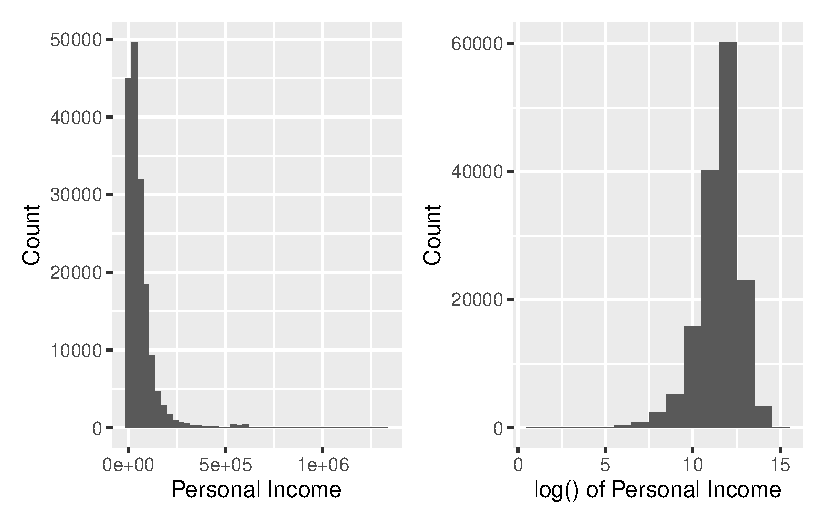
\includegraphics[keepaspectratio]{Group4_Final_Report_Project1_files/figure-pdf/eda-histograms-1.pdf}}

\begin{figure}[H]

{\centering \pandocbounded{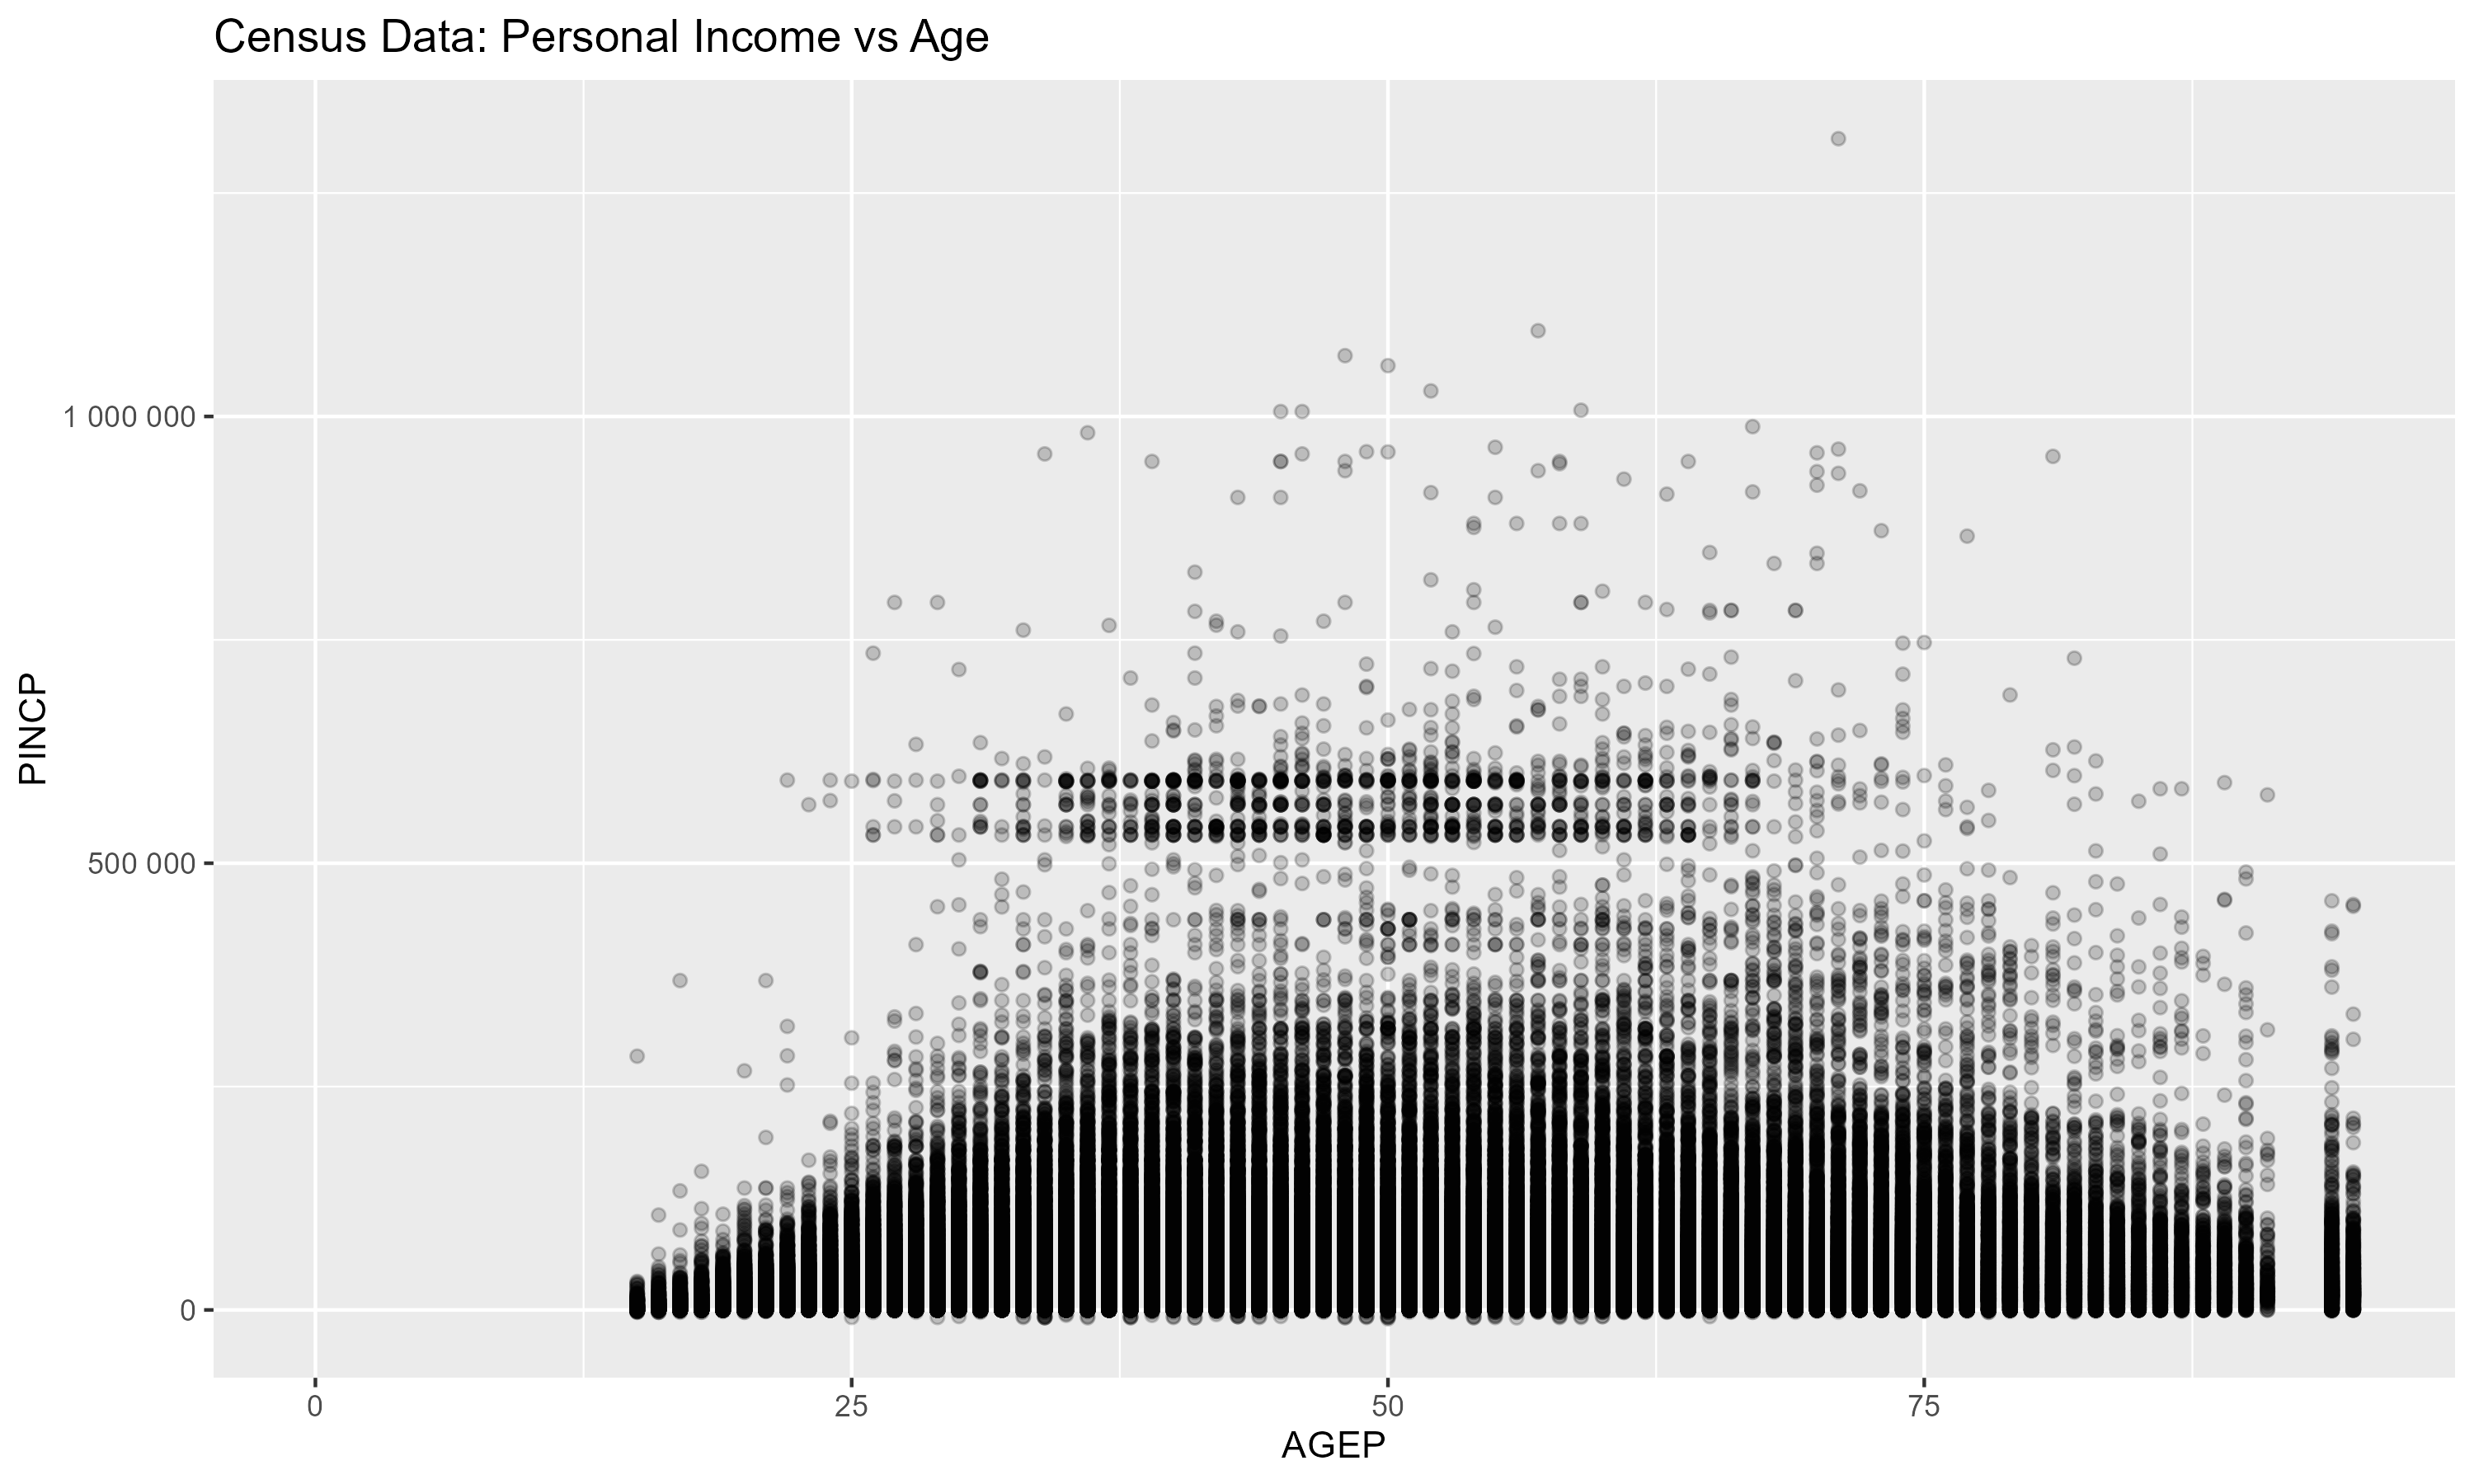
\includegraphics[keepaspectratio]{./eda-incomevage-plot.png}}

}

\caption{Distribution of personal income (PINCP) and log-transformed
income, along with income versus age.}

\end{figure}%

The above summary statistics indicate that income (PINCP) is highly
right-skewed, with a small number of individuals earning substantially
more than the median. Because of this skewness, we applied a log
transformation to the income response when evaluating linear model fit
for the final report. The scatterplot of income versus age suggests a
nonlinear relationship: income tends to increase with age early in life,
plateau in middle age, and decline slightly at older ages. This pattern
suggests the inclusion of a quadratic age term in the regression model.

\begin{figure}[H]

{\centering \pandocbounded{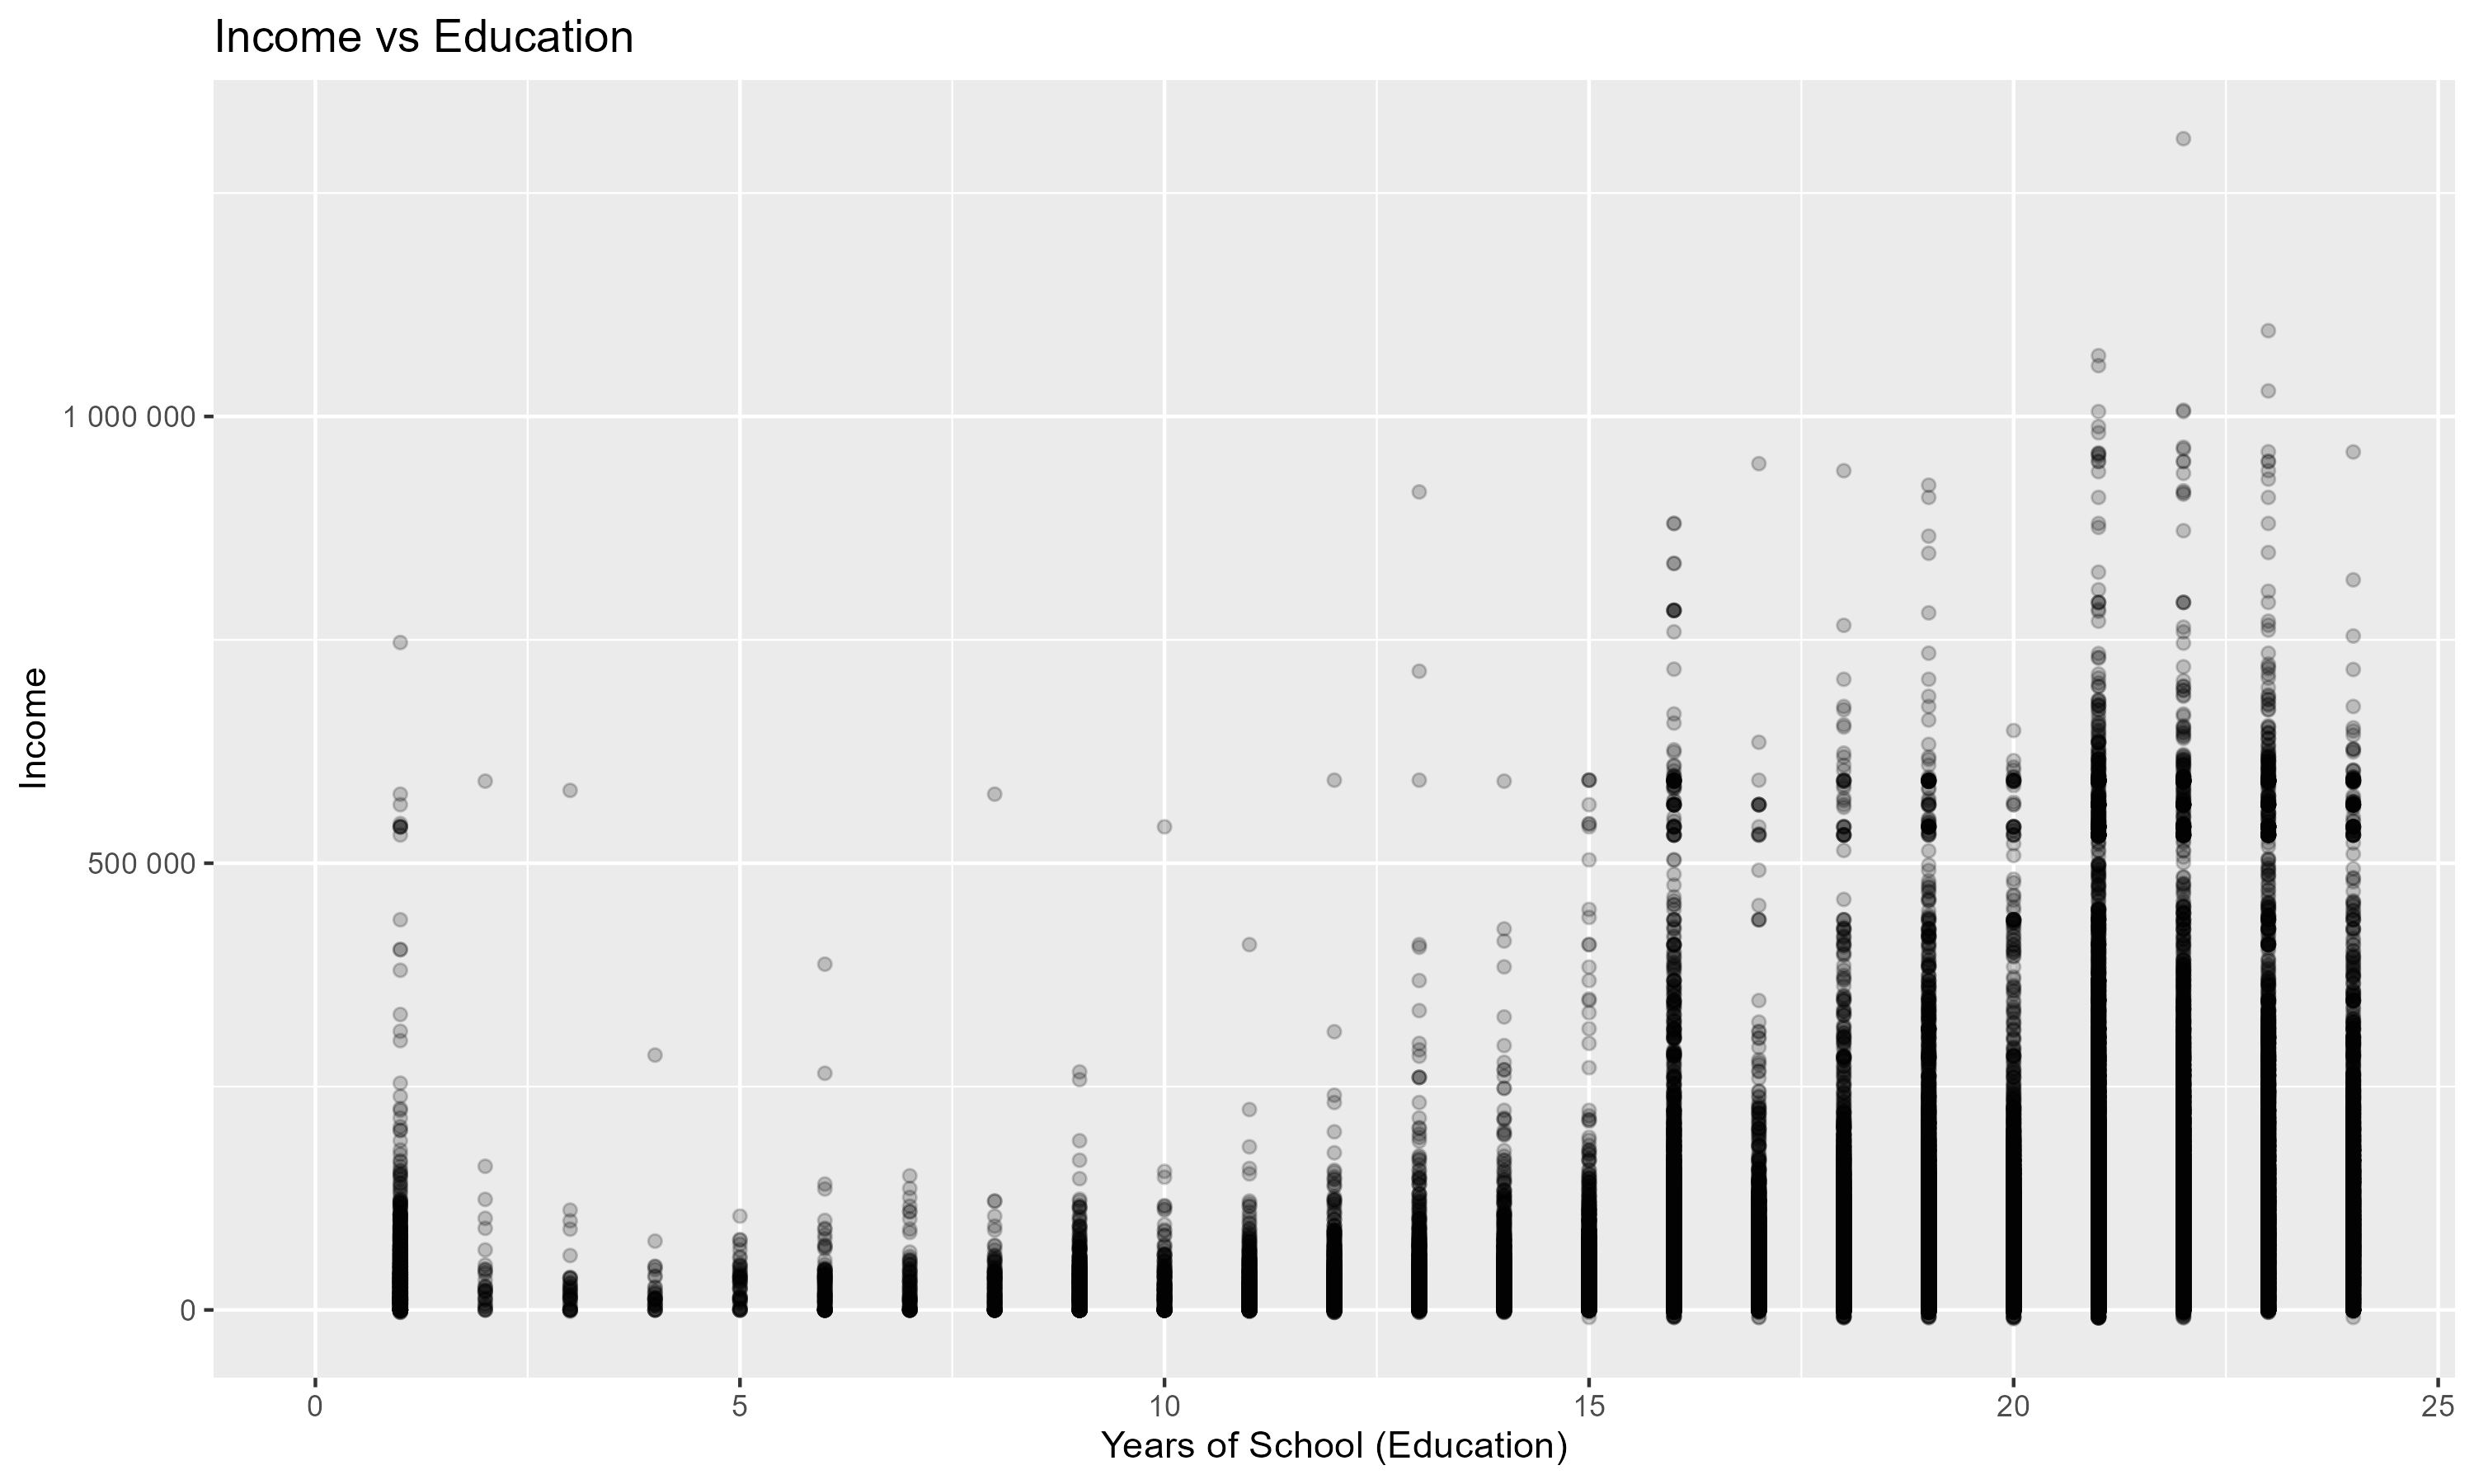
\includegraphics[keepaspectratio]{./eda-incomeved-plot.png}}

}

\caption{elationship between income and years of education.}

\end{figure}%

\pandocbounded{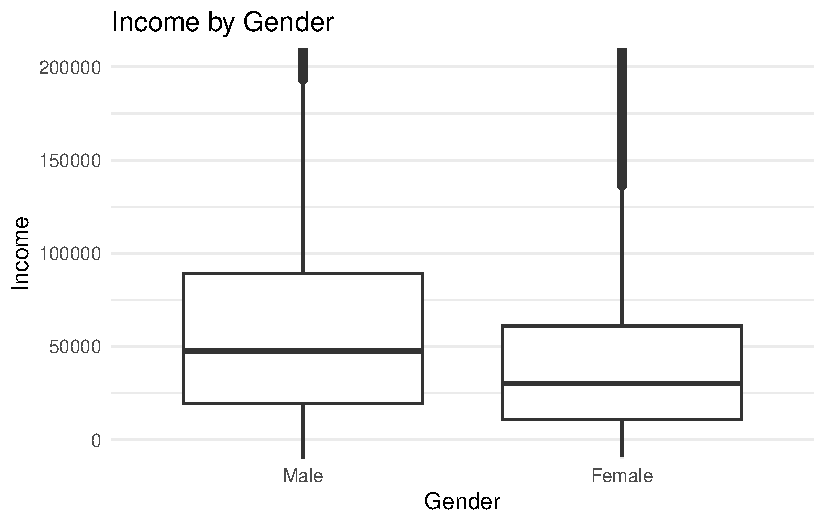
\includegraphics[keepaspectratio]{Group4_Final_Report_Project1_files/figure-pdf/eda-incomevgender-1.pdf}}

\pandocbounded{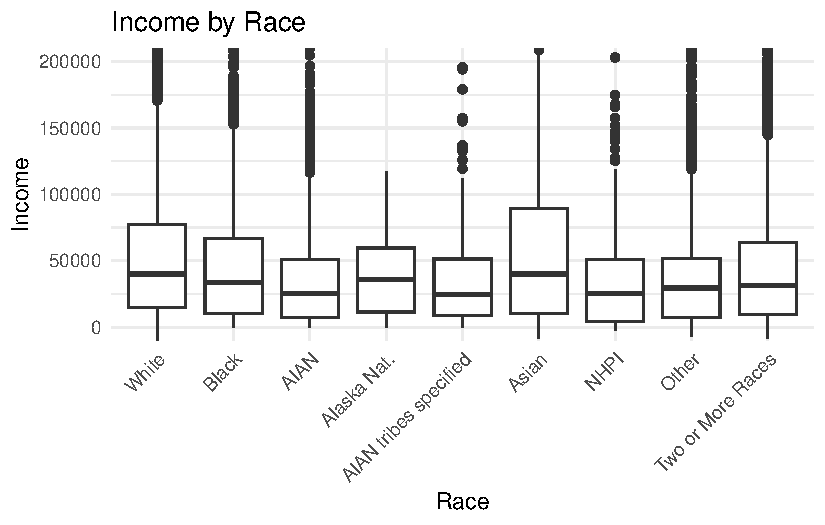
\includegraphics[keepaspectratio]{Group4_Final_Report_Project1_files/figure-pdf/eda-incomevrace-1.pdf}}

attainment corresponding to higher earnings. Boxplots of income by
gender and race reveal differences in median income across groups,
supporting their inclusion as categorical predictors. Overall, the
exploratory analysis suggests that income is influenced by multiple
demographic and socioeconomic factors, and that nonlinear effects,
particularly for age, should be incorporated into the model.

\subsection{Exploratory Data Analysis: Question
2}\label{exploratory-data-analysis-question-2}

We use the full Oregon sample from pums\_clean (all ages and labor force
statuses) to capture coverage gaps among non-citizens, including those
outside the workforce. After dropping missing values for insurance
(HICOV), income (POVPIP), and citizenship (CIT), the final sample
includes 197,991 residents.

The outcome is being uninsured (1 = uninsured, 0 = insured). Income is
measured with POVPIP (percent of the poverty line), aligning with
Medicaid and ACA thresholds. Education (SCHL) is grouped into six
levels, and employment (ESR\_group) into five categories to separate
labor force from citizenship effects. Household size (NP), full
citizenship categories (CIT), and controls for age, race, and Hispanic
origin are also included.

The exploratory analysis reveals a stark and consistent coverage gap by
citizenship status. Non-citizens in Oregon are uninsured at roughly 26\%
--- about 21 percentage points higher than US-born residents, whose rate
sits between 4--9\% across all citizen categories (Figure 1). Income
matters: uninsured residents are concentrated below 200\% of the poverty
line, and POVPIP clearly tracks coverage status (Figure 2). But income
tells only part of the story --- uninsured individuals appear at every
income level, particularly in the 200--400\% range, suggesting other
forces are at work. Figure 3 makes this plain. Even among the employed,
where employer-sponsored coverage is most accessible, non-citizens are
uninsured at \textasciitilde27\% compared to \textasciitilde6\% for
US-born workers --- a gap of over 20 percentage points within the same
employment category. Unemployed non-citizens face compounding
disadvantage at \textasciitilde42\%, excluded simultaneously from
employer coverage and from many public programs available to citizens in
identical economic circumstances. The pattern holds across income
levels, employment groups, and labor force status: citizenship status
appears to independently shape access to health insurance in Oregon,
over and above socioeconomic position. The regression models that follow
test whether this gap persists after controlling for income, education,
employment, household size, age, race, and Hispanic origin.

\pandocbounded{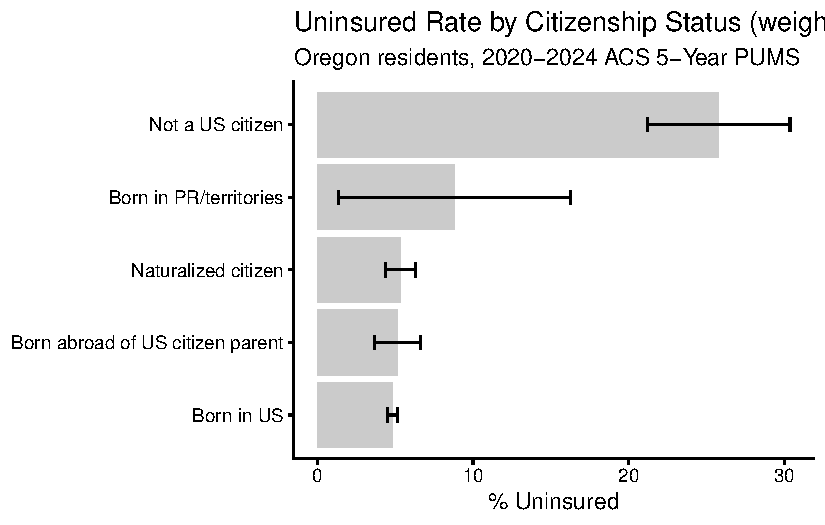
\includegraphics[keepaspectratio]{Group4_Final_Report_Project1_files/figure-pdf/q2-eda-citizenship-1.pdf}}

\begin{figure}[H]

{\centering \pandocbounded{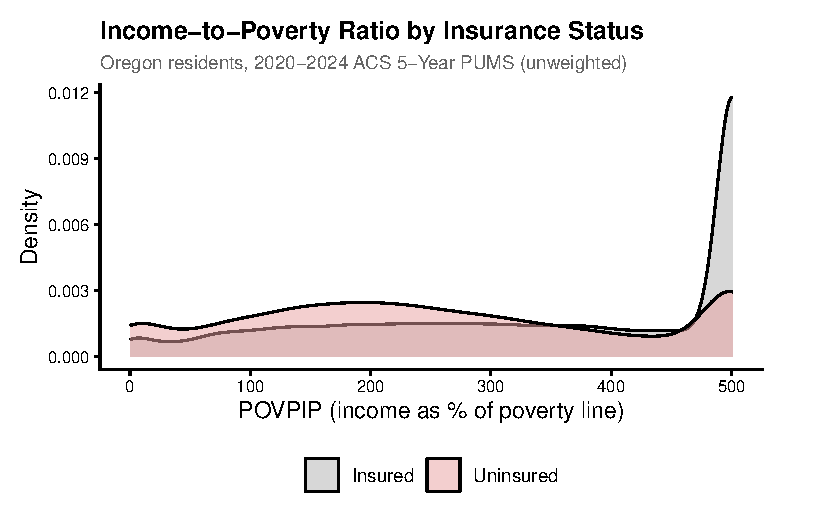
\includegraphics[keepaspectratio]{Group4_Final_Report_Project1_files/figure-pdf/q2-fig-povpip-1.pdf}}

}

\caption{Distribution of income-to-poverty ratio by insurance status.
Oregon residents, 2020-2024 ACS 5-Year PUMS (unweighted).}

\end{figure}%

\begin{figure}[H]

{\centering \pandocbounded{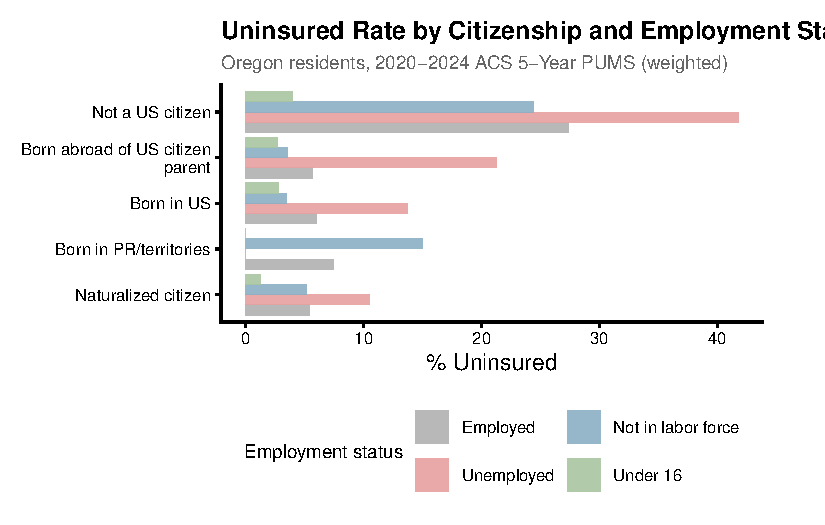
\includegraphics[keepaspectratio]{Group4_Final_Report_Project1_files/figure-pdf/q2-fig-cit-employment-1.pdf}}

}

\caption{Uninsured rate by citizenship status and employment group.
Oregon residents, 2020-2024 ACS 5-Year PUMS (weighted). Armed Forces
excluded due to small cell sizes.}

\end{figure}%

\subsubsection{Q1: Model Selection}\label{q1-model-selection}

Based on our analysis of the data, we fit multiple linear regression
models to assess how well income can be predicted from the selected
variables. The initial full model is:

\[Income = Age+Age^2+Education+Gender+Race+Birthplace+Household members\]

We also included models of the log income as well. Income is modeled as
a continuous response, and predictors include both continuous variables
(age, education, household members) and categorical variables (gender,
race, birthplace). A quadratic term for age is included to capture the
nonlinear relationship observed in the exploratory analysis.

A reduced model excluding birthplace and household members is also
considered due to weak initial evidence of its importance:

\[Income=Age+Age^2+Education+Gender+Race\]

\subsubsection{Q1: Model Checking and
Selection}\label{q1-model-checking-and-selection}

\begin{figure}[H]

{\centering \pandocbounded{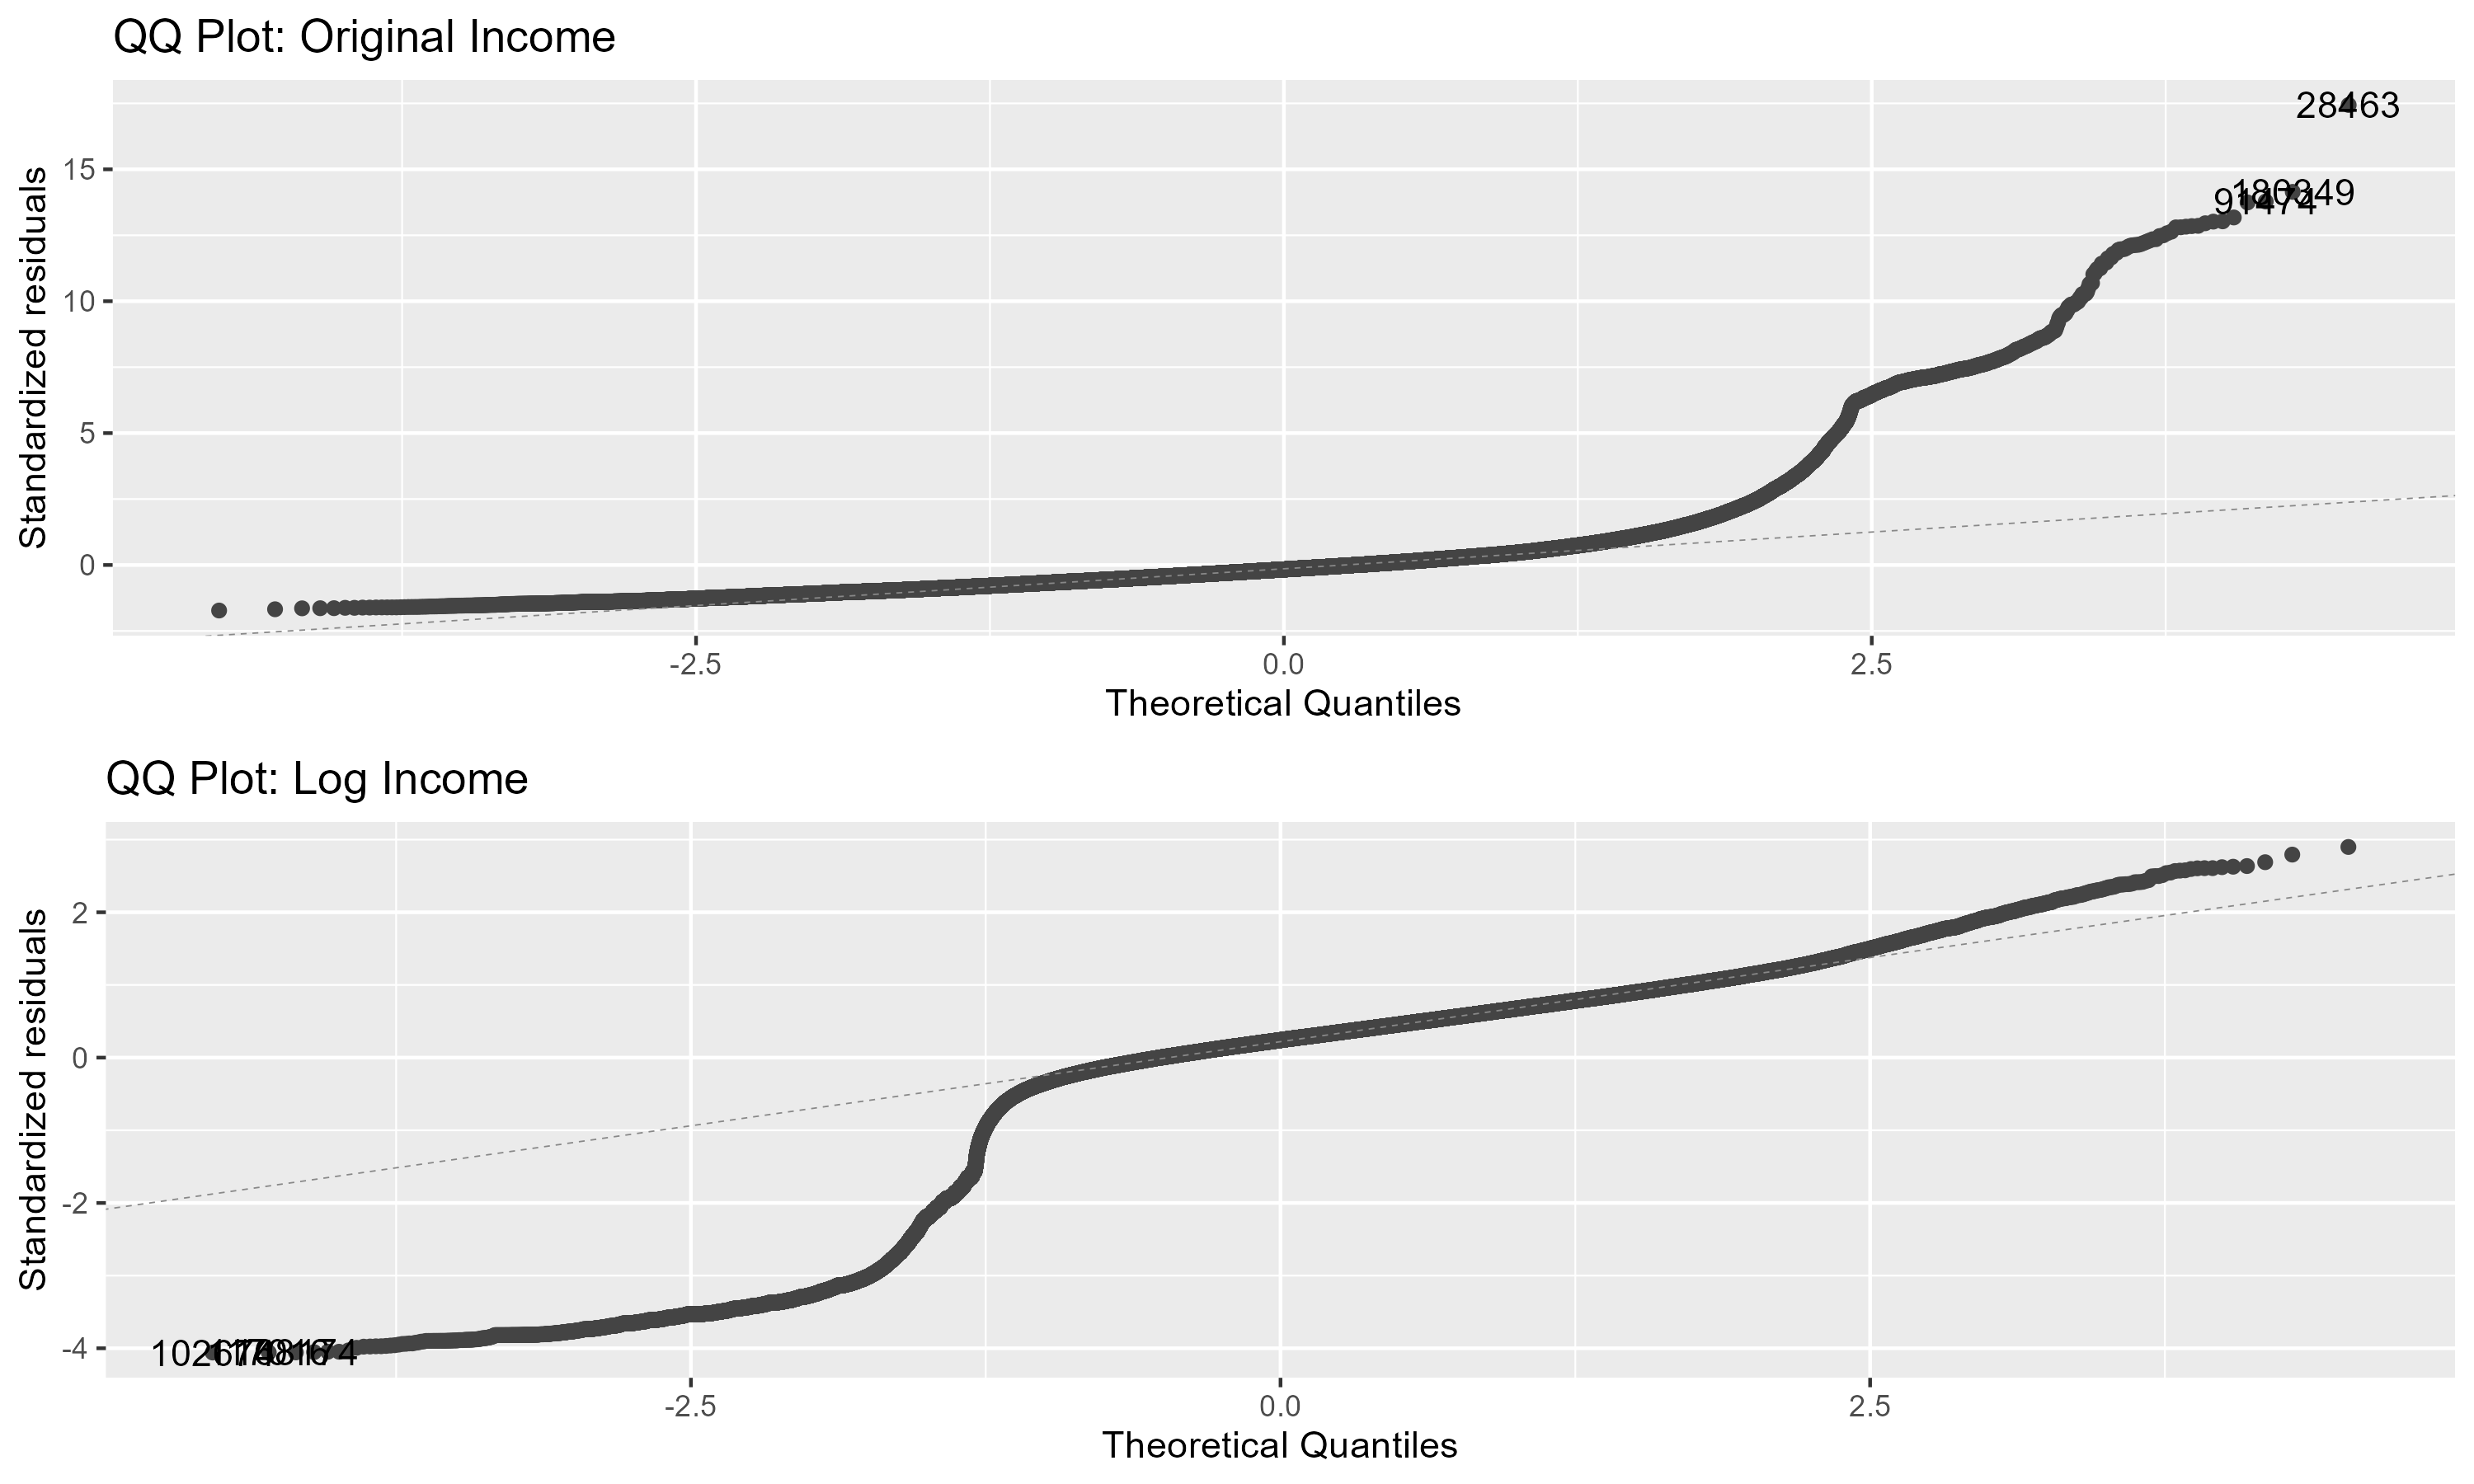
\includegraphics[keepaspectratio]{./q1-model-plots2.png}}

}

\caption{QQ plots of residuals from linear models using original and
log-transformed income.}

\end{figure}%

Model diagnostics were conducted to assess the validity of the linear
regression assumptions. Residual plots indicated non-constant variance
and right-skewness, which is consistent with the skewed distribution of
income. We also conducted and plotted a log transformation of income.
The residual plots suggest improves overall fit, although the
untransformed model is retained for interpretability. Multicollinearity
was assessed using variance inflation factors (VIF). All predictors
showed low VIF values (near 1), except for age and age squared, which
exhibited moderate collinearity. This is expected due to the polynomial
relationship and does not invalidate the model. Centering age can reduce
this collinearity but does not change model fit.

Alongside the linear model approach, we also evaluated a larger model
using penalized linear regression. We separated Personal Income (PINCP)
and all other variables in the dataset, leaving out other income related
variables, then ran a series of lasso methods on the data to find a
model of best fit and of a reduced model (yet still expanded from our
linear approach) for better performance.

While the initial linear regression models were based on a limited set
of predictors identified through exploratory analysis, they may omit
relevant variables and fail to capture the full complexity of the data.
Given the large number of available predictors in the ACS dataset, we
expanded the modeling approach to consider a broader set of variables.
To manage the resulting increase in dimensionality and potential
multicollinearity, we employed penalized linear regression using the
LASSO method. LASSO allows us to identify a more targeted set of
predictors while maintaining predictive performance. The regularization
parameter was selected using cross-validation, with the
\(\lambda_{lse}\) model chosen to balance model simplicity and accuracy.
Figure @q1-lasso-cv-plot presents the cross-validation curve used to
select the optimal regularization parameter. While \(\lambda_{min}\)
achieves the lowest prediction error, the \(\lambda_{lse}\) model
provides comparable performance with substantially fewer predictors and
is therefore selected for interpretation. The resulting set of non-zero
coefficients identifies the most influential variables in predicting
income.

\begin{figure}[H]

{\centering \pandocbounded{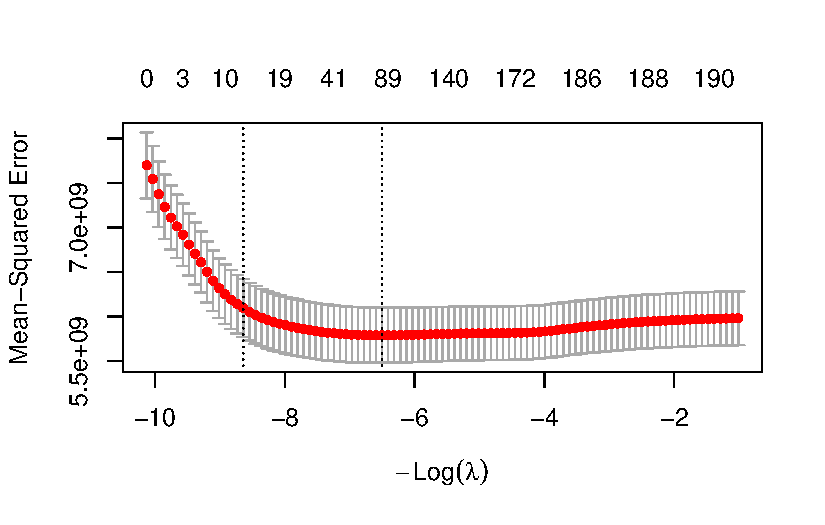
\includegraphics[keepaspectratio]{Group4_Final_Report_Project1_files/figure-pdf/q1-lasso-cv-plot-1.pdf}}

}

\caption{Cross-validation curve for the LASSO model showing mean squared
error across values of the regularization parameter lambda.}

\end{figure}%

\begin{table}
\fontsize{12.0pt}{14.0pt}\selectfont
\begin{tabular*}{\linewidth}{@{\extracolsep{\fill}}lr}
\toprule
Variable & Coefficient \\ 
\midrule\addlinespace[2.5pt]
AGEP & 133.39 \\ 
SEXFemale & -10,114.75 \\ 
MARNever married & -5,842.34 \\ 
RELSHIPP & -773.88 \\ 
SCHL & 2,776.24 \\ 
COWSelf-emp not incorporated & 3,803.42 \\ 
WKHP & 1,270.42 \\ 
WKWN & 520.95 \\ 
PUMA05114 & 26,557.74 \\ 
PUMA06721 & 755.32 \\ 
TENRented & -11,765.93 \\ 
HISP\_binaryNot Hispanic & 11,661.62 \\ 
\bottomrule
\end{tabular*}
\end{table}

\subsubsection{Q1: Inferences}\label{q1-inferences}

In the multiple linear regression model, several predictors show
statistically significant associations with income. Education has a
strong positive effect, indicating that higher educational attainment is
associated with increased income, holding other variables constant. Age
exhibits a nonlinear relationship with income, with the quadratic term
confirming that earnings increase early in life and level off or decline
at older ages. Gender and race also show statistically significant
differences, suggesting persistent disparities in income across
demographic groups. While the overall explanatory power of the model is
modest, these results indicate that key demographic and socioeconomic
factors contribute meaningfully to variation in income. The LASSO
results support these findings by selecting a similar subset of
variables, reinforcing the importance of education, labor supply, and
demographic characteristics as key predictors of income.

\subsection{Question2:}\label{question2}

After conducting exploratory data analysis of citizenship, employment
status, and their relationship to insurance coverage, we pose the
following question:

What is the magnitude of the health insurance coverage gap by
citizenship status among Oregon residents, and does this gap persist
after adjusting for income, education, employment status, household
size, age, race, and Hispanic origin?

\subsubsection{Data and Variables for Question
2}\label{data-and-variables-for-question-2}

Our data sample uses the full Oregon resident population in pums\_clean
(n = 197,991), including all ages and labor force statuses. This avoids
worker-only restriction, which would underrepresent non-citizens most at
risk of uninsurance. Observations missing key variables (HICOV, POVPIP,
or CIT) were excluded prior to analysis.

The response variable is lacking health insurance, coded as a binary
integer (1 = uninsured, 0 = insured) by inverting HICOV. It is stored as
an integer rather than a logical variable to ensure compatibility with
svyby() in the survey package.

Citizenship status (CIT) is the main predictor and is kept in all five
categories---U.S.-born, born in Puerto Rico/territories, born abroad to
U.S. citizen parents, naturalized citizen, and non-citizen---to capture
differences in legal eligibility for coverage.

Income is measured using the income-to-poverty ratio (POVPIP), which is
preferred over raw income because eligibility for Medicaid and ACA
subsidies is defined relative to the federal poverty line. Education
(SCHL) is collapsed into six attainment levels, and employment status
(ESR) into five categories to separate labor market effects from
citizenship effects.

Household size (NP), age (AGEP), race (RAC1P), and Hispanic origin
(HISP\_binary) are included as additional controls to adjust for
demographic differences across citizenship groups.

\subsubsection{Model Structure}\label{model-structure}

Two survey-weighted logistic regression models are estimated. The
reduced model includes only citizenship status and income-to-poverty
ratio, providing a baseline estimate of the raw citizenship coverage
gap. The full model adds education, employment status, household size,
age, race, and Hispanic origin to adjust for socioeconomic and
demographic differences. Comparing the two models shows how much of the
citizenship gap is explained by income, education, and other
characteristics, and how much remains due to structural and legal
barriers to coverage.

\subsubsection{Estimation Method}\label{estimation-method}

Both models are estimated using survey-weighted logistic regression
(svyglm) with a quasibinomial family and logit link. The quasibinomial
specification allows for overdispersion by estimating a dispersion
parameter rather than fixing it at one, producing more reliable standard
errors for survey data. The survey design clusters observations by PUMA
and applies person weights (PWGTP) to approximate the PUMS sampling
structure.

\subsubsection{Model Comparison and Fit}\label{model-comparison-and-fit}

Model fit is evaluated using quasi-AIC and McFadden's pseudo \(R^2\),
both compared to an intercept-only null model. The added contribution of
each set of predictors is tested using Wald F-tests (regTermTest()),
which is appropriate for survey-weighted models in place of likelihood
ratio tests. Multicollinearity is assessed using generalized variance
inflation factors (GVIF).

Ridge regression was considered but not used, since the large sample
size and relatively small number of predictors make regularization
unnecessary, and interpretability of odds ratios is central to the
research question on citizenship effects.

\subsubsection{Occupation}\label{occupation}

Occupation (OCCP) is excluded from the Q2 model even though it is
available in the dataset. It contains over 500 SOC codes, and collapsing
them into broad categories introduced ambiguity in classification. More
importantly, including occupation would restrict the analysis to
employed individuals, reintroducing a labor force bias that the
full-population design is intended to avoid. Employment status
(ESR\_group) is retained instead, as it captures labor market attachment
without excluding non-workers.

\begin{verbatim}

Call:
svyglm(formula = UNINSURED ~ CIT + POVPIP + SCHL_group + ESR_group + 
    NP + AGEP + RAC1P + HISP_binary, design = svy_q2, family = quasibinomial(link = "logit"))

Survey design:
svydesign(ids = ~PUMA, weights = ~PWGTP, data = pums_q2, nest = TRUE)

Coefficients:
                                                        Estimate Std. Error
(Intercept)                                           -0.5338148  0.0899134
CITBorn in PR/territories                              0.4763159  0.4719828
CITBorn abroad of US citizen parent                    0.1347098  0.1549335
CITNaturalized citizen                                 0.2718124  0.0786442
CITNot a US citizen                                    1.5349141  0.0916244
POVPIP                                                -0.0023268  0.0001624
SCHL_groupHigh school or GED                          -0.1003106  0.0479904
SCHL_groupSome college                                -0.4158448  0.0496661
SCHL_groupAssociate's degree                          -0.5608882  0.0663859
SCHL_groupBachelor's degree                           -0.9286850  0.0545245
SCHL_groupGraduate degree                             -1.5769650  0.1023404
ESR_groupUnemployed                                    0.4391694  0.0619491
ESR_groupNot in labor force                           -0.5805822  0.0448936
ESR_groupArmed Forces                                 -1.7437037  0.5688611
ESR_groupUnder 16                                     -2.0810375  0.0649215
NP                                                    -0.0230977  0.0136505
AGEP                                                  -0.0187777  0.0010633
RAC1PBlack or African American alone                  -0.5400432  0.1383882
RAC1PAmerican Indian alone                             0.3896566  0.1210496
RAC1PAlaska Native alone                               0.6544720  0.4978718
RAC1PAIAN tribes specified                             0.2105078  0.2341314
RAC1PAsian alone                                      -0.6652325  0.0863769
RAC1PNative Hawaiian and Other Pacific Islander alone -0.0691179  0.1913466
RAC1PSome other race alone                             0.1845607  0.0677438
RAC1PTwo or More Races                                -0.0042470  0.0662272
HISP_binaryNot Hispanic                               -0.1640314  0.0683813
                                                      t value Pr(>|t|)    
(Intercept)                                            -5.937 0.000219 ***
CITBorn in PR/territories                               1.009 0.339249    
CITBorn abroad of US citizen parent                     0.869 0.407181    
CITNaturalized citizen                                  3.456 0.007204 ** 
CITNot a US citizen                                    16.752 4.31e-08 ***
POVPIP                                                -14.329 1.68e-07 ***
SCHL_groupHigh school or GED                           -2.090 0.066159 .  
SCHL_groupSome college                                 -8.373 1.54e-05 ***
SCHL_groupAssociate's degree                           -8.449 1.43e-05 ***
SCHL_groupBachelor's degree                           -17.032 3.72e-08 ***
SCHL_groupGraduate degree                             -15.409 8.93e-08 ***
ESR_groupUnemployed                                     7.089 5.73e-05 ***
ESR_groupNot in labor force                           -12.932 4.06e-07 ***
ESR_groupArmed Forces                                  -3.065 0.013457 *  
ESR_groupUnder 16                                     -32.055 1.38e-10 ***
NP                                                     -1.692 0.124884    
AGEP                                                  -17.660 2.71e-08 ***
RAC1PBlack or African American alone                   -3.902 0.003606 ** 
RAC1PAmerican Indian alone                              3.219 0.010506 *  
RAC1PAlaska Native alone                                1.315 0.221176    
RAC1PAIAN tribes specified                              0.899 0.392019    
RAC1PAsian alone                                       -7.702 3.00e-05 ***
RAC1PNative Hawaiian and Other Pacific Islander alone  -0.361 0.726270    
RAC1PSome other race alone                              2.724 0.023439 *  
RAC1PTwo or More Races                                 -0.064 0.950271    
HISP_binaryNot Hispanic                                -2.399 0.039978 *  
---
Signif. codes:  0 '***' 0.001 '**' 0.01 '*' 0.05 '.' 0.1 ' ' 1

(Dispersion parameter for quasibinomial family taken to be 0.9694697)

Number of Fisher Scoring iterations: 6
\end{verbatim}

\begin{verbatim}
                                                    term    OR lower upper
1                                            (Intercept) 0.586 0.492 0.699
2                              CITBorn in PR/territories 1.610 0.638 4.061
3                    CITBorn abroad of US citizen parent 1.144 0.845 1.550
4                                 CITNaturalized citizen 1.312 1.125 1.531
5                                    CITNot a US citizen 4.641 3.878 5.554
6                                                 POVPIP 0.998 0.997 0.998
7                           SCHL_groupHigh school or GED 0.905 0.823 0.994
8                                 SCHL_groupSome college 0.660 0.599 0.727
9                           SCHL_groupAssociate's degree 0.571 0.501 0.650
10                           SCHL_groupBachelor's degree 0.395 0.355 0.440
11                             SCHL_groupGraduate degree 0.207 0.169 0.252
12                                   ESR_groupUnemployed 1.551 1.374 1.752
13                           ESR_groupNot in labor force 0.560 0.512 0.611
14                                 ESR_groupArmed Forces 0.175 0.057 0.533
15                                     ESR_groupUnder 16 0.125 0.110 0.142
16                                                    NP 0.977 0.951 1.004
17                                                  AGEP 0.981 0.979 0.983
18                  RAC1PBlack or African American alone 0.583 0.444 0.764
19                            RAC1PAmerican Indian alone 1.476 1.165 1.872
20                              RAC1PAlaska Native alone 1.924 0.725 5.105
21                            RAC1PAIAN tribes specified 1.234 0.780 1.953
22                                      RAC1PAsian alone 0.514 0.434 0.609
23 RAC1PNative Hawaiian and Other Pacific Islander alone 0.933 0.641 1.358
24                            RAC1PSome other race alone 1.203 1.053 1.373
25                                RAC1PTwo or More Races 0.996 0.875 1.134
26                               HISP_binaryNot Hispanic 0.849 0.742 0.970
\end{verbatim}

\begin{verbatim}
                   GVIF Df GVIF^(1/(2*Df))
CIT           89.865613  4        1.754685
POVPIP         2.854561  1        1.689545
SCHL_group   127.384791  5        1.623722
ESR_group    112.463573  4        1.804581
NP             3.250332  1        1.802868
AGEP           6.585002  1        2.566126
RAC1P       1728.527534  8        1.593510
HISP_binary    5.614661  1        2.369528
\end{verbatim}

\begin{verbatim}

Call:
svyglm(formula = UNINSURED ~ CIT + POVPIP, design = svy_q2, family = quasibinomial(link = "logit"))

Survey design:
svydesign(ids = ~PUMA, weights = ~PWGTP, data = pums_q2, nest = TRUE)

Coefficients:
                                      Estimate Std. Error t value Pr(>|t|)    
(Intercept)                         -2.1620131  0.0403675 -53.558  < 2e-16 ***
CITBorn in PR/territories            0.6508886  0.4755883   1.369   0.1816    
CITBorn abroad of US citizen parent  0.1166964  0.1576972   0.740   0.4652    
CITNaturalized citizen               0.1503903  0.0803683   1.871   0.0714 .  
CITNot a US citizen                  1.8206954  0.1083977  16.796  < 2e-16 ***
POVPIP                              -0.0027823  0.0001959 -14.201 1.37e-14 ***
---
Signif. codes:  0 '***' 0.001 '**' 0.01 '*' 0.05 '.' 0.1 ' ' 1

(Dispersion parameter for quasibinomial family taken to be 0.9964415)

Number of Fisher Scoring iterations: 6
\end{verbatim}

\begin{verbatim}
                                 term    OR lower upper
1                         (Intercept) 0.115 0.106 0.125
2           CITBorn in PR/territories 1.917 0.755 4.870
3 CITBorn abroad of US citizen parent 1.124 0.825 1.531
4              CITNaturalized citizen 1.162 0.993 1.361
5                 CITNot a US citizen 6.176 4.994 7.638
6                              POVPIP 0.997 0.997 0.998
\end{verbatim}

\pandocbounded{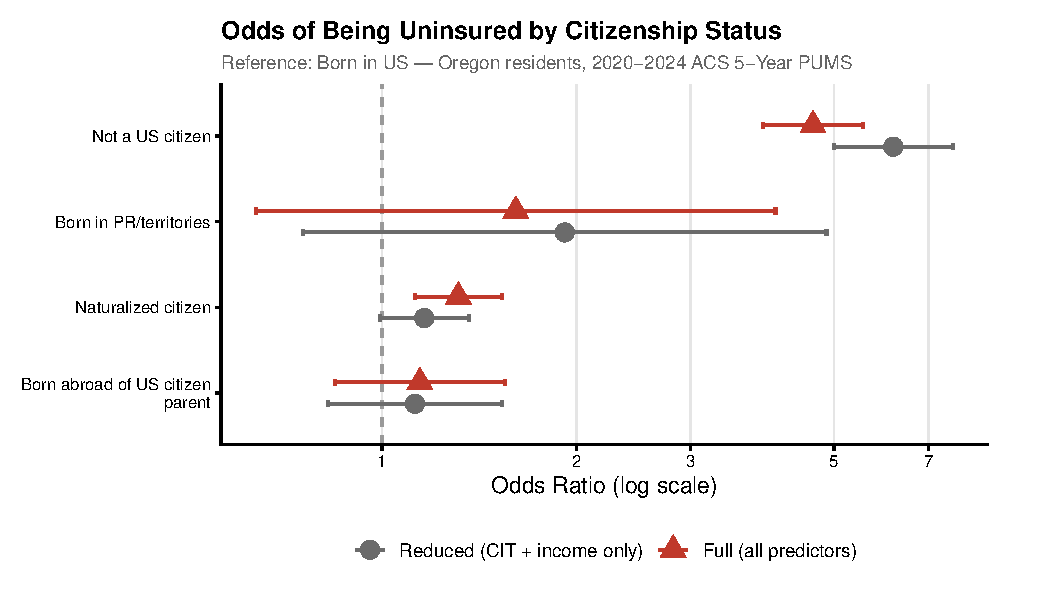
\includegraphics[keepaspectratio]{Group4_Final_Report_Project1_files/figure-pdf/q2-fig-forest-1.pdf}}

\begingroup\fontsize{10}{12}\selectfont

\begin{longtable}[t]{lcccc}
\caption{\label{tab:q2-results-table}Citizenship odds ratios, reduced vs full model (ref: Born in US). Change reflects OR shift after adding socioeconomic controls.}\\
\toprule
Citizenship Status & OR (Reduced) & OR (Full) & Change & p (Full)\\
\midrule
\textbf{\cellcolor{gray!10}{Not a US citizen}} & \textbf{\cellcolor{gray!10}{6.18}} & \textbf{\cellcolor{gray!10}{4.64}} & \textbf{\cellcolor{gray!10}{-24.9\%}} & \textbf{\cellcolor{gray!10}{< 0.001}}\\
Naturalized citizen & 1.16 & 1.31 & +12.9\% & 0.007\\
\cellcolor{gray!10}{Born in PR/territories} & \cellcolor{gray!10}{1.92} & \cellcolor{gray!10}{1.61} & \cellcolor{gray!10}{-16\%} & \cellcolor{gray!10}{0.339}\\
Born abroad of US citizen parent & 1.12 & 1.14 & +1.8\% & 0.407\\
\bottomrule
\end{longtable}
\endgroup{}

\begingroup\fontsize{10}{12}\selectfont

\begin{longtable}[t]{lcc}
\caption{\label{tab:q2-results-table}Model fit comparison: reduced vs full model.}\\
\toprule
Metric & Reduced Model & Full Model\\
\midrule
\cellcolor{gray!10}{McFadden R²} & \cellcolor{gray!10}{0.075} & \cellcolor{gray!10}{0.135}\\
Quasi-AIC & 81,935 & 76,687\\
\bottomrule
\end{longtable}
\endgroup{}

\subsubsection{Q2: Results}\label{q2-results}

The reduced model (citizenship + income) shows a large raw gap:
non-citizens have 6.18 times higher odds of being uninsured than
U.S.-born residents (95\% CI: 4.99--7.64, p \textless{} 0.001).
Naturalized citizens show a small, borderline elevation (OR = 1.16, p =
0.071).

In the full model, all major predictor blocks significantly improve
fit---education (F = 114.8), employment (F = 289.1), age (F = 311.9),
race (F = 14.1), and Hispanic origin (F = 5.75), all p \textless{}
0.05---except household size (F = 2.86, p = 0.125). Model fit increases
(pseudo R²: 0.075 → 0.135).

The citizenship gap remains large even after adjustment: non-citizens
still have 4.64 times higher odds of being uninsured (95\% CI:
3.88--5.55), and naturalized citizens also remain at higher risk (OR =
1.31, p = 0.007). This indicates that the gap is only partly explained
by socioeconomic factors.

Among controls, higher education is strongly protective (graduate degree
OR = 0.207), unemployment increases risk (OR = 1.55), and older age
reduces it (OR = 0.981 per year). Certain non-working groups have lower
odds due to public coverage programs. Some race effects persist, but
should be interpreted cautiously given overlap with citizenship and
ethnicity.

\subsubsection{Q2: Discussion}\label{q2-discussion}

There is a large and persistent citizenship gap in health insurance
coverage in Oregon. In the full survey-weighted logistic model,
non-citizens have 4.64 times higher odds of being uninsured than
U.S.-born residents (OR = 4.64, 95\% CI: 3.88--5.55, p \textless{}
0.001) after adjusting for income, education, employment, household
size, age, race, and Hispanic origin. This represents about a 25\%
reduction from the reduced model (OR = 6.18), meaning most of the gap is
not explained by observable socioeconomic differences. Naturalized
citizens also remain at elevated risk (OR = 1.31, p = 0.007), indicating
persistent disadvantage even after legal status changes.

Beyond citizenship, the strongest predictors of being uninsured are:

Education shows a strong gradient in coverage: individuals with a
graduate degree have substantially lower odds of being uninsured
compared to those without a high school diploma (OR = 0.207). Employment
status is also important, with unemployed individuals having higher odds
of being uninsured (OR = 1.55), although some non-working groups exhibit
lower uninsured rates due to eligibility for public programs such as
Medicare, Medicaid/CHIP, and military coverage. Age has a modest
protective effect, with the likelihood of being uninsured decreasing
slightly as age increases (OR \textasciitilde{} 0.981 per year). Race
and ethnicity effects are smaller and less stable after adjustment;
American Indians remain at elevated risk (OR = 1.48), while Asian
residents show lower odds of being uninsured, though these estimates
should be interpreted cautiously given multicollinearity among race,
ethnicity, and citizenship variables.

The citizenship gap in health insurance coverage is large and remains
robust even after controlling for socioeconomic and demographic factors,
indicating that it is driven more by structural and legal eligibility
constraints than by differences in population composition. Socioeconomic
characteristics explain only a small portion of the disparity, with most
of the gap persisting after adjustment. Additionally, naturalization
does not fully eliminate the elevated risk of being uninsured,
suggesting that residual barriers or disadvantages associated with
immigrant status continue even after obtaining citizenship.

Policy implications point to eligibility structure---not income or
employment---as the primary driver of coverage inequality. Expanding
coverage eligibility regardless of immigration status, reducing waiting
periods for immigrants, and improving enrollment access for non-citizens
are likely more impactful than labor-market or income-based
interventions alone.

\subsection{Question3: Can income be predicted from commute time,
location, and travel
ability?}\label{question3-can-income-be-predicted-from-commute-time-location-and-travel-ability}

Our third question for analysis was whether income can be predicted from
commute time, location, and travel ability. To do this, we design a
model to predict income and test it for prediction accuracy.

\subsubsection{Q3: Exploratory Analysis}\label{q3-exploratory-analysis}

First, we need to explore the dataset to see how variables are related
to income.

\begin{figure}[H]

{\centering \pandocbounded{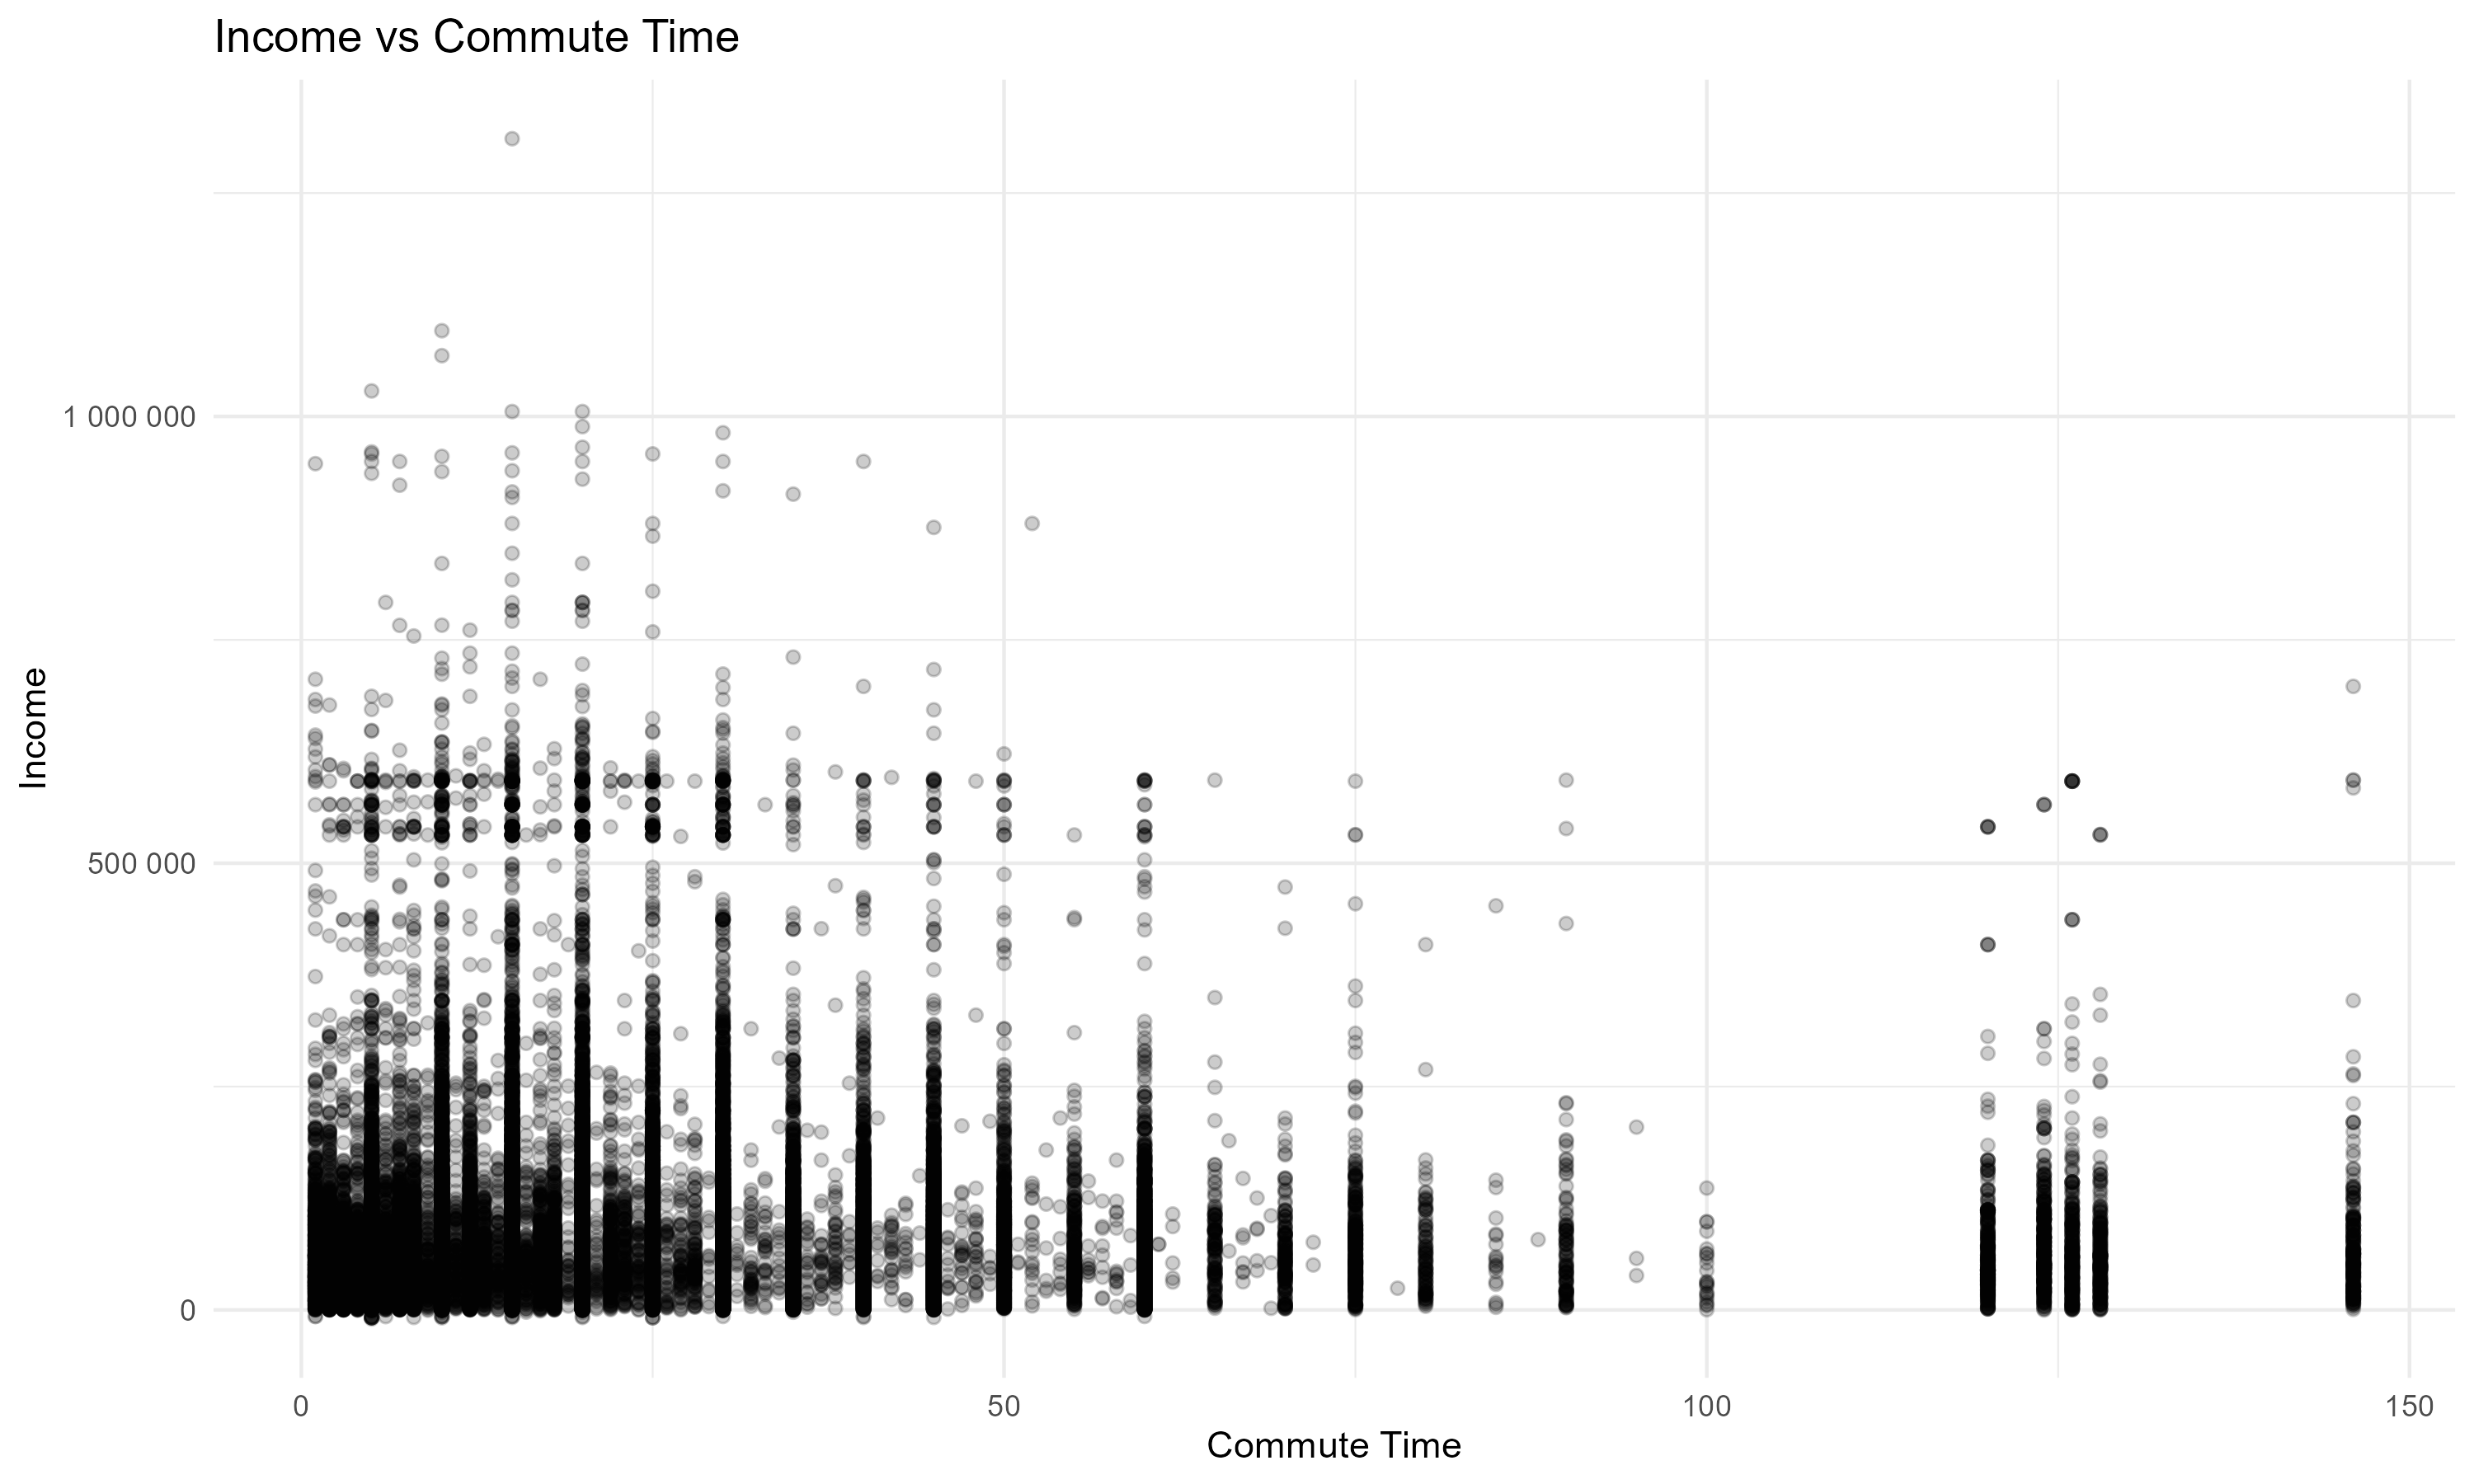
\includegraphics[keepaspectratio]{./q3-incomevcommutetime-plot.png}}

}

\caption{Relationship of personal income (PINCP) versus commute time
(JWMNP)}

\end{figure}%

In the above graph comparing commute time (JWMNP) and income (PINCP) we
see a sort of conflicting trend in the data. The maximum salary appears
to decrease as commutes increase, but there is also a significant
cluster of people with shorter commutes that make less money.

\begin{figure}[H]

{\centering \pandocbounded{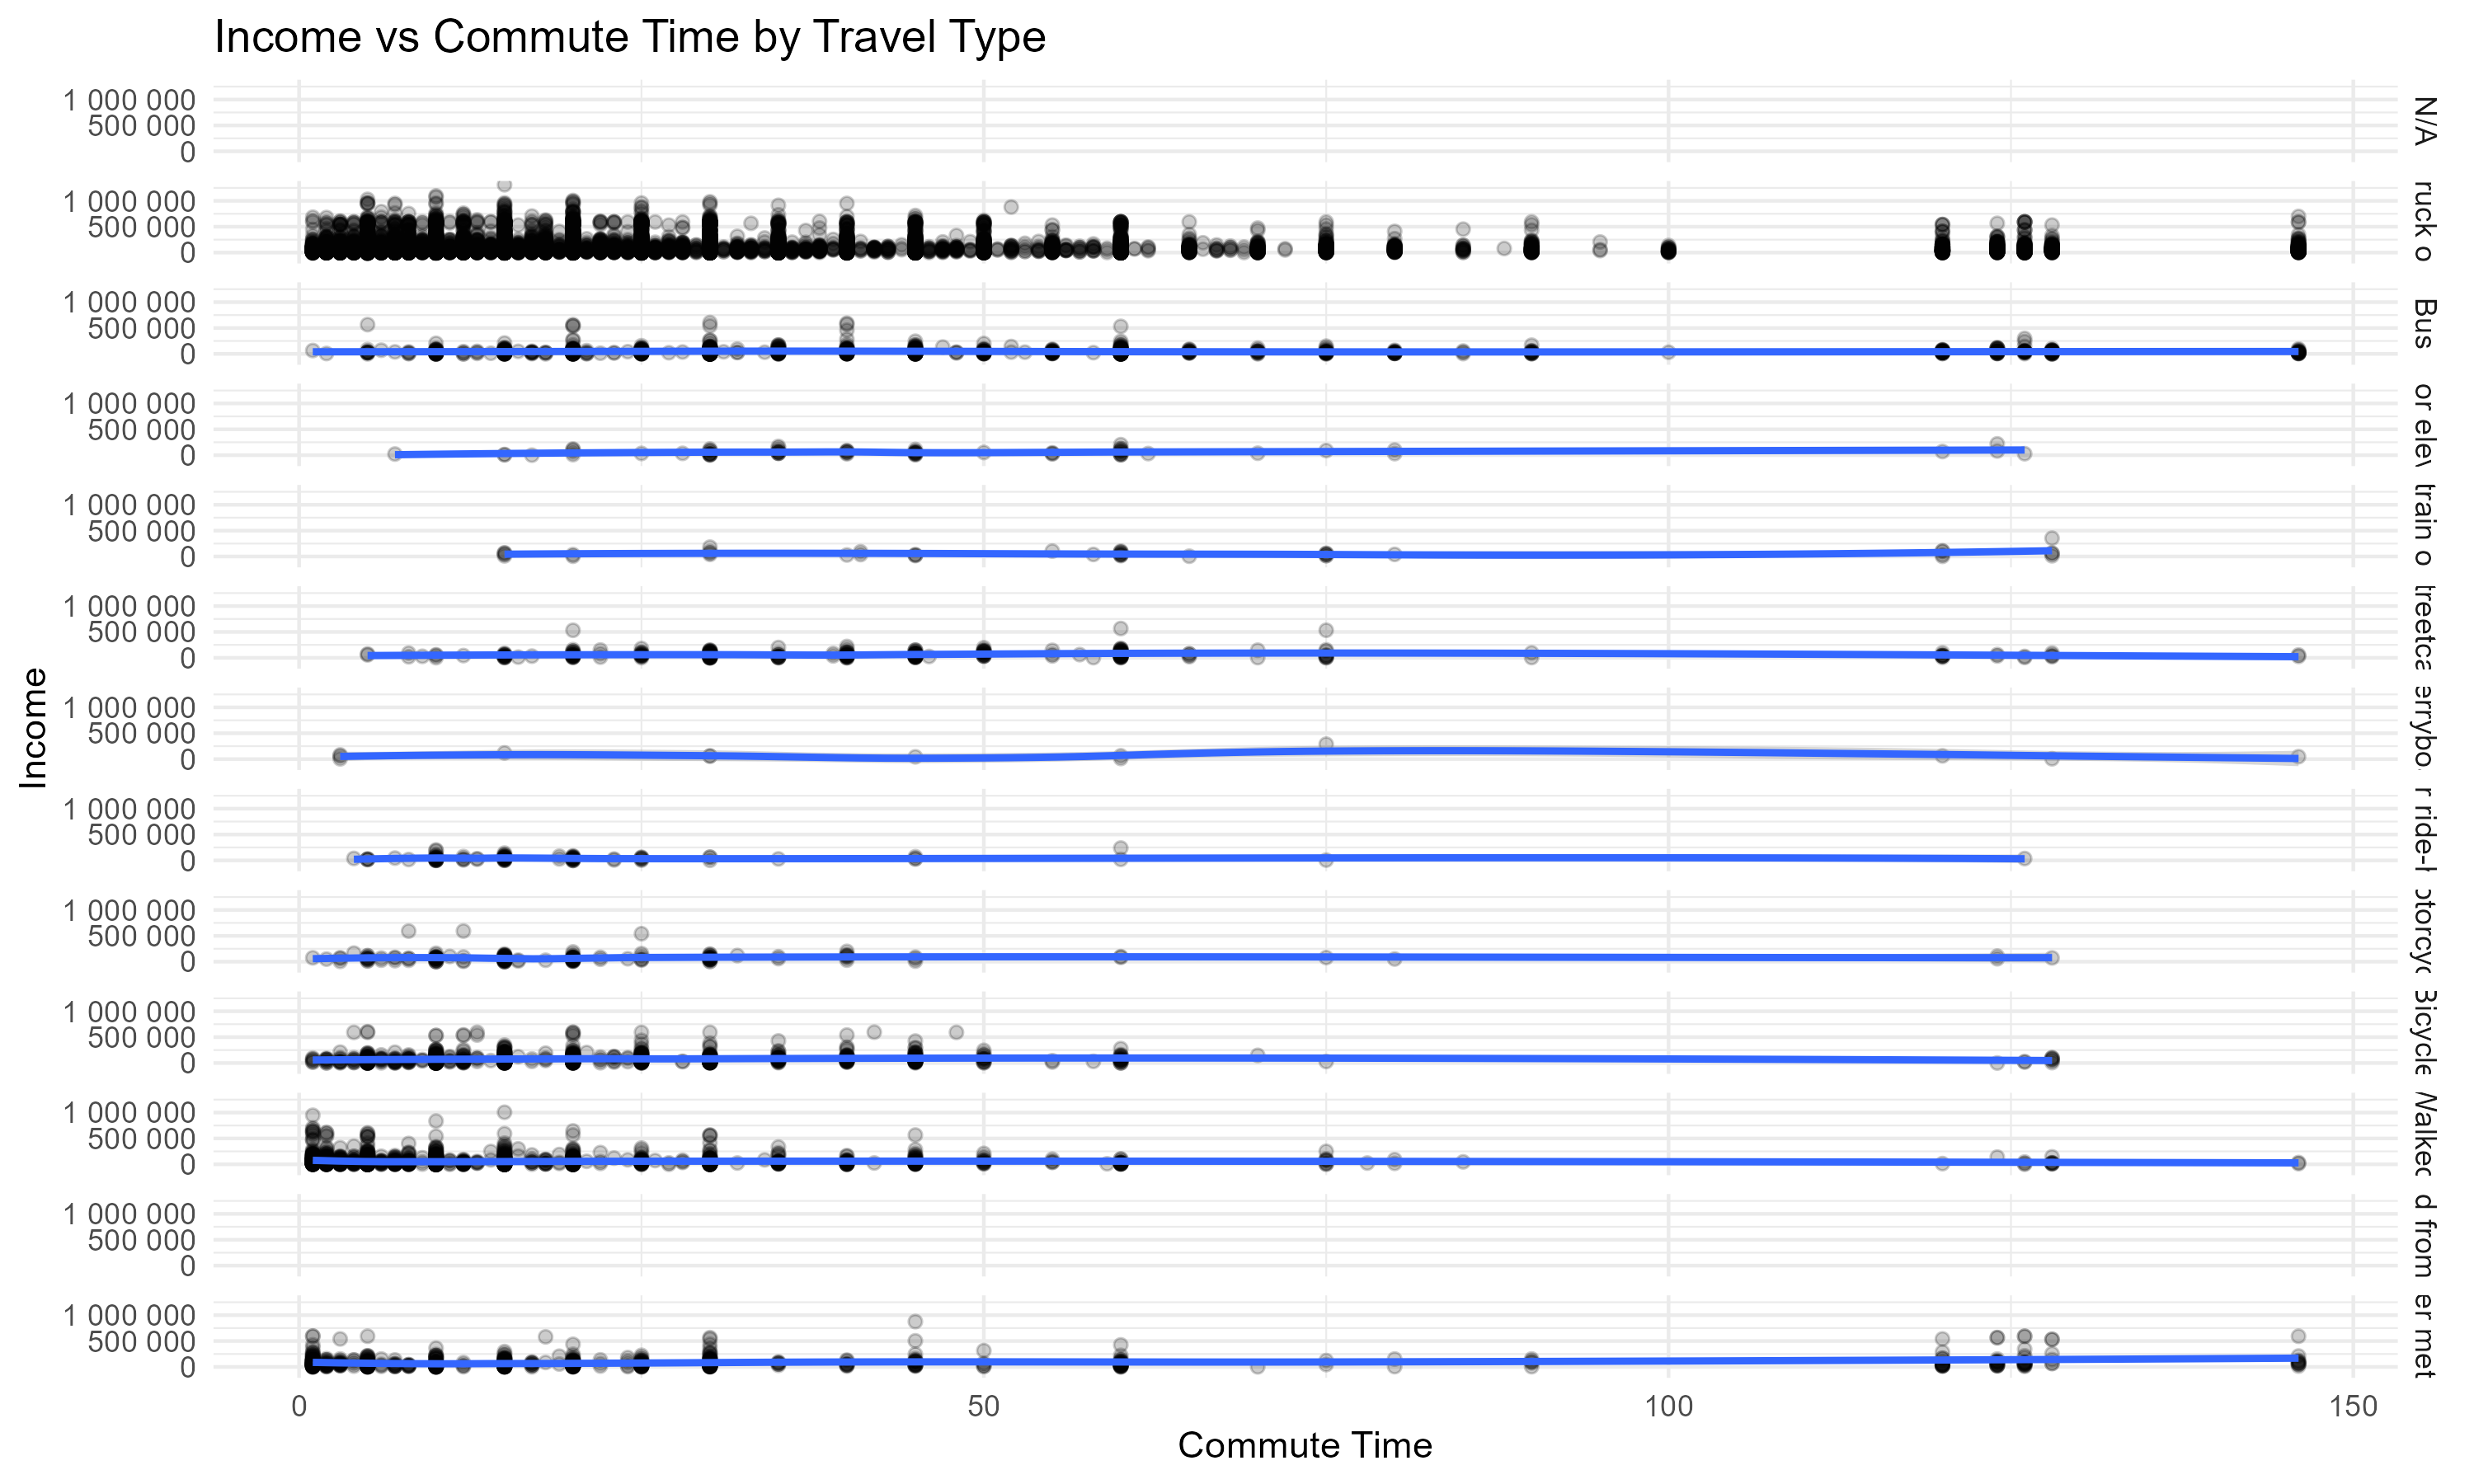
\includegraphics[keepaspectratio]{./q3-incomevcommutetimebytravel-plot.png}}

}

\caption{Relationship of personal income (PINCP) versus commute time
(JWMNP), faceted by type of travel (JWTRNS)}

\end{figure}%

The above graphs compare commute time and income but separated by mode
of transportation (JWTRNS). This breakdown shows in general, there
appears to be a slight decline as the length of commute by any method
increases and travel is overwhelmingly done by car.

\begin{figure}[H]

{\centering \pandocbounded{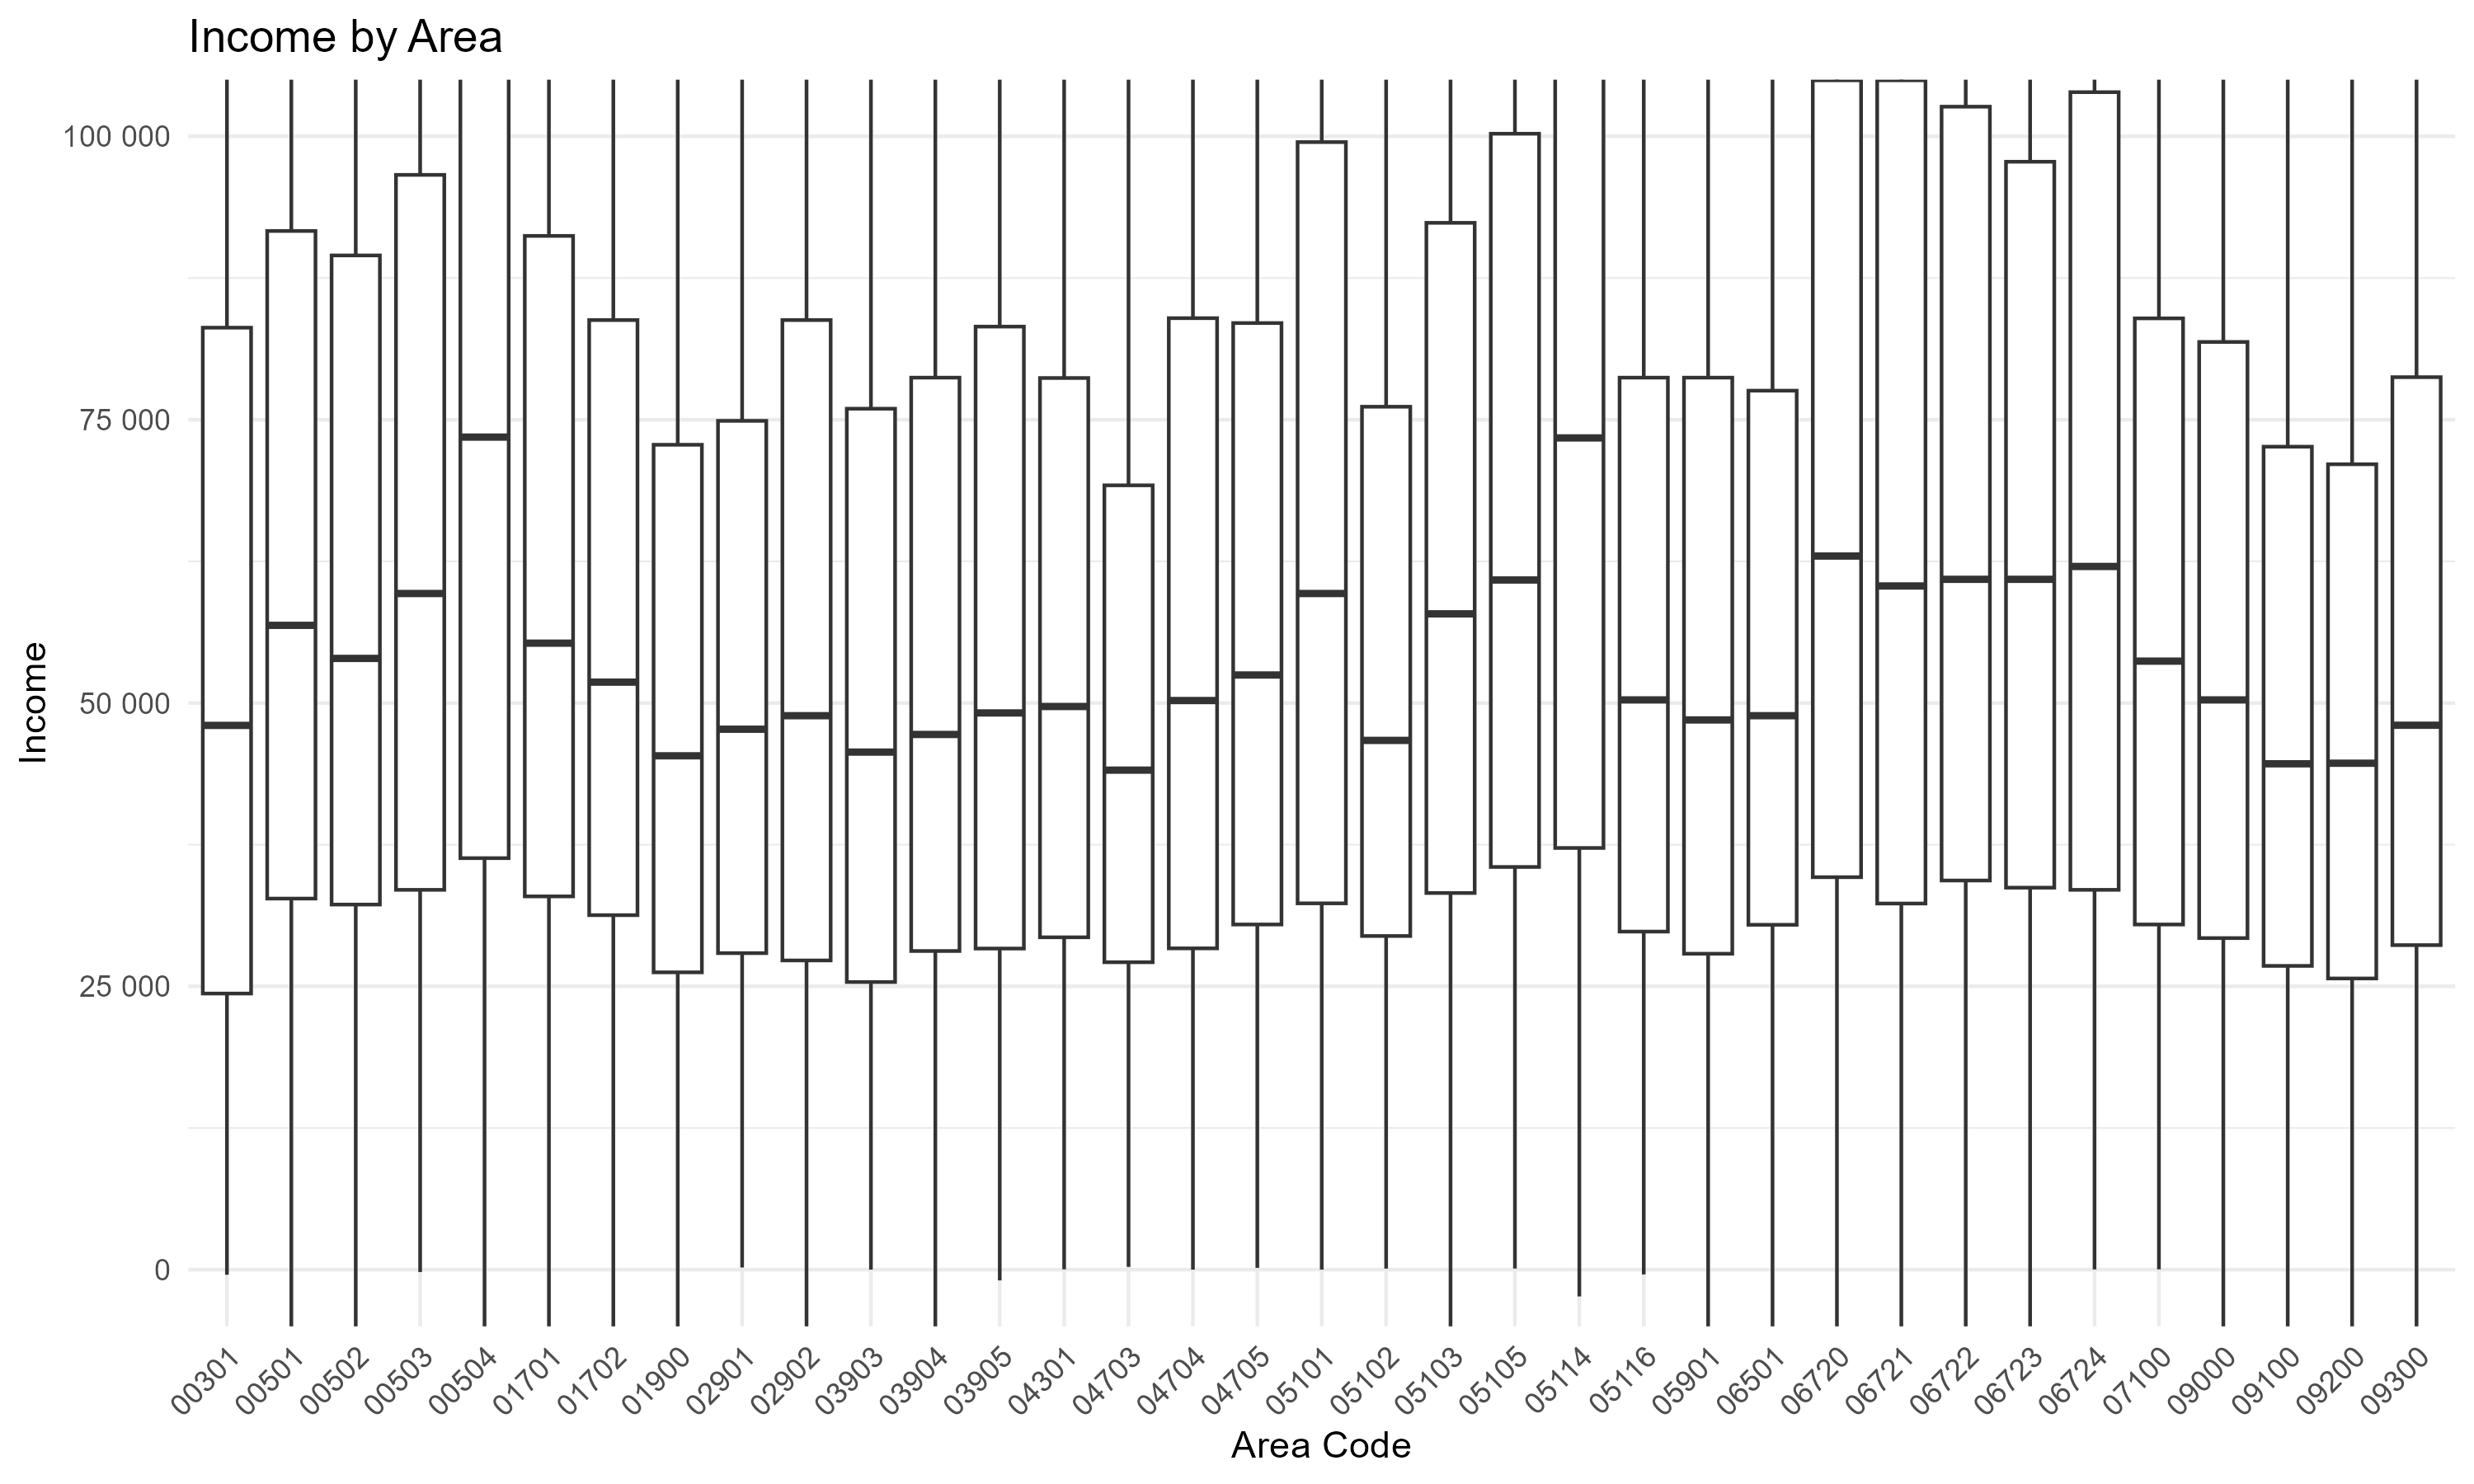
\includegraphics[keepaspectratio]{./q3-incomebyarea-plot.png}}

}

\caption{Distribution of personal income (PINCP) by Area Code (PUMA)}

\end{figure}%

Finally, we compare income based on geographic area. In the initial goal
of this question, we wanted the comparison to be city vs suburban vs
rural, but the dataset doesn't provide an effective way to determine
that categorization.

\subsubsection{Q3: Model Fitting}\label{q3-model-fitting}

Based on our exploratory analysis. The model we want to go with is:
PINCP \textasciitilde{} JWMNP + VEH + factor(JWTRNS) + factor(PUMA)

\subsubsection{Q3: Model Checking}\label{q3-model-checking}

\begin{verbatim}

Call:
lm(formula = PINCP ~ JWMNP + VEH + factor(JWTRNS) + factor(PUMA), 
    data = pums_clean)

Residuals:
    Min      1Q  Median      3Q     Max 
-137039  -40041  -16751   16118 1188385 

Coefficients:
                                                    Estimate Std. Error t value
(Intercept)                                         61780.36    1875.88  32.934
JWMNP                                                 144.22      14.78   9.759
VEH                                                   865.10     250.34   3.456
factor(JWTRNS)Bus                                  -36718.59    2241.16 -16.384
factor(JWTRNS)Subway or elevated rail              -30421.07    9563.39  -3.181
factor(JWTRNS)Long-distance train or commuter rail -28954.23   12403.52  -2.334
factor(JWTRNS)Light rail streetcar or trolley      -23088.80    4677.57  -4.936
factor(JWTRNS)Ferryboat                             -4081.81   21992.08  -0.186
factor(JWTRNS)Taxi or ride-hailing                 -33794.01    8142.71  -4.150
factor(JWTRNS)Motorcycle                             1954.96    6053.23   0.323
factor(JWTRNS)Bicycle                                 405.25    2315.22   0.175
factor(JWTRNS)Walked                               -16205.17    1537.66 -10.539
factor(JWTRNS)Other method                           4889.44    2758.39   1.773
factor(PUMA)00501                                    9823.20    2544.39   3.861
factor(PUMA)00502                                    1288.81    2577.87   0.500
factor(PUMA)00503                                    8563.27    2599.88   3.294
factor(PUMA)00504                                   53154.34    2538.33  20.941
factor(PUMA)01701                                   14187.74    2649.24   5.355
factor(PUMA)01702                                    1980.25    2421.07   0.818
factor(PUMA)01900                                   -8800.22    2569.80  -3.424
factor(PUMA)02901                                   -3206.00    2578.88  -1.243
factor(PUMA)02902                                    3142.28    2593.16   1.212
factor(PUMA)03903                                   -3066.71    2277.89  -1.346
factor(PUMA)03904                                   -1992.49    2455.99  -0.811
factor(PUMA)03905                                   -1739.17    2466.43  -0.705
factor(PUMA)04301                                   -5369.98    2415.31  -2.223
factor(PUMA)04703                                  -12980.43    2667.85  -4.866
factor(PUMA)04704                                    4410.69    2599.14   1.697
factor(PUMA)04705                                     630.09    2359.94   0.267
factor(PUMA)05101                                   12742.70    2407.72   5.292
factor(PUMA)05102                                   -4777.05    2478.53  -1.927
factor(PUMA)05103                                   11743.29    2467.93   4.758
factor(PUMA)05105                                   26858.44    2416.27  11.116
factor(PUMA)05114                                   56798.42    2309.05  24.598
factor(PUMA)05116                                   -4842.80    2330.47  -2.078
factor(PUMA)05901                                   -4093.25    2392.02  -1.711
factor(PUMA)06501                                   -4220.02    2362.37  -1.786
factor(PUMA)06720                                   16904.31    2384.63   7.089
factor(PUMA)06721                                   16581.16    2394.67   6.924
factor(PUMA)06722                                   12878.96    2407.62   5.349
factor(PUMA)06723                                   11581.02    2452.20   4.723
factor(PUMA)06724                                   24586.58    2538.17   9.687
factor(PUMA)07100                                    1366.56    2526.17   0.541
factor(PUMA)09000                                   -2655.04    2395.83  -1.108
factor(PUMA)09100                                   -6392.72    2346.44  -2.724
factor(PUMA)09200                                   -8526.70    2391.46  -3.565
factor(PUMA)09300                                   -1022.09    2377.76  -0.430
                                                   Pr(>|t|)    
(Intercept)                                         < 2e-16 ***
JWMNP                                               < 2e-16 ***
VEH                                                0.000549 ***
factor(JWTRNS)Bus                                   < 2e-16 ***
factor(JWTRNS)Subway or elevated rail              0.001468 ** 
factor(JWTRNS)Long-distance train or commuter rail 0.019580 *  
factor(JWTRNS)Light rail streetcar or trolley      7.99e-07 ***
factor(JWTRNS)Ferryboat                            0.852756    
factor(JWTRNS)Taxi or ride-hailing                 3.33e-05 ***
factor(JWTRNS)Motorcycle                           0.746725    
factor(JWTRNS)Bicycle                              0.861051    
factor(JWTRNS)Walked                                < 2e-16 ***
factor(JWTRNS)Other method                         0.076304 .  
factor(PUMA)00501                                  0.000113 ***
factor(PUMA)00502                                  0.617111    
factor(PUMA)00503                                  0.000989 ***
factor(PUMA)00504                                   < 2e-16 ***
factor(PUMA)01701                                  8.56e-08 ***
factor(PUMA)01702                                  0.413404    
factor(PUMA)01900                                  0.000616 ***
factor(PUMA)02901                                  0.213807    
factor(PUMA)02902                                  0.225609    
factor(PUMA)03903                                  0.178212    
factor(PUMA)03904                                  0.417207    
factor(PUMA)03905                                  0.480728    
factor(PUMA)04301                                  0.026198 *  
factor(PUMA)04703                                  1.14e-06 ***
factor(PUMA)04704                                  0.089704 .  
factor(PUMA)04705                                  0.789475    
factor(PUMA)05101                                  1.21e-07 ***
factor(PUMA)05102                                  0.053937 .  
factor(PUMA)05103                                  1.96e-06 ***
factor(PUMA)05105                                   < 2e-16 ***
factor(PUMA)05114                                   < 2e-16 ***
factor(PUMA)05116                                  0.037709 *  
factor(PUMA)05901                                  0.087047 .  
factor(PUMA)06501                                  0.074047 .  
factor(PUMA)06720                                  1.36e-12 ***
factor(PUMA)06721                                  4.42e-12 ***
factor(PUMA)06722                                  8.86e-08 ***
factor(PUMA)06723                                  2.33e-06 ***
factor(PUMA)06724                                   < 2e-16 ***
factor(PUMA)07100                                  0.588536    
factor(PUMA)09000                                  0.267782    
factor(PUMA)09100                                  0.006443 ** 
factor(PUMA)09200                                  0.000363 ***
factor(PUMA)09300                                  0.667302    
---
Signif. codes:  0 '***' 0.001 '**' 0.01 '*' 0.05 '.' 0.1 ' ' 1

Residual standard error: 79250 on 73505 degrees of freedom
  (124439 observations deleted due to missingness)
Multiple R-squared:  0.04133,   Adjusted R-squared:  0.04073 
F-statistic: 68.89 on 46 and 73505 DF,  p-value: < 2.2e-16
\end{verbatim}

According to the summary analysis of the model, every variable is
statistically significant at p: 0.05 level (or at least some values of
the categorical variables, even if not every value). Next we want to
check the residuals.

\pandocbounded{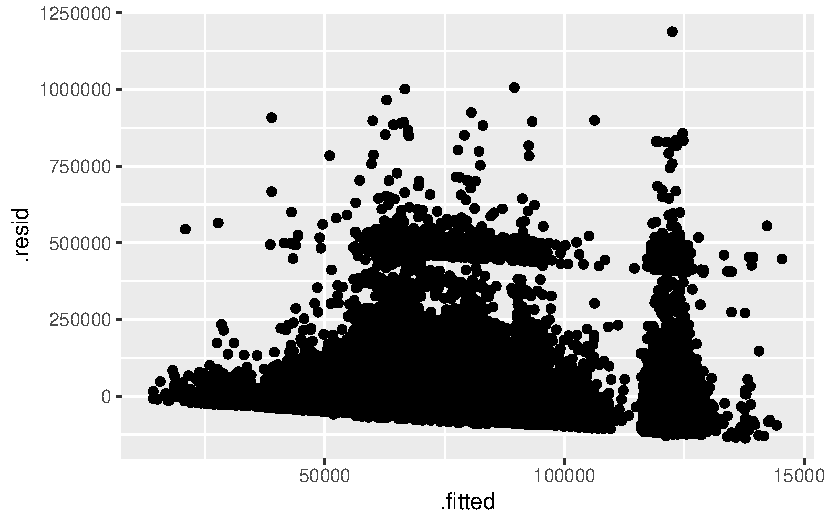
\includegraphics[keepaspectratio]{Group4_Final_Report_Project1_files/figure-pdf/q3-model-residuals-1.pdf}}

In graphing the residuals, we can see there is still a slight downward
trend in the data, and that there is maybe a subgroup in the data that
is not fully accounted for.

Now let us try testing our model for prediction accuracy.To get an
accurate sense of how well the model predicts, we fit the model on a
randomized 90\% of the dataset. We will then asked it to predict the
income for the other ten percent, then compare it to the actual value
for that observation. This process is repeated multiple times with a
fresh model.

\subsubsection{Q3: Inferences}\label{q3-inferences}

\begin{Shaded}
\begin{Highlighting}[]
\CommentTok{\#| label: q3{-}model{-}accuracy}
\CommentTok{\#| echo: false}
\CommentTok{\#| message: false}
  
    \FunctionTok{mean}\NormalTok{(val1.errors)}
\end{Highlighting}
\end{Shaded}

\begin{verbatim}
[1] 35.17902
\end{verbatim}

\begin{Shaded}
\begin{Highlighting}[]
    \FunctionTok{qplot}\NormalTok{(val1.errors, }\AttributeTok{bins =} \DecValTok{50}\NormalTok{ )}
\end{Highlighting}
\end{Shaded}

\pandocbounded{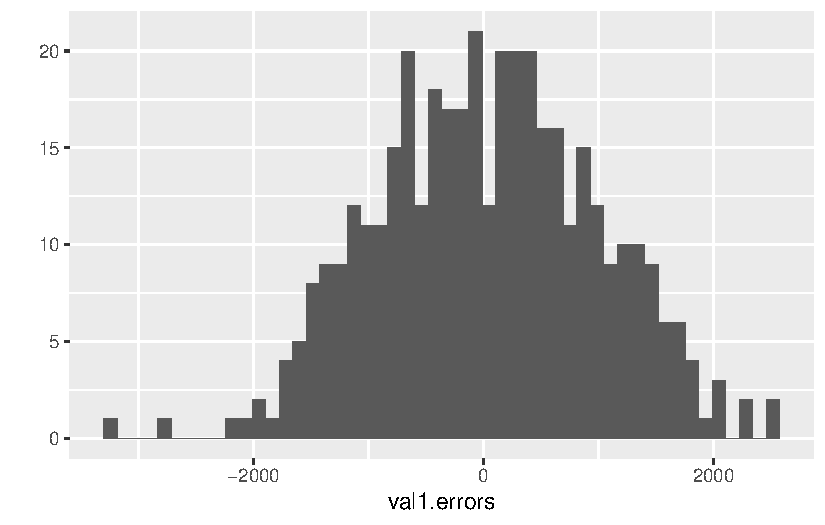
\includegraphics[keepaspectratio]{Group4_Final_Report_Project1_files/figure-pdf/unnamed-chunk-1-1.pdf}}

After running the testing for a few hundred rounds, we can plot the
values to see the mean and variance in accuracy. On average, the model
under predicts the value of income within a hundred dollars. However,
any specific training of the model can vary wildly, being within about 2
grand on average. Overall, we would say this is a fairlygood predictor
for a four-variable model. There are other angles to approach this a
question specifically tailored around how home neighborhood, but it
would require additional information not collected in this dataset

\subsection{Obstacles}\label{obstacles}

There were a few obstacles we ran into on question 3. One was how best
to evaluate predictive accuracy. We knew it needed to be tested across
multiple iterations to get an general accuracy, but I also wanted to
show the variance between each round. Ultimately we settled on giving
the overall mean prediction accuracy, as well as a histogram to
demonstrate the spread of predictions. The other issue we faced was in
adapting the question 3 ``rural'' value. As previously mentioned we
tried to find a solution to this issue but none of the information
within this dataset seemed to fulfill. The area zones are all 100,000
people at least, even if uneven numbers of people were surveyed from
each, and there was no variables directly measuring population density
or that could be used to determine it. Ultimately we just used area
zones as a separate predictive variable instead of specifically
``rural/urban'' comparison.

\subsection{Conclusions}\label{conclusions}

Our analysis indicates that income can be partially predicted using a
combination of demographic and socioeconomic factors, including age,
education, gender, and race. Education shows a strong positive
association with income, while age exhibits a nonlinear relationship,
with earnings increasing early in life and leveling off in later years.
Gender and race also demonstrate meaningful differences in income after
controlling for other variables. The multiple linear regression model
provides interpretable inference, though its overall explanatory power
is modest (R² ≈ 0.12), reflecting the inherent variability in income. To
complement this approach, LASSO regression was used to evaluate a
broader set of predictors and identify a more parsimonious subset of
variables. The LASSO results reinforce the importance of key demographic
and labor-related factors while reducing model complexity, highlighting
the value of combining interpretable models with regularization-based
variable selection.

The analysis shows that we can get a fairly accurate predictor of income
based on only a general area zone, commute time, vehicle type, and
availability of vehicles. Our predictor varied based on the
test/training split but was fairly accurate on average. Further research
with this model there are a lot of factors that could be considered such
as housing type and rural/suburban/urban living environment, but both of
these are outside the information captured by this dataset.

The analysis suggests that non-citizens in Oregon face substantially
higher odds of being uninsured (OR \textasciitilde{} 4.6 vs U.S.-born
residents) even after adjusting for income, education, employment, and
other demographics, indicating a large and persistent coverage gap. This
gap is driven primarily by structural and legal eligibility barriers
rather than socioeconomic differences, with only modest contributions
from factors like education, employment, and age.

\subsection{Citations}\label{citations}

\begin{enumerate}
\def\labelenumi{\arabic{enumi}.}
\item
  U.S. Census Bureau. (2026). 2020--2024 American Community Survey
  5-year Public Use Microdata Sample (PUMS). U.S. Department of
  Commerce. https://www.census.gov/programs-surveys/acs/microdata.html
\item
  Mason, H., \& Wiggins, C. (2010). A Taxonomy of Data Science.
  (Archived manuscript / teaching document). Accessed on 4/10/2026
  https://introdatasci.dlilab.com/pdf/A\_Taxonomy\_of\_Data\_Science.pdf
\end{enumerate}

\subsection{Appendix}\label{appendix}

\begin{Shaded}
\begin{Highlighting}[]
\NormalTok{knitr}\SpecialCharTok{::}\NormalTok{opts\_chunk}\SpecialCharTok{$}\FunctionTok{set}\NormalTok{(}
  \AttributeTok{warning =} \ConstantTok{FALSE}\NormalTok{,}
  \AttributeTok{message =} \ConstantTok{FALSE}\NormalTok{)}
\CommentTok{\#install.packages("ggfortify")}
\CommentTok{\#install.packages("kableExtra")}

\FunctionTok{library}\NormalTok{(tidyverse)}
\FunctionTok{library}\NormalTok{(patchwork)}
\FunctionTok{library}\NormalTok{(ggplot2)}
\FunctionTok{library}\NormalTok{(ggfortify)}
\FunctionTok{library}\NormalTok{(glmnet)}
\FunctionTok{library}\NormalTok{(faraway)}
\FunctionTok{library}\NormalTok{(car)}
\FunctionTok{library}\NormalTok{(gt)}
\FunctionTok{library}\NormalTok{(scales)}
\FunctionTok{library}\NormalTok{(survey)}
\FunctionTok{library}\NormalTok{(kableExtra)}
\CommentTok{\# reticulate::virtualenv\_create("r{-}reticulate")}
\CommentTok{\# reticulate::virtualenv\_install("r{-}reticulate", c("requests", "pandas"))}
\CommentTok{\# file.edit("\textasciitilde{}/.Rprofile")}
\CommentTok{\# add in this }
\CommentTok{\# Sys.setenv(RETICULATE\_PYTHON\_ENV = "r{-}reticulate")}
\CommentTok{\# run the following restart the python session if needed}
\CommentTok{\# reticulate::py\_run\_string("import gc; gc.collect()")}
\NormalTok{import requests}
\NormalTok{import json}
\NormalTok{from pathlib import Path}

\NormalTok{METADATA\_PATH }\OtherTok{=} \FunctionTok{Path}\NormalTok{(}\StringTok{"data/pums\_variables\_metadata.json"}\NormalTok{)}

\NormalTok{variables }\OtherTok{=}\NormalTok{ [ }\CommentTok{\# added POBP, JWTRNS, NRC}
    \StringTok{"WAGP"}\NormalTok{, }\StringTok{"PINCP"}\NormalTok{, }\StringTok{"PERNP"}\NormalTok{, }\StringTok{"POVPIP"}\NormalTok{, }\StringTok{"HICOV"}\NormalTok{, }\StringTok{"ESR"}\NormalTok{,}
    \StringTok{"AGEP"}\NormalTok{, }\StringTok{"SEX"}\NormalTok{, }\StringTok{"RAC1P"}\NormalTok{, }\StringTok{"HISP"}\NormalTok{, }\StringTok{"CIT"}\NormalTok{, }\StringTok{"YOEP"}\NormalTok{, }\StringTok{"MAR"}\NormalTok{, }\StringTok{"RELSHIPP"}\NormalTok{,}
    \StringTok{"POBP"}\NormalTok{, }\StringTok{"SCHL"}\NormalTok{, }\StringTok{"FOD1P"}\NormalTok{, }\StringTok{"SCH"}\NormalTok{, }\StringTok{"COW"}\NormalTok{, }\StringTok{"WKHP"}\NormalTok{, }\StringTok{"WKWN"}\NormalTok{, }\StringTok{"NAICSP"}\NormalTok{, }\StringTok{"OCCP"}\NormalTok{, }
    \StringTok{"WRK"}\NormalTok{, }\StringTok{"JWMNP"}\NormalTok{, }\StringTok{"JWTRNS"}\NormalTok{, }\StringTok{"PUMA"}\NormalTok{, }\StringTok{"MIG"}\NormalTok{, }\StringTok{"MIGSP"}\NormalTok{, }\StringTok{"POWSP"}\NormalTok{,}
    \StringTok{"DIS"}\NormalTok{, }\StringTok{"DPHY"}\NormalTok{, }\StringTok{"DREM"}\NormalTok{, }\StringTok{"DEAR"}\NormalTok{, }\StringTok{"DEYE"}\NormalTok{,}\StringTok{"HINCP"}\NormalTok{, }\StringTok{"HHT"}\NormalTok{, }\StringTok{"TEN"}\NormalTok{, }\StringTok{"VEH"}\NormalTok{,}
    \StringTok{"NRC"}\NormalTok{, }\StringTok{"RETP"}\NormalTok{, }\StringTok{"SSP"}\NormalTok{, }\StringTok{"SSIP"}\NormalTok{, }\StringTok{"PAP"}\NormalTok{, }\StringTok{"SEMP"}\NormalTok{,}
    \StringTok{"PWGTP"}\NormalTok{, }\StringTok{"ADJINC"}\NormalTok{,}
\NormalTok{]}

\NormalTok{BASE\_URL }\OtherTok{=} \StringTok{"https://api.census.gov/data/2024/acs/acs1/pums/variables/\{\}.json"}

\ControlFlowTok{if} \FunctionTok{METADATA\_PATH.exists}\NormalTok{()}\SpecialCharTok{:}
    \FunctionTok{print}\NormalTok{(f}\StringTok{"Loading metadata from cache: \{METADATA\_PATH\}"}\NormalTok{)}
\NormalTok{    with }\FunctionTok{open}\NormalTok{(METADATA\_PATH) as f}\SpecialCharTok{:}
\NormalTok{        metadata }\OtherTok{=} \FunctionTok{json.load}\NormalTok{(f)}
\ControlFlowTok{else}\SpecialCharTok{:}
    \FunctionTok{print}\NormalTok{(}\StringTok{"Fetching variable metadata from Census API..."}\NormalTok{)}
    \FunctionTok{METADATA\_PATH.parent.mkdir}\NormalTok{(}\AttributeTok{parents=}\NormalTok{True, }\AttributeTok{exist\_ok=}\NormalTok{True)}
\NormalTok{    metadata }\OtherTok{=}\NormalTok{ \{\}}

    \ControlFlowTok{for}\NormalTok{ var }\ControlFlowTok{in}\NormalTok{ variables}\SpecialCharTok{:}
\NormalTok{        response }\OtherTok{=} \FunctionTok{requests.get}\NormalTok{(}\FunctionTok{BASE\_URL.format}\NormalTok{(var), }\AttributeTok{timeout=}\DecValTok{30}\NormalTok{)}
        \ControlFlowTok{if}\NormalTok{ response.status\_code }\SpecialCharTok{==} \DecValTok{200}\SpecialCharTok{:}
\NormalTok{            metadata[var] }\OtherTok{=} \FunctionTok{response.json}\NormalTok{()}
            \FunctionTok{print}\NormalTok{(f}\StringTok{"  OK: \{var\}"}\NormalTok{)}
        \ControlFlowTok{else}\SpecialCharTok{:}
            \FunctionTok{print}\NormalTok{(f}\StringTok{"  FAILED: \{var\} — \{response.status\_code\}"}\NormalTok{)}

\NormalTok{    with }\FunctionTok{open}\NormalTok{(METADATA\_PATH, }\StringTok{"w"}\NormalTok{) as f}\SpecialCharTok{:}
        \FunctionTok{json.dump}\NormalTok{(metadata, f, }\AttributeTok{indent=}\DecValTok{2}\NormalTok{)}

    \FunctionTok{print}\NormalTok{(f}\StringTok{"}\SpecialCharTok{\textbackslash{}n}\StringTok{Saved metadata for \{len(metadata)\} variables to \{METADATA\_PATH\}"}\NormalTok{)}

\CommentTok{\# Preview one variable}
\FunctionTok{print}\NormalTok{(}\FunctionTok{json.dumps}\NormalTok{(}\FunctionTok{metadata.get}\NormalTok{(}\StringTok{"WAGP"}\NormalTok{, \{\}), }\AttributeTok{indent=}\DecValTok{2}\NormalTok{))}
\CommentTok{\# {-}{-}{-} Scrub Start {-}{-}{-}}

\NormalTok{import requests}
\NormalTok{import pandas as pd}
\NormalTok{from pathlib import Path}

\NormalTok{API\_KEY }\OtherTok{=} \StringTok{"a8f34453c39e419470f405353250f662a508d821"}
\NormalTok{YEAR }\OtherTok{=} \DecValTok{2024}
\NormalTok{STATE }\OtherTok{=} \StringTok{"41"}
\NormalTok{CACHE\_PATH }\OtherTok{=} \FunctionTok{Path}\NormalTok{(}\StringTok{"data/pums\_oregon\_2024.csv"}\NormalTok{)}

\NormalTok{variables }\OtherTok{=}\NormalTok{ [}
    \CommentTok{\# Outcomes}
    \StringTok{"WAGP"}\NormalTok{, }\StringTok{"PINCP"}\NormalTok{, }\StringTok{"PERNP"}\NormalTok{, }\StringTok{"POVPIP"}\NormalTok{, }\StringTok{"HICOV"}\NormalTok{, }\StringTok{"ESR"}\NormalTok{,}
    \CommentTok{\# Core demographics}
    \StringTok{"AGEP"}\NormalTok{, }\StringTok{"SEX"}\NormalTok{, }\StringTok{"RAC1P"}\NormalTok{, }\StringTok{"HISP"}\NormalTok{, }\StringTok{"CIT"}\NormalTok{, }\StringTok{"YOEP"}\NormalTok{, }\StringTok{"MAR"}\NormalTok{, }\StringTok{"RELSHIPP"}\NormalTok{,}
    \StringTok{"POBP"}\NormalTok{,                                                       }\CommentTok{\# added POBP}
    \CommentTok{\# Education}
    \StringTok{"SCHL"}\NormalTok{, }\StringTok{"FOD1P"}\NormalTok{, }\StringTok{"SCH"}\NormalTok{,}
    \CommentTok{\# Labor market}
    \StringTok{"COW"}\NormalTok{, }\StringTok{"WKHP"}\NormalTok{, }\StringTok{"WKWN"}\NormalTok{, }\StringTok{"NAICSP"}\NormalTok{, }\StringTok{"OCCP"}\NormalTok{, }\StringTok{"WRK"}\NormalTok{, }\StringTok{"JWMNP"}\NormalTok{, }\StringTok{"JWTRNS"}\NormalTok{, }\CommentTok{\# added}
    \CommentTok{\# Geography}
    \StringTok{"PUMA"}\NormalTok{, }\StringTok{"MIG"}\NormalTok{, }\StringTok{"MIGSP"}\NormalTok{, }\StringTok{"POWSP"}\NormalTok{,}
    \CommentTok{\# Disability \& health}
    \StringTok{"DIS"}\NormalTok{, }\StringTok{"DPHY"}\NormalTok{, }\StringTok{"DREM"}\NormalTok{, }\StringTok{"DEAR"}\NormalTok{, }\StringTok{"DEYE"}\NormalTok{,}
    \CommentTok{\# Household context}
    \StringTok{"HINCP"}\NormalTok{, }\StringTok{"HHT"}\NormalTok{, }\StringTok{"TEN"}\NormalTok{, }\StringTok{"VEH"}\NormalTok{, }\StringTok{"NRC"}\NormalTok{,                            }\CommentTok{\# added NRC}
    \CommentTok{\# Income components}
    \StringTok{"RETP"}\NormalTok{, }\StringTok{"SSP"}\NormalTok{, }\StringTok{"SSIP"}\NormalTok{, }\StringTok{"PAP"}\NormalTok{, }\StringTok{"SEMP"}\NormalTok{,}
    \CommentTok{\# Weights \& adjustments}
    \StringTok{"PWGTP"}\NormalTok{, }\StringTok{"ADJINC"}\NormalTok{,}\StringTok{"NP"}\NormalTok{,}
\NormalTok{]}

\ControlFlowTok{if} \FunctionTok{CACHE\_PATH.exists}\NormalTok{()}\SpecialCharTok{:}
    \FunctionTok{print}\NormalTok{(f}\StringTok{"Loading from local cache: \{CACHE\_PATH\}"}\NormalTok{)}
\NormalTok{    pums }\OtherTok{=} \FunctionTok{pd.read\_csv}\NormalTok{(CACHE\_PATH, }\AttributeTok{low\_memory=}\NormalTok{False)}
    \FunctionTok{print}\NormalTok{(f}\StringTok{"Loaded: \{len(pums):,\} rows, \{pums.shape[1]\} columns"}\NormalTok{)}
\ControlFlowTok{else}\SpecialCharTok{:}
    \FunctionTok{print}\NormalTok{(f}\StringTok{"Cache not found — fetching from Census API..."}\NormalTok{)}
    \FunctionTok{CACHE\_PATH.parent.mkdir}\NormalTok{(}\AttributeTok{parents=}\NormalTok{True, }\AttributeTok{exist\_ok=}\NormalTok{True)}
\NormalTok{    url }\OtherTok{=}\NormalTok{ (}
\NormalTok{        f}\StringTok{"https://api.census.gov/data/\{YEAR\}/acs/acs5/pums"}
\NormalTok{        f}\StringTok{"?get=\{\textquotesingle{},\textquotesingle{}.join(variables)\}"}
\NormalTok{        f}\StringTok{"\&for=state:\{STATE\}"}
\NormalTok{        f}\StringTok{"\&key=\{API\_KEY\}"}
\NormalTok{    )}
\NormalTok{    response }\OtherTok{=} \FunctionTok{requests.get}\NormalTok{(url, }\AttributeTok{timeout=}\DecValTok{60}\NormalTok{)}
    \FunctionTok{print}\NormalTok{(f}\StringTok{"Status code: \{response.status\_code\}"}\NormalTok{)}
    \ControlFlowTok{if}\NormalTok{ response.status\_code }\SpecialCharTok{==} \DecValTok{200}\SpecialCharTok{:}
\NormalTok{        data }\OtherTok{=} \FunctionTok{response.json}\NormalTok{()}
\NormalTok{        pums }\OtherTok{=} \FunctionTok{pd.DataFrame}\NormalTok{(data[}\DecValTok{1}\SpecialCharTok{:}\NormalTok{], }\AttributeTok{columns=}\NormalTok{data[}\DecValTok{0}\NormalTok{])}
        \FunctionTok{pums.to\_csv}\NormalTok{(CACHE\_PATH, }\AttributeTok{index=}\NormalTok{False)}
        \FunctionTok{print}\NormalTok{(f}\StringTok{"Saved to \{CACHE\_PATH\}: \{len(pums):,\} rows, \{pums.shape[1]\} columns"}\NormalTok{)}
    \ControlFlowTok{else}\SpecialCharTok{:}
        \FunctionTok{print}\NormalTok{(f}\StringTok{"Error: \{response.text[:500]\}"}\NormalTok{)}
\NormalTok{pums }\OtherTok{\textless{}{-}} \FunctionTok{read\_csv}\NormalTok{(}\StringTok{"data/pums\_oregon\_2024.csv"}\NormalTok{, }\AttributeTok{show\_col\_types =} \ConstantTok{FALSE}\NormalTok{)}

\CommentTok{\#glimpse(pums)}
\NormalTok{pums\_clean }\OtherTok{\textless{}{-}}\NormalTok{ pums }\SpecialCharTok{|\textgreater{}}

  \CommentTok{\# {-}{-}{-} Remove group quarters records {-}{-}{-}}
  \FunctionTok{filter}\NormalTok{(HINCP }\SpecialCharTok{!=} \SpecialCharTok{{-}}\DecValTok{60000}\NormalTok{) }\SpecialCharTok{|\textgreater{}}

  \CommentTok{\# {-}{-}{-} Apply income adjustment factor {-}{-}{-}}
  \FunctionTok{mutate}\NormalTok{(}
    \FunctionTok{across}\NormalTok{(}\FunctionTok{c}\NormalTok{(WAGP, PINCP, PERNP, HINCP, RETP, SSP, SSIP, PAP, SEMP),}
           \SpecialCharTok{\textasciitilde{}}\NormalTok{ .x }\SpecialCharTok{*}\NormalTok{ ADJINC)}
\NormalTok{  ) }\SpecialCharTok{|\textgreater{}}

  \CommentTok{\# {-}{-}{-} Recode all N/A sentinels to NA {-}{-}{-}}
  \FunctionTok{mutate}\NormalTok{(}
    \CommentTok{\# Income vars: age{-}based N/A}
    \AttributeTok{WAGP   =} \FunctionTok{na\_if}\NormalTok{(WAGP,  }\SpecialCharTok{{-}}\DecValTok{1} \SpecialCharTok{*}\NormalTok{ ADJINC),}
    \AttributeTok{PERNP  =} \FunctionTok{na\_if}\NormalTok{(PERNP, }\SpecialCharTok{{-}}\DecValTok{10001} \SpecialCharTok{*}\NormalTok{ ADJINC),}
    \AttributeTok{PINCP  =} \FunctionTok{na\_if}\NormalTok{(PINCP, }\SpecialCharTok{{-}}\DecValTok{19999} \SpecialCharTok{*}\NormalTok{ ADJINC),}
    \AttributeTok{RETP   =} \FunctionTok{na\_if}\NormalTok{(RETP,  }\SpecialCharTok{{-}}\DecValTok{1} \SpecialCharTok{*}\NormalTok{ ADJINC),}
    \AttributeTok{SSP    =} \FunctionTok{na\_if}\NormalTok{(SSP,   }\SpecialCharTok{{-}}\DecValTok{1} \SpecialCharTok{*}\NormalTok{ ADJINC),}
    \AttributeTok{SSIP   =} \FunctionTok{na\_if}\NormalTok{(SSIP,  }\SpecialCharTok{{-}}\DecValTok{1} \SpecialCharTok{*}\NormalTok{ ADJINC),}
    \AttributeTok{PAP    =} \FunctionTok{na\_if}\NormalTok{(PAP,   }\SpecialCharTok{{-}}\DecValTok{1} \SpecialCharTok{*}\NormalTok{ ADJINC),}
    \AttributeTok{SEMP   =} \FunctionTok{na\_if}\NormalTok{(SEMP,  }\SpecialCharTok{{-}}\DecValTok{10001} \SpecialCharTok{*}\NormalTok{ ADJINC),}
    \CommentTok{\# Labor market: 0 = N/A (under 16 or did not work)}
    \AttributeTok{WKHP   =} \FunctionTok{na\_if}\NormalTok{(WKHP, }\DecValTok{0}\NormalTok{),}
    \AttributeTok{WKWN   =} \FunctionTok{na\_if}\NormalTok{(WKWN, }\DecValTok{0}\NormalTok{),}
    \AttributeTok{JWMNP  =} \FunctionTok{na\_if}\NormalTok{(JWMNP, }\DecValTok{0}\NormalTok{),}
    \CommentTok{\# Other sentinels}
    \AttributeTok{POVPIP =} \FunctionTok{na\_if}\NormalTok{(POVPIP, }\SpecialCharTok{{-}}\DecValTok{1}\NormalTok{),}
    \AttributeTok{ESR    =} \FunctionTok{na\_if}\NormalTok{(ESR, }\DecValTok{0}\NormalTok{),}
    \AttributeTok{YOEP   =} \FunctionTok{na\_if}\NormalTok{(YOEP, }\DecValTok{1937}\NormalTok{),}
    \AttributeTok{HHT    =} \FunctionTok{na\_if}\NormalTok{(HHT, }\DecValTok{0}\NormalTok{),}
    \AttributeTok{TEN    =} \FunctionTok{na\_if}\NormalTok{(TEN, }\DecValTok{0}\NormalTok{),}
    \AttributeTok{VEH    =} \FunctionTok{na\_if}\NormalTok{(VEH, }\SpecialCharTok{{-}}\DecValTok{1}\NormalTok{),}
    \AttributeTok{NRC    =} \FunctionTok{na\_if}\NormalTok{(NRC, }\SpecialCharTok{{-}}\DecValTok{1}\NormalTok{),}
    \AttributeTok{DPHY   =} \FunctionTok{na\_if}\NormalTok{(DPHY, }\DecValTok{0}\NormalTok{),}
    \AttributeTok{DREM   =} \FunctionTok{na\_if}\NormalTok{(DREM, }\DecValTok{0}\NormalTok{),}
    \AttributeTok{NP     =} \FunctionTok{na\_if}\NormalTok{(NP, }\DecValTok{0}\NormalTok{),}
    \CommentTok{\# Labor class and work status: 0 = N/A}
    \AttributeTok{COW    =} \FunctionTok{na\_if}\NormalTok{(COW, }\DecValTok{0}\NormalTok{),}
    \AttributeTok{WRK    =} \FunctionTok{na\_if}\NormalTok{(WRK, }\DecValTok{0}\NormalTok{),}
\NormalTok{  ) }\SpecialCharTok{|\textgreater{}}

  \CommentTok{\# {-}{-}{-} Recode binary vars to logical (1=Yes, 2=No) {-}{-}{-}}
  \FunctionTok{mutate}\NormalTok{(}
    \FunctionTok{across}\NormalTok{(}\FunctionTok{c}\NormalTok{(DPHY, DREM, DEAR, DEYE, DIS), }\SpecialCharTok{\textasciitilde{}}\NormalTok{ .x }\SpecialCharTok{==} \DecValTok{1}\NormalTok{),}
    \AttributeTok{HICOV =}\NormalTok{ HICOV }\SpecialCharTok{==} \DecValTok{1}\NormalTok{,}
\NormalTok{  ) }\SpecialCharTok{|\textgreater{}}

  \CommentTok{\# {-}{-}{-} Recode categorical vars as factors with labels from metadata {-}{-}{-}}
  \FunctionTok{mutate}\NormalTok{(}
    \AttributeTok{SEX =} \FunctionTok{factor}\NormalTok{(SEX, }\AttributeTok{levels =} \FunctionTok{c}\NormalTok{(}\DecValTok{1}\NormalTok{, }\DecValTok{2}\NormalTok{),}
                 \AttributeTok{labels =} \FunctionTok{c}\NormalTok{(}\StringTok{"Male"}\NormalTok{, }\StringTok{"Female"}\NormalTok{)),}

    \AttributeTok{RAC1P =} \FunctionTok{factor}\NormalTok{(RAC1P, }\AttributeTok{levels =} \DecValTok{1}\SpecialCharTok{:}\DecValTok{9}\NormalTok{,}
                   \AttributeTok{labels =} \FunctionTok{c}\NormalTok{(}\StringTok{"White alone"}\NormalTok{, }\StringTok{"Black or African American alone"}\NormalTok{,}
                              \StringTok{"American Indian alone"}\NormalTok{, }\StringTok{"Alaska Native alone"}\NormalTok{,}
                              \StringTok{"AIAN tribes specified"}\NormalTok{, }\StringTok{"Asian alone"}\NormalTok{,}
                              \StringTok{"Native Hawaiian and Other Pacific Islander alone"}\NormalTok{,}
                              \StringTok{"Some other race alone"}\NormalTok{, }\StringTok{"Two or More Races"}\NormalTok{)),}

    \AttributeTok{HISP\_binary =} \FunctionTok{factor}\NormalTok{(}\FunctionTok{if\_else}\NormalTok{(HISP }\SpecialCharTok{==} \StringTok{"01"}\NormalTok{, }\StringTok{"Not Hispanic"}\NormalTok{, }\StringTok{"Hispanic"}\NormalTok{)),}

    \AttributeTok{CIT =} \FunctionTok{factor}\NormalTok{(CIT, }\AttributeTok{levels =} \DecValTok{1}\SpecialCharTok{:}\DecValTok{5}\NormalTok{,}
                 \AttributeTok{labels =} \FunctionTok{c}\NormalTok{(}\StringTok{"Born in US"}\NormalTok{, }\StringTok{"Born in PR/territories"}\NormalTok{,}
                            \StringTok{"Born abroad of US citizen parent"}\NormalTok{,}
                            \StringTok{"Naturalized citizen"}\NormalTok{, }\StringTok{"Not a US citizen"}\NormalTok{)),}

    \AttributeTok{MAR =} \FunctionTok{factor}\NormalTok{(MAR, }\AttributeTok{levels =} \DecValTok{1}\SpecialCharTok{:}\DecValTok{5}\NormalTok{,}
                 \AttributeTok{labels =} \FunctionTok{c}\NormalTok{(}\StringTok{"Married"}\NormalTok{, }\StringTok{"Widowed"}\NormalTok{, }\StringTok{"Divorced"}\NormalTok{,}
                            \StringTok{"Separated"}\NormalTok{, }\StringTok{"Never married"}\NormalTok{)),}

    \AttributeTok{ESR =} \FunctionTok{factor}\NormalTok{(ESR, }\AttributeTok{levels =} \DecValTok{1}\SpecialCharTok{:}\DecValTok{6}\NormalTok{,}
                 \AttributeTok{labels =} \FunctionTok{c}\NormalTok{(}\StringTok{"Civilian employed at work"}\NormalTok{,}
                            \StringTok{"Civilian employed not at work"}\NormalTok{,}
                            \StringTok{"Unemployed"}\NormalTok{,}
                            \StringTok{"Armed Forces at work"}\NormalTok{,}
                            \StringTok{"Armed Forces not at work"}\NormalTok{,}
                            \StringTok{"Not in labor force"}\NormalTok{)),}

    \AttributeTok{SCH =} \FunctionTok{factor}\NormalTok{(SCH, }\AttributeTok{levels =} \DecValTok{1}\SpecialCharTok{:}\DecValTok{3}\NormalTok{,}
                 \AttributeTok{labels =} \FunctionTok{c}\NormalTok{(}\StringTok{"Not enrolled"}\NormalTok{, }\StringTok{"Public school"}\NormalTok{, }\StringTok{"Private school"}\NormalTok{)),}

    \AttributeTok{COW =} \FunctionTok{factor}\NormalTok{(COW, }\AttributeTok{levels =} \DecValTok{1}\SpecialCharTok{:}\DecValTok{9}\NormalTok{,}
                 \AttributeTok{labels =} \FunctionTok{c}\NormalTok{(}\StringTok{"Private for{-}profit"}\NormalTok{, }\StringTok{"Private nonprofit"}\NormalTok{,}
                            \StringTok{"Local govt"}\NormalTok{, }\StringTok{"State govt"}\NormalTok{, }\StringTok{"Federal govt"}\NormalTok{,}
                            \StringTok{"Self{-}emp incorporated"}\NormalTok{, }\StringTok{"Self{-}emp not incorporated"}\NormalTok{,}
                            \StringTok{"Working without pay"}\NormalTok{, }\StringTok{"Unemployed last 5 years"}\NormalTok{)),}

    \AttributeTok{MIG =} \FunctionTok{factor}\NormalTok{(MIG, }\AttributeTok{levels =} \DecValTok{1}\SpecialCharTok{:}\DecValTok{3}\NormalTok{,}
                 \AttributeTok{labels =} \FunctionTok{c}\NormalTok{(}\StringTok{"Same house"}\NormalTok{, }\StringTok{"Outside US"}\NormalTok{, }\StringTok{"Different house in US"}\NormalTok{)),}

    \AttributeTok{HHT =} \FunctionTok{factor}\NormalTok{(HHT, }\AttributeTok{levels =} \DecValTok{1}\SpecialCharTok{:}\DecValTok{7}\NormalTok{,}
                 \AttributeTok{labels =} \FunctionTok{c}\NormalTok{(}\StringTok{"Married couple household"}\NormalTok{,}
                            \StringTok{"Other family: male householder no spouse"}\NormalTok{,}
                            \StringTok{"Other family: female householder no spouse"}\NormalTok{,}
                            \StringTok{"Nonfamily: male householder living alone"}\NormalTok{,}
                            \StringTok{"Nonfamily: male householder not living alone"}\NormalTok{,}
                            \StringTok{"Nonfamily: female householder living alone"}\NormalTok{,}
                            \StringTok{"Nonfamily: female householder not living alone"}\NormalTok{)),}

    \AttributeTok{TEN =} \FunctionTok{factor}\NormalTok{(TEN, }\AttributeTok{levels =} \DecValTok{1}\SpecialCharTok{:}\DecValTok{4}\NormalTok{,}
                 \AttributeTok{labels =} \FunctionTok{c}\NormalTok{(}\StringTok{"Owned with mortgage"}\NormalTok{, }\StringTok{"Owned free and clear"}\NormalTok{,}
                            \StringTok{"Rented"}\NormalTok{, }\StringTok{"Occupied without payment"}\NormalTok{)),}

    \AttributeTok{WRK =} \FunctionTok{factor}\NormalTok{(WRK, }\AttributeTok{levels =} \DecValTok{1}\SpecialCharTok{:}\DecValTok{2}\NormalTok{,}
                 \AttributeTok{labels =} \FunctionTok{c}\NormalTok{(}\StringTok{"Worked last week"}\NormalTok{, }\StringTok{"Did not work last week"}\NormalTok{)),}

    \AttributeTok{JWTRNS =} \FunctionTok{factor}\NormalTok{(JWTRNS, }\AttributeTok{levels =} \DecValTok{0}\SpecialCharTok{:}\DecValTok{12}\NormalTok{,}
                    \AttributeTok{labels =} \FunctionTok{c}\NormalTok{(}\StringTok{"N/A"}\NormalTok{, }\StringTok{"Car truck or van"}\NormalTok{, }\StringTok{"Bus"}\NormalTok{,}
                               \StringTok{"Subway or elevated rail"}\NormalTok{,}
                               \StringTok{"Long{-}distance train or commuter rail"}\NormalTok{,}
                               \StringTok{"Light rail streetcar or trolley"}\NormalTok{,}
                               \StringTok{"Ferryboat"}\NormalTok{, }\StringTok{"Taxi or ride{-}hailing"}\NormalTok{,}
                               \StringTok{"Motorcycle"}\NormalTok{, }\StringTok{"Bicycle"}\NormalTok{, }\StringTok{"Walked"}\NormalTok{,}
                               \StringTok{"Worked from home"}\NormalTok{, }\StringTok{"Other method"}\NormalTok{)),}

    \AttributeTok{POBP\_binary =} \FunctionTok{factor}\NormalTok{(}\FunctionTok{case\_when}\NormalTok{(}
      \FunctionTok{as.numeric}\NormalTok{(POBP) }\SpecialCharTok{\textless{}=} \DecValTok{56}  \SpecialCharTok{\textasciitilde{}} \StringTok{"Born in US"}\NormalTok{,}
      \FunctionTok{as.numeric}\NormalTok{(POBP) }\SpecialCharTok{==} \DecValTok{72}  \SpecialCharTok{\textasciitilde{}} \StringTok{"Born in PR/territories"}\NormalTok{,}
      \ConstantTok{TRUE}                    \SpecialCharTok{\textasciitilde{}} \StringTok{"Foreign born"}
\NormalTok{    )),}
\NormalTok{  ) }\SpecialCharTok{|\textgreater{}}

  \CommentTok{\# {-}{-}{-} Drop redundant/replaced columns {-}{-}{-}}
  \FunctionTok{select}\NormalTok{(}\SpecialCharTok{{-}}\NormalTok{ADJINC, }\SpecialCharTok{{-}}\NormalTok{HISP, }\SpecialCharTok{{-}}\NormalTok{POBP, }\SpecialCharTok{{-}}\NormalTok{state) }\SpecialCharTok{|\textgreater{}}

  \CommentTok{\# {-}{-}{-} Ensure valid person weight {-}{-}{-}}
  \FunctionTok{filter}\NormalTok{(}\SpecialCharTok{!}\FunctionTok{is.na}\NormalTok{(PWGTP), PWGTP }\SpecialCharTok{\textgreater{}} \DecValTok{0}\NormalTok{)}

\CommentTok{\#glimpse(pums\_clean)}
\CommentTok{\# {-}{-}{-} Note {-}{-}{-}}
\CommentTok{\# after data pull and scrub in Python from the API}
\CommentTok{\# the following was a proposed EDA method}
\CommentTok{\# the group did chose to work in a different direction for EDA}
\CommentTok{\# we have left if here for possible future use}

\FunctionTok{library}\NormalTok{(tidyverse)}
\FunctionTok{library}\NormalTok{(skimr)}

\CommentTok{\# 1. overall summary}
\CommentTok{\#skim(pums\_clean)}
\CommentTok{\# Wages among earners only}

\CommentTok{\# Log wages}

\CommentTok{\# Total personal income}
\CommentTok{\# Q1/Q3: wage statistics by key groups}

\CommentTok{\# Q2: health insurance coverage rate}

\CommentTok{\# Q2: uninsured rate by citizenship}
\CommentTok{\# {-}{-}{-} End EDA proposal {-}{-}{-}}

\FunctionTok{library}\NormalTok{(corrr)}
\NormalTok{p1 }\OtherTok{\textless{}{-}}\FunctionTok{ggplot}\NormalTok{(}\AttributeTok{data =}\NormalTok{ pums\_clean, }\FunctionTok{aes}\NormalTok{(}\AttributeTok{x =}\NormalTok{ PINCP)) }\SpecialCharTok{+}
  \FunctionTok{geom\_histogram}\NormalTok{(}\AttributeTok{binwidth =} \DecValTok{30000}\NormalTok{) }\SpecialCharTok{+} 
  \FunctionTok{labs}\NormalTok{(}
    \AttributeTok{y =} \StringTok{"Count"}\NormalTok{,}
    \AttributeTok{x =} \StringTok{"Personal Income"}
\NormalTok{  )}


\NormalTok{p2 }\OtherTok{\textless{}{-}}\FunctionTok{ggplot}\NormalTok{(}\AttributeTok{data =}\NormalTok{ pums\_clean, }\FunctionTok{aes}\NormalTok{(}\AttributeTok{x =} \FunctionTok{log}\NormalTok{(pums\_clean}\SpecialCharTok{$}\NormalTok{PINCP)}\SpecialCharTok{+}\DecValTok{1}\NormalTok{)) }\SpecialCharTok{+}
  \FunctionTok{geom\_histogram}\NormalTok{(}\AttributeTok{binwidth =} \DecValTok{1}\NormalTok{) }\SpecialCharTok{+} 
  \FunctionTok{labs}\NormalTok{(}
    \AttributeTok{y =} \StringTok{"Count"}\NormalTok{,}
    \AttributeTok{x =} \StringTok{"log() of Personal Income"}
\NormalTok{  )}

\NormalTok{p1 }\SpecialCharTok{+}\NormalTok{ p2 }\SpecialCharTok{+} \FunctionTok{plot\_layout}\NormalTok{(}\AttributeTok{ncol =} \DecValTok{2}\NormalTok{)}
\CommentTok{\# This takes a long time to run, adding if statement}
\CommentTok{\# so it only gets run when needed.}
\NormalTok{outfile }\OtherTok{\textless{}{-}} \StringTok{"./eda{-}incomevage{-}plot.png"}

\ControlFlowTok{if}\NormalTok{ (}\SpecialCharTok{!}\FunctionTok{file.exists}\NormalTok{(outfile)) \{}
\NormalTok{  incomevage\_plot }\OtherTok{\textless{}{-}} \FunctionTok{ggplot}\NormalTok{(pums\_clean, }\FunctionTok{aes}\NormalTok{(}\AttributeTok{x =}\NormalTok{ AGEP, }\AttributeTok{y =}\NormalTok{ PINCP)) }\SpecialCharTok{+}
    \FunctionTok{geom\_point}\NormalTok{(}\AttributeTok{alpha =} \FloatTok{0.2}\NormalTok{) }\SpecialCharTok{+}
    \FunctionTok{geom\_smooth}\NormalTok{(}\AttributeTok{method =} \StringTok{"loess"}\NormalTok{) }\SpecialCharTok{+}
    \FunctionTok{scale\_y\_continuous}\NormalTok{(}\AttributeTok{labels =} \FunctionTok{label\_number}\NormalTok{()) }\SpecialCharTok{+}
    \FunctionTok{labs}\NormalTok{(}\AttributeTok{title =} \StringTok{"Census Data: Personal Income vs Age"}\NormalTok{)}
    \FunctionTok{ggsave}\NormalTok{(outfile, }\AttributeTok{plot =}\NormalTok{ incomevage\_plot, }\AttributeTok{width =} \DecValTok{10}\NormalTok{, }\AttributeTok{height =} \DecValTok{6}\NormalTok{, }\AttributeTok{dpi =} \DecValTok{300}\NormalTok{)}
\NormalTok{\}}
\CommentTok{\# This takes a long time to run, adding if statement}
\CommentTok{\# so it only gets run when needed.}
\NormalTok{outfile }\OtherTok{\textless{}{-}} \StringTok{"./eda{-}incomeved{-}plot.png"}

\ControlFlowTok{if}\NormalTok{ (}\SpecialCharTok{!}\FunctionTok{file.exists}\NormalTok{(outfile)) \{}
\NormalTok{  incomeved\_plot }\OtherTok{\textless{}{-}} \FunctionTok{ggplot}\NormalTok{(pums\_clean, }\FunctionTok{aes}\NormalTok{(}\AttributeTok{x =}\NormalTok{ SCHL, }\AttributeTok{y =}\NormalTok{ PINCP)) }\SpecialCharTok{+}
    \FunctionTok{geom\_point}\NormalTok{(}\AttributeTok{alpha =} \FloatTok{0.2}\NormalTok{) }\SpecialCharTok{+}
    \FunctionTok{geom\_smooth}\NormalTok{(}\AttributeTok{method =} \StringTok{"loess"}\NormalTok{) }\SpecialCharTok{+}
    \FunctionTok{scale\_y\_continuous}\NormalTok{(}\AttributeTok{labels =} \FunctionTok{label\_number}\NormalTok{()) }\SpecialCharTok{+}
    \FunctionTok{labs}\NormalTok{(}\AttributeTok{title =} \StringTok{"Income vs Education"}\NormalTok{, }\AttributeTok{x =} \StringTok{"Years of School (Education)"}\NormalTok{, }\AttributeTok{y =} \StringTok{"Income"}\NormalTok{)}
  \FunctionTok{ggsave}\NormalTok{(outfile, }\AttributeTok{plot =}\NormalTok{ incomeved\_plot, }\AttributeTok{width =} \DecValTok{10}\NormalTok{, }\AttributeTok{height =} \DecValTok{6}\NormalTok{, }\AttributeTok{dpi =} \DecValTok{300}\NormalTok{)}
\NormalTok{\}}
\FunctionTok{ggplot}\NormalTok{(pums\_clean, }\FunctionTok{aes}\NormalTok{(}\AttributeTok{x =} \FunctionTok{factor}\NormalTok{(SEX), }\AttributeTok{y =}\NormalTok{ PINCP)) }\SpecialCharTok{+}
  \FunctionTok{geom\_boxplot}\NormalTok{() }\SpecialCharTok{+}
  \FunctionTok{coord\_cartesian}\NormalTok{(}\AttributeTok{ylim =} \FunctionTok{c}\NormalTok{(}\DecValTok{0}\NormalTok{, }\DecValTok{200000}\NormalTok{)) }\SpecialCharTok{+}
  \FunctionTok{scale\_x\_discrete}\NormalTok{(}\AttributeTok{labels =} \FunctionTok{c}\NormalTok{(}\StringTok{"Male"}\NormalTok{, }\StringTok{"Female"}\NormalTok{)) }\SpecialCharTok{+}
  \FunctionTok{labs}\NormalTok{(}
    \AttributeTok{title =} \StringTok{"Income by Gender"}\NormalTok{,}
    \AttributeTok{x =} \StringTok{"Gender"}\NormalTok{,}
    \AttributeTok{y =} \StringTok{"Income"}
\NormalTok{  ) }\SpecialCharTok{+}
  \FunctionTok{theme\_minimal}\NormalTok{()}
\FunctionTok{ggsave}\NormalTok{(}\StringTok{"./eda{-}incomevgender{-}plot.png"}\NormalTok{, }\AttributeTok{width =} \DecValTok{10}\NormalTok{, }\AttributeTok{height =} \DecValTok{6}\NormalTok{, }\AttributeTok{dpi =} \DecValTok{300}\NormalTok{)}
\FunctionTok{ggplot}\NormalTok{(pums\_clean, }\FunctionTok{aes}\NormalTok{(}\AttributeTok{x =} \FunctionTok{factor}\NormalTok{(RAC1P), }\AttributeTok{y =}\NormalTok{ PINCP)) }\SpecialCharTok{+}
  \FunctionTok{geom\_boxplot}\NormalTok{() }\SpecialCharTok{+}
  \FunctionTok{coord\_cartesian}\NormalTok{(}\AttributeTok{ylim =} \FunctionTok{c}\NormalTok{(}\DecValTok{0}\NormalTok{, }\DecValTok{200000}\NormalTok{)) }\SpecialCharTok{+}
  \FunctionTok{labs}\NormalTok{(}
    \AttributeTok{title =} \StringTok{"Income by Race"}\NormalTok{,}
    \AttributeTok{x =} \StringTok{"Race"}\NormalTok{,}
    \AttributeTok{y =} \StringTok{"Income"}
\NormalTok{  ) }\SpecialCharTok{+}
  \FunctionTok{theme\_minimal}\NormalTok{() }\SpecialCharTok{+}
  \FunctionTok{theme}\NormalTok{(}\AttributeTok{axis.text.x =} \FunctionTok{element\_text}\NormalTok{(}\AttributeTok{angle =} \DecValTok{45}\NormalTok{, }\AttributeTok{hjust =} \DecValTok{1}\NormalTok{)) }\SpecialCharTok{+}
  \FunctionTok{scale\_x\_discrete}\NormalTok{(}\AttributeTok{labels =} \FunctionTok{c}\NormalTok{(}
    \StringTok{"White alone"} \OtherTok{=} \StringTok{"White"}\NormalTok{,}
    \StringTok{"Black or African American alone"} \OtherTok{=} \StringTok{"Black"}\NormalTok{,}
    \StringTok{"American Indian alone"} \OtherTok{=} \StringTok{"AIAN"}\NormalTok{,}
    \StringTok{"Alaska Native alone"} \OtherTok{=} \StringTok{"Alaska Nat."}\NormalTok{,}
    \StringTok{"AIAN w/ tribes specified"} \OtherTok{=} \StringTok{"AIAN (tribe)"}\NormalTok{,}
    \StringTok{"Asian alone"} \OtherTok{=} \StringTok{"Asian"}\NormalTok{,}
    \StringTok{"Native Hawaiian and Other Pacific Islander alone"} \OtherTok{=} \StringTok{"NHPI"}\NormalTok{,}
    \StringTok{"Some other race alone"} \OtherTok{=} \StringTok{"Other"}\NormalTok{,}
    \StringTok{"Two or More Races"} \OtherTok{=} \StringTok{"Two or More Races"}
\NormalTok{  ))}
\FunctionTok{ggsave}\NormalTok{(}\StringTok{"./eda{-}incomevrace{-}plot.png"}\NormalTok{, }\AttributeTok{width =} \DecValTok{10}\NormalTok{, }\AttributeTok{height =} \DecValTok{6}\NormalTok{, }\AttributeTok{dpi =} \DecValTok{300}\NormalTok{)}
\CommentTok{\# build OCCP group lookup on distinct codes only}
\NormalTok{occp\_groups }\OtherTok{\textless{}{-}}\NormalTok{ pums\_clean }\SpecialCharTok{|\textgreater{}}
  \FunctionTok{filter}\NormalTok{(OCCP }\SpecialCharTok{!=} \StringTok{"N"}\NormalTok{, }\SpecialCharTok{!}\FunctionTok{is.na}\NormalTok{(OCCP)) }\SpecialCharTok{|\textgreater{}}
  \FunctionTok{distinct}\NormalTok{(OCCP) }\SpecialCharTok{|\textgreater{}}
  \FunctionTok{mutate}\NormalTok{(}
    \AttributeTok{OCCP\_group =} \FunctionTok{case\_when}\NormalTok{(}
      \FunctionTok{between}\NormalTok{(}\FunctionTok{suppressWarnings}\NormalTok{(}\FunctionTok{as.numeric}\NormalTok{(OCCP)), }\DecValTok{10}\NormalTok{,   }\DecValTok{960}\NormalTok{)  }\SpecialCharTok{\textasciitilde{}} \StringTok{"High coverage"}\NormalTok{,}
      \FunctionTok{between}\NormalTok{(}\FunctionTok{suppressWarnings}\NormalTok{(}\FunctionTok{as.numeric}\NormalTok{(OCCP)), }\DecValTok{1005}\NormalTok{, }\DecValTok{2555}\NormalTok{) }\SpecialCharTok{\textasciitilde{}} \StringTok{"High coverage"}\NormalTok{,}
      \FunctionTok{between}\NormalTok{(}\FunctionTok{suppressWarnings}\NormalTok{(}\FunctionTok{as.numeric}\NormalTok{(OCCP)), }\DecValTok{3000}\NormalTok{, }\DecValTok{3550}\NormalTok{) }\SpecialCharTok{\textasciitilde{}} \StringTok{"High coverage"}\NormalTok{,}
      \FunctionTok{between}\NormalTok{(}\FunctionTok{suppressWarnings}\NormalTok{(}\FunctionTok{as.numeric}\NormalTok{(OCCP)), }\DecValTok{2600}\NormalTok{, }\DecValTok{2920}\NormalTok{) }\SpecialCharTok{\textasciitilde{}} \StringTok{"Variable coverage"}\NormalTok{,}
      \FunctionTok{between}\NormalTok{(}\FunctionTok{suppressWarnings}\NormalTok{(}\FunctionTok{as.numeric}\NormalTok{(OCCP)), }\DecValTok{3600}\NormalTok{, }\DecValTok{3655}\NormalTok{) }\SpecialCharTok{\textasciitilde{}} \StringTok{"Variable coverage"}\NormalTok{,}
      \FunctionTok{between}\NormalTok{(}\FunctionTok{suppressWarnings}\NormalTok{(}\FunctionTok{as.numeric}\NormalTok{(OCCP)), }\DecValTok{4330}\NormalTok{, }\DecValTok{5940}\NormalTok{) }\SpecialCharTok{\textasciitilde{}} \StringTok{"Variable coverage"}\NormalTok{,}
      \FunctionTok{between}\NormalTok{(}\FunctionTok{suppressWarnings}\NormalTok{(}\FunctionTok{as.numeric}\NormalTok{(OCCP)), }\DecValTok{4000}\NormalTok{, }\DecValTok{4255}\NormalTok{) }\SpecialCharTok{\textasciitilde{}} \StringTok{"Low coverage"}\NormalTok{,}
      \FunctionTok{between}\NormalTok{(}\FunctionTok{suppressWarnings}\NormalTok{(}\FunctionTok{as.numeric}\NormalTok{(OCCP)), }\DecValTok{6005}\NormalTok{, }\DecValTok{6130}\NormalTok{) }\SpecialCharTok{\textasciitilde{}} \StringTok{"Low coverage"}\NormalTok{,}
      \FunctionTok{between}\NormalTok{(}\FunctionTok{suppressWarnings}\NormalTok{(}\FunctionTok{as.numeric}\NormalTok{(OCCP)), }\DecValTok{6200}\NormalTok{, }\DecValTok{8990}\NormalTok{) }\SpecialCharTok{\textasciitilde{}} \StringTok{"Low coverage"}\NormalTok{,}
      \FunctionTok{between}\NormalTok{(}\FunctionTok{suppressWarnings}\NormalTok{(}\FunctionTok{as.numeric}\NormalTok{(OCCP)), }\DecValTok{9005}\NormalTok{, }\DecValTok{9760}\NormalTok{) }\SpecialCharTok{\textasciitilde{}} \StringTok{"Low coverage"}\NormalTok{,}
      \FunctionTok{between}\NormalTok{(}\FunctionTok{suppressWarnings}\NormalTok{(}\FunctionTok{as.numeric}\NormalTok{(OCCP)), }\DecValTok{3700}\NormalTok{, }\DecValTok{3960}\NormalTok{) }\SpecialCharTok{\textasciitilde{}} \StringTok{"Military \& Protective"}\NormalTok{,}
      \FunctionTok{between}\NormalTok{(}\FunctionTok{suppressWarnings}\NormalTok{(}\FunctionTok{as.numeric}\NormalTok{(OCCP)), }\DecValTok{9800}\NormalTok{, }\DecValTok{9830}\NormalTok{) }\SpecialCharTok{\textasciitilde{}} \StringTok{"Military \& Protective"}\NormalTok{,}
      \ConstantTok{TRUE}                                                     \SpecialCharTok{\textasciitilde{}} \StringTok{"Variable coverage"}
\NormalTok{    ),}
    \AttributeTok{OCCP\_group =} \FunctionTok{factor}\NormalTok{(OCCP\_group,}
                        \AttributeTok{levels =} \FunctionTok{c}\NormalTok{(}\StringTok{"High coverage"}\NormalTok{, }\StringTok{"Variable coverage"}\NormalTok{,}
                                   \StringTok{"Low coverage"}\NormalTok{, }\StringTok{"Military \& Protective"}\NormalTok{))}
\NormalTok{  )}

\CommentTok{\# check}
\FunctionTok{cat}\NormalTok{(}\StringTok{"Distinct OCCP codes mapped:"}\NormalTok{, }\FunctionTok{nrow}\NormalTok{(occp\_groups), }\StringTok{"}\SpecialCharTok{\textbackslash{}n}\StringTok{"}\NormalTok{)}
\FunctionTok{count}\NormalTok{(occp\_groups, OCCP\_group)}
\NormalTok{pums\_q2 }\OtherTok{\textless{}{-}}\NormalTok{ pums\_clean }\SpecialCharTok{|\textgreater{}}
  \FunctionTok{left\_join}\NormalTok{(occp\_groups, }\AttributeTok{by =} \StringTok{"OCCP"}\NormalTok{) }\SpecialCharTok{|\textgreater{}}
  \FunctionTok{mutate}\NormalTok{(}
    \CommentTok{\# response: uninsured}
    \AttributeTok{UNINSURED =} \FunctionTok{as.integer}\NormalTok{(}\SpecialCharTok{!}\NormalTok{HICOV),}

    \CommentTok{\# education collapsed to degree attainment groups}
    \AttributeTok{SCHL\_group =} \FunctionTok{case\_when}\NormalTok{(}
\NormalTok{      SCHL }\SpecialCharTok{\textless{}=} \DecValTok{15}           \SpecialCharTok{\textasciitilde{}} \StringTok{"Less than high school"}\NormalTok{,}
\NormalTok{      SCHL }\SpecialCharTok{\%in\%} \FunctionTok{c}\NormalTok{(}\DecValTok{16}\NormalTok{, }\DecValTok{17}\NormalTok{) }\SpecialCharTok{\textasciitilde{}} \StringTok{"High school or GED"}\NormalTok{,}
\NormalTok{      SCHL }\SpecialCharTok{\%in\%} \FunctionTok{c}\NormalTok{(}\DecValTok{18}\NormalTok{, }\DecValTok{19}\NormalTok{) }\SpecialCharTok{\textasciitilde{}} \StringTok{"Some college"}\NormalTok{,}
\NormalTok{      SCHL }\SpecialCharTok{==} \DecValTok{20}           \SpecialCharTok{\textasciitilde{}} \StringTok{"Associate\textquotesingle{}s degree"}\NormalTok{,}
\NormalTok{      SCHL }\SpecialCharTok{==} \DecValTok{21}           \SpecialCharTok{\textasciitilde{}} \StringTok{"Bachelor\textquotesingle{}s degree"}\NormalTok{,}
\NormalTok{      SCHL }\SpecialCharTok{\textgreater{}=} \DecValTok{22}           \SpecialCharTok{\textasciitilde{}} \StringTok{"Graduate degree"}
\NormalTok{    ),}
    \AttributeTok{SCHL\_group =} \FunctionTok{factor}\NormalTok{(SCHL\_group,}
                        \AttributeTok{levels =} \FunctionTok{c}\NormalTok{(}\StringTok{"Less than high school"}\NormalTok{, }\StringTok{"High school or GED"}\NormalTok{,}
                                   \StringTok{"Some college"}\NormalTok{, }\StringTok{"Associate\textquotesingle{}s degree"}\NormalTok{,}
                                   \StringTok{"Bachelor\textquotesingle{}s degree"}\NormalTok{, }\StringTok{"Graduate degree"}\NormalTok{)),}

    \CommentTok{\# employment status collapsed}
    \CommentTok{\# separates labor force status from citizenship for cleaner interpretation}
    \AttributeTok{ESR\_group =} \FunctionTok{case\_when}\NormalTok{(}
      \FunctionTok{is.na}\NormalTok{(ESR)                                          }\SpecialCharTok{\textasciitilde{}} \StringTok{"Under 16"}\NormalTok{,}
\NormalTok{      ESR }\SpecialCharTok{==} \StringTok{"Civilian employed at work"}                  \SpecialCharTok{\textasciitilde{}} \StringTok{"Employed"}\NormalTok{,}
\NormalTok{      ESR }\SpecialCharTok{==} \StringTok{"Civilian employed not at work"}              \SpecialCharTok{\textasciitilde{}} \StringTok{"Employed"}\NormalTok{,}
\NormalTok{      ESR }\SpecialCharTok{==} \StringTok{"Unemployed"}                                 \SpecialCharTok{\textasciitilde{}} \StringTok{"Unemployed"}\NormalTok{,}
\NormalTok{      ESR }\SpecialCharTok{\%in\%} \FunctionTok{c}\NormalTok{(}\StringTok{"Armed Forces at work"}\NormalTok{,}
                 \StringTok{"Armed Forces not at work"}\NormalTok{)              }\SpecialCharTok{\textasciitilde{}} \StringTok{"Armed Forces"}\NormalTok{,}
\NormalTok{      ESR }\SpecialCharTok{==} \StringTok{"Not in labor force"}                         \SpecialCharTok{\textasciitilde{}} \StringTok{"Not in labor force"}
\NormalTok{    ),}
    \AttributeTok{ESR\_group =} \FunctionTok{factor}\NormalTok{(ESR\_group,}
                       \AttributeTok{levels =} \FunctionTok{c}\NormalTok{(}\StringTok{"Employed"}\NormalTok{, }\StringTok{"Unemployed"}\NormalTok{,}
                                  \StringTok{"Not in labor force"}\NormalTok{, }\StringTok{"Armed Forces"}\NormalTok{,}
                                  \StringTok{"Under 16"}\NormalTok{)),}

    \CommentTok{\# age groups for descriptive EDA}
    \AttributeTok{AGE\_group =} \FunctionTok{case\_when}\NormalTok{(}
\NormalTok{      AGEP }\SpecialCharTok{\textless{}} \DecValTok{18}              \SpecialCharTok{\textasciitilde{}} \StringTok{"Under 18"}\NormalTok{,}
      \FunctionTok{between}\NormalTok{(AGEP, }\DecValTok{18}\NormalTok{, }\DecValTok{25}\NormalTok{)  }\SpecialCharTok{\textasciitilde{}} \StringTok{"18{-}25"}\NormalTok{,}
      \FunctionTok{between}\NormalTok{(AGEP, }\DecValTok{26}\NormalTok{, }\DecValTok{34}\NormalTok{)  }\SpecialCharTok{\textasciitilde{}} \StringTok{"26{-}34"}\NormalTok{,}
      \FunctionTok{between}\NormalTok{(AGEP, }\DecValTok{35}\NormalTok{, }\DecValTok{44}\NormalTok{)  }\SpecialCharTok{\textasciitilde{}} \StringTok{"35{-}44"}\NormalTok{,}
      \FunctionTok{between}\NormalTok{(AGEP, }\DecValTok{45}\NormalTok{, }\DecValTok{54}\NormalTok{)  }\SpecialCharTok{\textasciitilde{}} \StringTok{"45{-}54"}\NormalTok{,}
      \FunctionTok{between}\NormalTok{(AGEP, }\DecValTok{55}\NormalTok{, }\DecValTok{64}\NormalTok{)  }\SpecialCharTok{\textasciitilde{}} \StringTok{"55{-}64"}\NormalTok{,}
\NormalTok{      AGEP }\SpecialCharTok{\textgreater{}=} \DecValTok{65}             \SpecialCharTok{\textasciitilde{}} \StringTok{"65+"}
\NormalTok{    ),}
    \AttributeTok{AGE\_group =} \FunctionTok{factor}\NormalTok{(AGE\_group,}
                       \AttributeTok{levels =} \FunctionTok{c}\NormalTok{(}\StringTok{"Under 18"}\NormalTok{, }\StringTok{"18{-}25"}\NormalTok{, }\StringTok{"26{-}34"}\NormalTok{, }\StringTok{"35{-}44"}\NormalTok{,}
                                  \StringTok{"45{-}54"}\NormalTok{, }\StringTok{"55{-}64"}\NormalTok{, }\StringTok{"65+"}\NormalTok{))}
\NormalTok{  ) }\SpecialCharTok{|\textgreater{}}
  \FunctionTok{filter}\NormalTok{(}\SpecialCharTok{!}\FunctionTok{is.na}\NormalTok{(HICOV), }\SpecialCharTok{!}\FunctionTok{is.na}\NormalTok{(POVPIP), }\SpecialCharTok{!}\FunctionTok{is.na}\NormalTok{(CIT))}

\FunctionTok{cat}\NormalTok{(}\StringTok{"Q2 analytic sample:"}\NormalTok{, }\FunctionTok{nrow}\NormalTok{(pums\_q2), }\StringTok{"residents}\SpecialCharTok{\textbackslash{}n}\StringTok{"}\NormalTok{)}
\FunctionTok{cat}\NormalTok{(}\StringTok{"Unweighted uninsured rate:"}\NormalTok{,}
    \FunctionTok{round}\NormalTok{(}\FunctionTok{mean}\NormalTok{(pums\_q2}\SpecialCharTok{$}\NormalTok{UNINSURED) }\SpecialCharTok{*} \DecValTok{100}\NormalTok{, }\DecValTok{1}\NormalTok{), }\StringTok{"\%}\SpecialCharTok{\textbackslash{}n}\StringTok{"}\NormalTok{)}
\CommentTok{\# define survey design}
\NormalTok{svy\_q2 }\OtherTok{\textless{}{-}} \FunctionTok{svydesign}\NormalTok{(}
  \AttributeTok{ids     =} \SpecialCharTok{\textasciitilde{}}\NormalTok{PUMA,}
  \AttributeTok{weights =} \SpecialCharTok{\textasciitilde{}}\NormalTok{PWGTP,}
  \AttributeTok{data    =}\NormalTok{ pums\_q2,}
  \AttributeTok{nest    =} \ConstantTok{TRUE}
\NormalTok{)}

\FunctionTok{cat}\NormalTok{(}\StringTok{"Weighted population uninsured rate:"}\NormalTok{,}
    \FunctionTok{round}\NormalTok{(}\FunctionTok{svymean}\NormalTok{(}\SpecialCharTok{\textasciitilde{}}\NormalTok{UNINSURED, svy\_q2)[[}\DecValTok{1}\NormalTok{]] }\SpecialCharTok{*} \DecValTok{100}\NormalTok{, }\DecValTok{1}\NormalTok{), }\StringTok{"\%}\SpecialCharTok{\textbackslash{}n\textbackslash{}n}\StringTok{"}\NormalTok{)}
\FunctionTok{library}\NormalTok{(ggplot2)}
\FunctionTok{library}\NormalTok{(dplyr)}
\FunctionTok{library}\NormalTok{(stringr)}

\NormalTok{q2\_theme }\OtherTok{\textless{}{-}} \FunctionTok{theme\_classic}\NormalTok{() }\SpecialCharTok{+}
  \FunctionTok{theme}\NormalTok{(}
    \AttributeTok{plot.title    =} \FunctionTok{element\_text}\NormalTok{(}\AttributeTok{size =} \DecValTok{12}\NormalTok{, }\AttributeTok{face =} \StringTok{"bold"}\NormalTok{),}
    \AttributeTok{plot.subtitle =} \FunctionTok{element\_text}\NormalTok{(}\AttributeTok{size =} \DecValTok{9}\NormalTok{, }\AttributeTok{color =} \StringTok{"gray40"}\NormalTok{),}
    \AttributeTok{axis.text.y   =} \FunctionTok{element\_text}\NormalTok{(}\AttributeTok{size =} \DecValTok{8}\NormalTok{),}
    \AttributeTok{axis.text.x   =} \FunctionTok{element\_text}\NormalTok{(}\AttributeTok{size =} \DecValTok{8}\NormalTok{),}
    \AttributeTok{plot.margin   =} \FunctionTok{margin}\NormalTok{(}\DecValTok{10}\NormalTok{, }\DecValTok{30}\NormalTok{, }\DecValTok{10}\NormalTok{, }\DecValTok{10}\NormalTok{)}
\NormalTok{  )}
\CommentTok{\# uninsured rate by citizenship}
\CommentTok{\# visualize citizenship gap}
\FunctionTok{svyby}\NormalTok{(}\SpecialCharTok{\textasciitilde{}}\NormalTok{UNINSURED, }\SpecialCharTok{\textasciitilde{}}\NormalTok{CIT, svy\_q2, svymean) }\SpecialCharTok{|\textgreater{}}
  \FunctionTok{mutate}\NormalTok{(}
    \AttributeTok{pct\_uninsured =}\NormalTok{ UNINSURED }\SpecialCharTok{*} \DecValTok{100}\NormalTok{,}
    \AttributeTok{ci\_lower      =}\NormalTok{ (UNINSURED }\SpecialCharTok{{-}} \FloatTok{1.96} \SpecialCharTok{*}\NormalTok{ se) }\SpecialCharTok{*} \DecValTok{100}\NormalTok{,}
    \AttributeTok{ci\_upper      =}\NormalTok{ (UNINSURED }\SpecialCharTok{+} \FloatTok{1.96} \SpecialCharTok{*}\NormalTok{ se) }\SpecialCharTok{*} \DecValTok{100}\NormalTok{,}
    \AttributeTok{CIT           =} \FunctionTok{reorder}\NormalTok{(CIT, pct\_uninsured)}
\NormalTok{  ) }\SpecialCharTok{|\textgreater{}}
  \FunctionTok{ggplot}\NormalTok{(}\FunctionTok{aes}\NormalTok{(}\AttributeTok{x =}\NormalTok{ CIT, }\AttributeTok{y =}\NormalTok{ pct\_uninsured,}
             \AttributeTok{ymin =}\NormalTok{ ci\_lower, }\AttributeTok{ymax =}\NormalTok{ ci\_upper)) }\SpecialCharTok{+}
  \FunctionTok{geom\_col}\NormalTok{(}\AttributeTok{fill =} \StringTok{"gray"}\NormalTok{, }\AttributeTok{alpha =} \FloatTok{0.8}\NormalTok{) }\SpecialCharTok{+}
  \FunctionTok{geom\_errorbar}\NormalTok{(}\AttributeTok{width =} \FloatTok{0.2}\NormalTok{) }\SpecialCharTok{+}
  \FunctionTok{coord\_flip}\NormalTok{() }\SpecialCharTok{+}
  \FunctionTok{labs}\NormalTok{(}
    \AttributeTok{title    =} \StringTok{"Uninsured Rate by Citizenship Status (weighted)"}\NormalTok{,}
    \AttributeTok{subtitle =} \StringTok{"Oregon residents, 2020{-}2024 ACS 5{-}Year PUMS"}\NormalTok{,}
    \AttributeTok{x        =} \ConstantTok{NULL}\NormalTok{,}
    \AttributeTok{y        =} \StringTok{"\% Uninsured"}
\NormalTok{  ) }\SpecialCharTok{+}
  \FunctionTok{theme\_classic}\NormalTok{()}
\NormalTok{pums\_q2 }\SpecialCharTok{|\textgreater{}}
  \FunctionTok{filter}\NormalTok{(}\SpecialCharTok{!}\FunctionTok{is.na}\NormalTok{(POVPIP)) }\SpecialCharTok{|\textgreater{}}
  \FunctionTok{ggplot}\NormalTok{(}\FunctionTok{aes}\NormalTok{(}\AttributeTok{x =}\NormalTok{ POVPIP,}
             \AttributeTok{fill =} \FunctionTok{factor}\NormalTok{(UNINSURED, }\AttributeTok{labels =} \FunctionTok{c}\NormalTok{(}\StringTok{"Insured"}\NormalTok{, }\StringTok{"Uninsured"}\NormalTok{)))) }\SpecialCharTok{+}
  \FunctionTok{geom\_density}\NormalTok{(}\AttributeTok{alpha =} \FloatTok{0.5}\NormalTok{) }\SpecialCharTok{+}
  \FunctionTok{scale\_fill\_manual}\NormalTok{(}\AttributeTok{values =} \FunctionTok{c}\NormalTok{(}\StringTok{"Insured"} \OtherTok{=} \StringTok{"\#B0B0B0"}\NormalTok{, }\StringTok{"Uninsured"} \OtherTok{=} \StringTok{"\#E8A0A0"}\NormalTok{)) }\SpecialCharTok{+}
  \FunctionTok{labs}\NormalTok{(}
    \AttributeTok{title    =} \StringTok{"Income{-}to{-}Poverty Ratio by Insurance Status"}\NormalTok{,}
    \AttributeTok{subtitle =} \StringTok{"Oregon residents, 2020{-}2024 ACS 5{-}Year PUMS (unweighted)"}\NormalTok{,}
    \AttributeTok{x        =} \StringTok{"POVPIP (income as \% of poverty line)"}\NormalTok{,}
    \AttributeTok{y        =} \StringTok{"Density"}\NormalTok{,}
    \AttributeTok{fill     =} \ConstantTok{NULL}
\NormalTok{  ) }\SpecialCharTok{+}
\NormalTok{  q2\_theme }\SpecialCharTok{+}
  \FunctionTok{theme}\NormalTok{(}\AttributeTok{legend.position =} \StringTok{"bottom"}\NormalTok{)}
\FunctionTok{svyby}\NormalTok{(}\SpecialCharTok{\textasciitilde{}}\NormalTok{UNINSURED, }\SpecialCharTok{\textasciitilde{}}\NormalTok{CIT }\SpecialCharTok{+}\NormalTok{ ESR\_group, svy\_q2, svymean) }\SpecialCharTok{|\textgreater{}}
  \FunctionTok{mutate}\NormalTok{(}\AttributeTok{pct\_uninsured =}\NormalTok{ UNINSURED }\SpecialCharTok{*} \DecValTok{100}\NormalTok{) }\SpecialCharTok{|\textgreater{}}
  \FunctionTok{filter}\NormalTok{(ESR\_group }\SpecialCharTok{!=} \StringTok{"Armed Forces"}\NormalTok{) }\SpecialCharTok{|\textgreater{}}
  \FunctionTok{mutate}\NormalTok{(}
    \AttributeTok{CIT       =} \FunctionTok{str\_wrap}\NormalTok{(}\FunctionTok{as.character}\NormalTok{(CIT), }\AttributeTok{width =} \DecValTok{25}\NormalTok{),}
    \AttributeTok{ESR\_group =} \FunctionTok{factor}\NormalTok{(ESR\_group,}
                       \AttributeTok{levels =} \FunctionTok{c}\NormalTok{(}\StringTok{"Employed"}\NormalTok{, }\StringTok{"Unemployed"}\NormalTok{,}
                                  \StringTok{"Not in labor force"}\NormalTok{, }\StringTok{"Under 16"}\NormalTok{))}
\NormalTok{  ) }\SpecialCharTok{|\textgreater{}}
  \FunctionTok{ggplot}\NormalTok{(}\FunctionTok{aes}\NormalTok{(}\AttributeTok{x =} \FunctionTok{reorder}\NormalTok{(CIT, pct\_uninsured),}
             \AttributeTok{y =}\NormalTok{ pct\_uninsured, }\AttributeTok{fill =}\NormalTok{ ESR\_group)) }\SpecialCharTok{+}
  \FunctionTok{geom\_col}\NormalTok{(}\AttributeTok{position =} \StringTok{"dodge"}\NormalTok{, }\AttributeTok{alpha =} \FloatTok{0.9}\NormalTok{) }\SpecialCharTok{+}
  \FunctionTok{coord\_flip}\NormalTok{() }\SpecialCharTok{+}
  \FunctionTok{scale\_fill\_manual}\NormalTok{(}
    \AttributeTok{values =} \FunctionTok{c}\NormalTok{(}
      \StringTok{"Employed"}           \OtherTok{=} \StringTok{"\#B0B0B0"}\NormalTok{,}
      \StringTok{"Unemployed"}         \OtherTok{=} \StringTok{"\#E8A0A0"}\NormalTok{,}
      \StringTok{"Not in labor force"} \OtherTok{=} \StringTok{"\#8BAFC4"}\NormalTok{,}
      \StringTok{"Under 16"}           \OtherTok{=} \StringTok{"\#A8C4A0"}
\NormalTok{    )}
\NormalTok{  ) }\SpecialCharTok{+}
  \FunctionTok{labs}\NormalTok{(}
    \AttributeTok{title    =} \StringTok{"Uninsured Rate by Citizenship and Employment Status"}\NormalTok{,}
    \AttributeTok{subtitle =} \StringTok{"Oregon residents, 2020{-}2024 ACS 5{-}Year PUMS (weighted)"}\NormalTok{,}
    \AttributeTok{x        =} \ConstantTok{NULL}\NormalTok{,}
    \AttributeTok{y        =} \StringTok{"\% Uninsured"}\NormalTok{,}
    \AttributeTok{fill     =} \StringTok{"Employment status"}
\NormalTok{  ) }\SpecialCharTok{+}
\NormalTok{  q2\_theme }\SpecialCharTok{+}
  \FunctionTok{theme}\NormalTok{(}
    \AttributeTok{legend.position =} \StringTok{"bottom"}\NormalTok{,}
    \AttributeTok{legend.title    =} \FunctionTok{element\_text}\NormalTok{(}\AttributeTok{size =} \DecValTok{9}\NormalTok{),}
    \AttributeTok{legend.text     =} \FunctionTok{element\_text}\NormalTok{(}\AttributeTok{size =} \DecValTok{8}\NormalTok{)}
\NormalTok{  ) }\SpecialCharTok{+}
  \FunctionTok{guides}\NormalTok{(}\AttributeTok{fill =} \FunctionTok{guide\_legend}\NormalTok{(}\AttributeTok{nrow =} \DecValTok{2}\NormalTok{))}
\CommentTok{\# Urban/Rural is hard to codify in the data, so it may be best to not include it.}


\NormalTok{model1 }\OtherTok{\textless{}{-}} \FunctionTok{lm}\NormalTok{(PINCP}\SpecialCharTok{\textasciitilde{}}\NormalTok{AGEP}\SpecialCharTok{+}\FunctionTok{I}\NormalTok{(AGEP}\SpecialCharTok{\^{}}\DecValTok{2}\NormalTok{)}\SpecialCharTok{+}\NormalTok{SCHL}\SpecialCharTok{+}\FunctionTok{factor}\NormalTok{(SEX)}\SpecialCharTok{+}\FunctionTok{factor}\NormalTok{(RAC1P)}\SpecialCharTok{+}\FunctionTok{factor}\NormalTok{(POBP\_binary) }\SpecialCharTok{+}\NormalTok{ NP, }\AttributeTok{data=}\NormalTok{pums\_clean)}
\FunctionTok{summary}\NormalTok{(model1)}

\NormalTok{model2 }\OtherTok{\textless{}{-}} \FunctionTok{lm}\NormalTok{(PINCP}\SpecialCharTok{\textasciitilde{}}\NormalTok{AGEP}\SpecialCharTok{+}\FunctionTok{I}\NormalTok{(AGEP}\SpecialCharTok{\^{}}\DecValTok{2}\NormalTok{)}\SpecialCharTok{+}\NormalTok{SCHL}\SpecialCharTok{+}\FunctionTok{factor}\NormalTok{(SEX)}\SpecialCharTok{+}\FunctionTok{factor}\NormalTok{(RAC1P), }\AttributeTok{data=}\NormalTok{pums\_clean)}
\FunctionTok{summary}\NormalTok{(model2)}

\FunctionTok{vif}\NormalTok{(model1)}

\NormalTok{model3 }\OtherTok{\textless{}{-}} \FunctionTok{lm}\NormalTok{(PINCP}\SpecialCharTok{\textasciitilde{}}\NormalTok{AGEP}\SpecialCharTok{+}\NormalTok{SCHL}\SpecialCharTok{+}\FunctionTok{factor}\NormalTok{(SEX)}\SpecialCharTok{+}\FunctionTok{factor}\NormalTok{(RAC1P), }\AttributeTok{data=}\NormalTok{pums\_clean)}
\FunctionTok{summary}\NormalTok{(model2)}

\FunctionTok{anova}\NormalTok{(model2, model3)}


\FunctionTok{vif}\NormalTok{(model2)}
\CommentTok{\# Urban/Rural is hard to codify in the data, so it may be best to not include it.}

\NormalTok{model1\_log }\OtherTok{\textless{}{-}} \FunctionTok{lm}\NormalTok{(}\FunctionTok{log}\NormalTok{(PINCP }\SpecialCharTok{+} \DecValTok{1}\NormalTok{)}\SpecialCharTok{\textasciitilde{}}\NormalTok{AGEP}\SpecialCharTok{+}\FunctionTok{I}\NormalTok{(AGEP}\SpecialCharTok{\^{}}\DecValTok{2}\NormalTok{)}\SpecialCharTok{+}\NormalTok{SCHL}\SpecialCharTok{+}\FunctionTok{factor}\NormalTok{(SEX)}\SpecialCharTok{+}\FunctionTok{factor}\NormalTok{(RAC1P)}\SpecialCharTok{+}\FunctionTok{factor}\NormalTok{(POBP\_binary) }\SpecialCharTok{+}\NormalTok{ NP, }\AttributeTok{data=}\NormalTok{pums\_clean)}
\FunctionTok{summary}\NormalTok{(model1\_log)}

\NormalTok{model2\_log }\OtherTok{\textless{}{-}} \FunctionTok{lm}\NormalTok{(}\FunctionTok{log}\NormalTok{(PINCP }\SpecialCharTok{+} \DecValTok{1}\NormalTok{)}\SpecialCharTok{\textasciitilde{}}\NormalTok{AGEP}\SpecialCharTok{+}\FunctionTok{I}\NormalTok{(AGEP}\SpecialCharTok{\^{}}\DecValTok{2}\NormalTok{)}\SpecialCharTok{+}\NormalTok{SCHL}\SpecialCharTok{+}\FunctionTok{factor}\NormalTok{(SEX)}\SpecialCharTok{+}\FunctionTok{factor}\NormalTok{(RAC1P), }\AttributeTok{data=}\NormalTok{pums\_clean)}
\FunctionTok{summary}\NormalTok{(model2\_log)}

\FunctionTok{vif}\NormalTok{(model1\_log)}

\NormalTok{model3\_log }\OtherTok{\textless{}{-}} \FunctionTok{lm}\NormalTok{(}\FunctionTok{log}\NormalTok{(PINCP }\SpecialCharTok{+} \DecValTok{1}\NormalTok{)}\SpecialCharTok{\textasciitilde{}}\NormalTok{AGEP}\SpecialCharTok{+}\NormalTok{SCHL}\SpecialCharTok{+}\FunctionTok{factor}\NormalTok{(SEX)}\SpecialCharTok{+}\FunctionTok{factor}\NormalTok{(RAC1P), }\AttributeTok{data=}\NormalTok{pums\_clean)}
\FunctionTok{summary}\NormalTok{(model3\_log)}

\FunctionTok{anova}\NormalTok{(model2\_log, model3\_log)}

\FunctionTok{vif}\NormalTok{(model2\_log)}


\CommentTok{\# Use all variables except PINCP(response) The other income related variables}
\NormalTok{form }\OtherTok{\textless{}{-}}\NormalTok{ PINCP }\SpecialCharTok{\textasciitilde{}}\NormalTok{ . }\SpecialCharTok{{-}}\NormalTok{OCCP }\SpecialCharTok{{-}}\NormalTok{FOD1P }\SpecialCharTok{{-}}\NormalTok{ NAICSP }\SpecialCharTok{+}\FunctionTok{I}\NormalTok{(AGEP}\SpecialCharTok{\^{}}\DecValTok{2}\NormalTok{) }\SpecialCharTok{{-}}\NormalTok{PERNP }\SpecialCharTok{{-}}\NormalTok{WAGP }\SpecialCharTok{{-}}\NormalTok{PINCP }\SpecialCharTok{{-}}\NormalTok{PERNP }\SpecialCharTok{{-}}\NormalTok{POVPIP }\SpecialCharTok{{-}}\NormalTok{HICOV }\SpecialCharTok{{-}}\NormalTok{ESR }\SpecialCharTok{{-}}\NormalTok{HINCP }\SpecialCharTok{{-}}\NormalTok{RETP }\SpecialCharTok{{-}}\NormalTok{SSP }\SpecialCharTok{{-}}\NormalTok{SEMP}

\CommentTok{\# Keep only rows with complete data for variables in the model}
\NormalTok{pums\_clean\_no\_na }\OtherTok{\textless{}{-}} \FunctionTok{model.frame}\NormalTok{(form, }\AttributeTok{data =}\NormalTok{ pums\_clean, }\AttributeTok{na.action =}\NormalTok{ na.omit)}

\CommentTok{\# Create predictor matrix for glmnet}
\CommentTok{\# The {-}1 removes the intercept because glmnet adds its own intercept}
\CommentTok{\#X \textless{}{-} model.matrix(}
\CommentTok{\#  PINCP \textasciitilde{} AGEP + I(AGEP\^{}2) + SCHL + factor(SEX) +}
\CommentTok{\#    factor(RAC1P) + factor(POBP\_binary) + NP,}
\CommentTok{\#  data = pums\_clean\_no\_na}
\CommentTok{\#)[, {-}1]}
\NormalTok{X }\OtherTok{\textless{}{-}} \FunctionTok{model.matrix}\NormalTok{(form, }\AttributeTok{data =}\NormalTok{ pums\_clean\_no\_na)[, }\SpecialCharTok{{-}}\DecValTok{1}\NormalTok{]}

\CommentTok{\# Create response vector}
\NormalTok{y }\OtherTok{\textless{}{-}} \FunctionTok{as.numeric}\NormalTok{(pums\_clean\_no\_na}\SpecialCharTok{$}\NormalTok{PINCP)}

\DocumentationTok{\#\#\#\#\# Lasso Estimates}
\NormalTok{lasso }\OtherTok{\textless{}{-}} \FunctionTok{glmnet}\NormalTok{(X, y)}
\FunctionTok{plot}\NormalTok{(lasso)}

\NormalTok{lasso.cv }\OtherTok{\textless{}{-}} \FunctionTok{cv.glmnet}\NormalTok{(X, y)}
\NormalTok{lasso1 }\OtherTok{\textless{}{-}} \FunctionTok{glmnet}\NormalTok{(X, y, }\AttributeTok{lambda =}\NormalTok{ lasso.cv}\SpecialCharTok{$}\NormalTok{lambda.min)}
\NormalTok{lasso1}\SpecialCharTok{$}\NormalTok{beta}
\NormalTok{lasso2 }\OtherTok{\textless{}{-}} \FunctionTok{glmnet}\NormalTok{(X, y, }\AttributeTok{lambda =}\NormalTok{ lasso.cv}\SpecialCharTok{$}\NormalTok{lambda}\FloatTok{.1}\NormalTok{se)}
\NormalTok{lasso2}\SpecialCharTok{$}\NormalTok{beta}

\CommentTok{\#coef(lasso.cv)}
\CommentTok{\# non{-}log model}
\FunctionTok{plot}\NormalTok{(model2, }\AttributeTok{which =} \DecValTok{1}\NormalTok{)}
\CommentTok{\#plot(model2, which = 2)}

\CommentTok{\#model\_log}
\FunctionTok{plot}\NormalTok{(model2\_log, }\AttributeTok{which =} \DecValTok{1}\NormalTok{)}
\CommentTok{\#plot(model2\_log, which = 2)}
\CommentTok{\# Original model}
\NormalTok{mp1 }\OtherTok{\textless{}{-}} \FunctionTok{autoplot}\NormalTok{(model2, }\AttributeTok{which =} \DecValTok{2}\NormalTok{) }\SpecialCharTok{+} \FunctionTok{ggtitle}\NormalTok{(}\StringTok{"QQ Plot: Original Income"}\NormalTok{)}

\CommentTok{\# Log Model}
\NormalTok{mp2 }\OtherTok{\textless{}{-}} \FunctionTok{autoplot}\NormalTok{(model2\_log, }\AttributeTok{which =} \DecValTok{2}\NormalTok{) }\SpecialCharTok{+} \FunctionTok{ggtitle}\NormalTok{(}\StringTok{"QQ Plot: Log Income"}\NormalTok{)}

\NormalTok{combined\_plot }\OtherTok{\textless{}{-}}\NormalTok{ mp1 }\SpecialCharTok{+}\NormalTok{ mp2 }\SpecialCharTok{+} \FunctionTok{plot\_layout}\NormalTok{(}\AttributeTok{ncol =} \DecValTok{2}\NormalTok{)}
\FunctionTok{ggsave}\NormalTok{(}\StringTok{"q1{-}model{-}plots2.png"}\NormalTok{, }\AttributeTok{plot =}\NormalTok{ combined\_plot,}
       \AttributeTok{width =} \DecValTok{10}\NormalTok{, }\AttributeTok{height =} \DecValTok{6}\NormalTok{, }\AttributeTok{dpi =} \DecValTok{300}\NormalTok{)}
\CommentTok{\# lambda.min}
\NormalTok{coef\_min }\OtherTok{\textless{}{-}} \FunctionTok{coef}\NormalTok{(lasso.cv, }\AttributeTok{s =} \StringTok{"lambda.min"}\NormalTok{)}

\CommentTok{\# lambda.1se}
\NormalTok{coef\_1se }\OtherTok{\textless{}{-}} \FunctionTok{coef}\NormalTok{(lasso.cv, }\AttributeTok{s =} \StringTok{"lambda.1se"}\NormalTok{)}

\CommentTok{\# remove intercept + keep nonzero}
\NormalTok{vars\_min }\OtherTok{\textless{}{-}} \FunctionTok{rownames}\NormalTok{(coef\_min)[coef\_min[,}\DecValTok{1}\NormalTok{] }\SpecialCharTok{!=} \DecValTok{0}\NormalTok{][}\SpecialCharTok{{-}}\DecValTok{1}\NormalTok{]}
\NormalTok{vars\_1se }\OtherTok{\textless{}{-}} \FunctionTok{rownames}\NormalTok{(coef\_1se)[coef\_1se[,}\DecValTok{1}\NormalTok{] }\SpecialCharTok{!=} \DecValTok{0}\NormalTok{][}\SpecialCharTok{{-}}\DecValTok{1}\NormalTok{]}

\CommentTok{\# Show both models in full}
\CommentTok{\#vars\_min}
\CommentTok{\#vars\_1se}

\CommentTok{\# Quick compare of size of the models}
\CommentTok{\#length(vars\_min)}
\CommentTok{\#length(vars\_1se)}
\FunctionTok{plot}\NormalTok{(lasso.cv)}
\CommentTok{\# Get coefficients at lambda.1se}
\NormalTok{coef\_1se }\OtherTok{\textless{}{-}} \FunctionTok{coef}\NormalTok{(lasso.cv, }\AttributeTok{s =} \StringTok{"lambda.1se"}\NormalTok{)}

\CommentTok{\# Convert to regular vector with names}
\NormalTok{coef\_vec }\OtherTok{\textless{}{-}} \FunctionTok{as.vector}\NormalTok{(coef\_1se)}
\FunctionTok{names}\NormalTok{(coef\_vec) }\OtherTok{\textless{}{-}} \FunctionTok{rownames}\NormalTok{(coef\_1se)}

\CommentTok{\# Remove intercept and keep only non{-}zero coefficients}
\NormalTok{selected }\OtherTok{\textless{}{-}}\NormalTok{ coef\_vec[}\SpecialCharTok{{-}}\DecValTok{1}\NormalTok{][coef\_vec[}\SpecialCharTok{{-}}\DecValTok{1}\NormalTok{] }\SpecialCharTok{!=} \DecValTok{0}\NormalTok{]}
\CommentTok{\#selected}


\NormalTok{selected\_df }\OtherTok{\textless{}{-}} \FunctionTok{data.frame}\NormalTok{(}
  \AttributeTok{variable =} \FunctionTok{names}\NormalTok{(selected),}
  \AttributeTok{coefficient =}\NormalTok{ selected}
\NormalTok{)}

\NormalTok{selected\_df }\SpecialCharTok{\%\textgreater{}\%}
  \FunctionTok{gt}\NormalTok{() }\SpecialCharTok{\%\textgreater{}\%}
  \FunctionTok{fmt\_number}\NormalTok{(}\AttributeTok{columns =}\NormalTok{ coefficient, }\AttributeTok{decimals =} \DecValTok{2}\NormalTok{) }\SpecialCharTok{\%\textgreater{}\%}
  \FunctionTok{cols\_label}\NormalTok{(}
    \AttributeTok{variable =} \StringTok{"Variable"}\NormalTok{,}
    \AttributeTok{coefficient =} \StringTok{"Coefficient"}
\NormalTok{  )}
\CommentTok{\# Full model}
\CommentTok{\# All predictors included}
\CommentTok{\# CIT is focal — all others account for socioeconomic and demographic differences}

\NormalTok{model\_q2\_full }\OtherTok{\textless{}{-}} \FunctionTok{svyglm}\NormalTok{(}
\NormalTok{  UNINSURED }\SpecialCharTok{\textasciitilde{}}\NormalTok{ CIT }\SpecialCharTok{+}\NormalTok{ POVPIP }\SpecialCharTok{+}\NormalTok{ SCHL\_group }\SpecialCharTok{+}\NormalTok{ ESR\_group }\SpecialCharTok{+}\NormalTok{ NP }\SpecialCharTok{+}\NormalTok{ AGEP }\SpecialCharTok{+}\NormalTok{ RAC1P }\SpecialCharTok{+}\NormalTok{ HISP\_binary,}
  \AttributeTok{design =}\NormalTok{ svy\_q2,}
  \AttributeTok{family =} \FunctionTok{quasibinomial}\NormalTok{(}\AttributeTok{link =} \StringTok{"logit"}\NormalTok{)}
\NormalTok{)}

\FunctionTok{summary}\NormalTok{(model\_q2\_full)}

\CommentTok{\# Odds ratios with 95\% CI}
\NormalTok{or\_full }\OtherTok{\textless{}{-}} \FunctionTok{exp}\NormalTok{(}\FunctionTok{cbind}\NormalTok{(}
  \AttributeTok{OR    =} \FunctionTok{coef}\NormalTok{(model\_q2\_full),}
  \AttributeTok{lower =} \FunctionTok{coef}\NormalTok{(model\_q2\_full) }\SpecialCharTok{{-}} \FloatTok{1.96} \SpecialCharTok{*} \FunctionTok{sqrt}\NormalTok{(}\FunctionTok{diag}\NormalTok{(}\FunctionTok{vcov}\NormalTok{(model\_q2\_full))),}
  \AttributeTok{upper =} \FunctionTok{coef}\NormalTok{(model\_q2\_full) }\SpecialCharTok{+} \FloatTok{1.96} \SpecialCharTok{*} \FunctionTok{sqrt}\NormalTok{(}\FunctionTok{diag}\NormalTok{(}\FunctionTok{vcov}\NormalTok{(model\_q2\_full)))}
\NormalTok{)) }\SpecialCharTok{|\textgreater{}}
  \FunctionTok{round}\NormalTok{(}\DecValTok{3}\NormalTok{) }\SpecialCharTok{|\textgreater{}}
  \FunctionTok{as.data.frame}\NormalTok{() }\SpecialCharTok{|\textgreater{}}
  \FunctionTok{rownames\_to\_column}\NormalTok{(}\StringTok{"term"}\NormalTok{)}

\FunctionTok{print}\NormalTok{(or\_full)}

\CommentTok{\# Multicollinearity}
\FunctionTok{vif}\NormalTok{(model\_q2\_full)}
\CommentTok{\# Reduced model}
\CommentTok{\# citizenship + income only}

\NormalTok{model\_q2\_reduced }\OtherTok{\textless{}{-}} \FunctionTok{svyglm}\NormalTok{(}
\NormalTok{  UNINSURED }\SpecialCharTok{\textasciitilde{}}\NormalTok{ CIT }\SpecialCharTok{+}\NormalTok{ POVPIP,}
  \AttributeTok{design =}\NormalTok{ svy\_q2,}
  \AttributeTok{family =} \FunctionTok{quasibinomial}\NormalTok{(}\AttributeTok{link =} \StringTok{"logit"}\NormalTok{)}
\NormalTok{)}

\FunctionTok{summary}\NormalTok{(model\_q2\_reduced)}

\NormalTok{or\_reduced }\OtherTok{\textless{}{-}} \FunctionTok{exp}\NormalTok{(}\FunctionTok{cbind}\NormalTok{(}
  \AttributeTok{OR    =} \FunctionTok{coef}\NormalTok{(model\_q2\_reduced),}
  \AttributeTok{lower =} \FunctionTok{coef}\NormalTok{(model\_q2\_reduced) }\SpecialCharTok{{-}} \FloatTok{1.96} \SpecialCharTok{*} \FunctionTok{sqrt}\NormalTok{(}\FunctionTok{diag}\NormalTok{(}\FunctionTok{vcov}\NormalTok{(model\_q2\_reduced))),}
  \AttributeTok{upper =} \FunctionTok{coef}\NormalTok{(model\_q2\_reduced) }\SpecialCharTok{+} \FloatTok{1.96} \SpecialCharTok{*} \FunctionTok{sqrt}\NormalTok{(}\FunctionTok{diag}\NormalTok{(}\FunctionTok{vcov}\NormalTok{(model\_q2\_reduced)))}
\NormalTok{)) }\SpecialCharTok{|\textgreater{}}
  \FunctionTok{round}\NormalTok{(}\DecValTok{3}\NormalTok{) }\SpecialCharTok{|\textgreater{}}
  \FunctionTok{as.data.frame}\NormalTok{() }\SpecialCharTok{|\textgreater{}}
  \FunctionTok{rownames\_to\_column}\NormalTok{(}\StringTok{"term"}\NormalTok{)}

\FunctionTok{print}\NormalTok{(or\_reduced)}
\CommentTok{\# Model comparison}

\CommentTok{\# Wald F{-}tests for each predictor block}
\FunctionTok{cat}\NormalTok{(}\StringTok{"{-}{-}{-} Wald F{-}tests: does each block add beyond CIT + POVPIP? {-}{-}{-}}\SpecialCharTok{\textbackslash{}n\textbackslash{}n}\StringTok{"}\NormalTok{)}
\FunctionTok{cat}\NormalTok{(}\StringTok{"Education:}\SpecialCharTok{\textbackslash{}n}\StringTok{"}\NormalTok{);        }\FunctionTok{print}\NormalTok{(}\FunctionTok{regTermTest}\NormalTok{(model\_q2\_full, }\SpecialCharTok{\textasciitilde{}}\NormalTok{ SCHL\_group))}
\FunctionTok{cat}\NormalTok{(}\StringTok{"Employment:}\SpecialCharTok{\textbackslash{}n}\StringTok{"}\NormalTok{);       }\FunctionTok{print}\NormalTok{(}\FunctionTok{regTermTest}\NormalTok{(model\_q2\_full, }\SpecialCharTok{\textasciitilde{}}\NormalTok{ ESR\_group))}
\FunctionTok{cat}\NormalTok{(}\StringTok{"Household size:}\SpecialCharTok{\textbackslash{}n}\StringTok{"}\NormalTok{);   }\FunctionTok{print}\NormalTok{(}\FunctionTok{regTermTest}\NormalTok{(model\_q2\_full, }\SpecialCharTok{\textasciitilde{}}\NormalTok{ NP))}
\FunctionTok{cat}\NormalTok{(}\StringTok{"Age:}\SpecialCharTok{\textbackslash{}n}\StringTok{"}\NormalTok{);              }\FunctionTok{print}\NormalTok{(}\FunctionTok{regTermTest}\NormalTok{(model\_q2\_full, }\SpecialCharTok{\textasciitilde{}}\NormalTok{ AGEP))}
\FunctionTok{cat}\NormalTok{(}\StringTok{"Race:}\SpecialCharTok{\textbackslash{}n}\StringTok{"}\NormalTok{);             }\FunctionTok{print}\NormalTok{(}\FunctionTok{regTermTest}\NormalTok{(model\_q2\_full, }\SpecialCharTok{\textasciitilde{}}\NormalTok{ RAC1P))}
\FunctionTok{cat}\NormalTok{(}\StringTok{"Hispanic origin:}\SpecialCharTok{\textbackslash{}n}\StringTok{"}\NormalTok{);  }\FunctionTok{print}\NormalTok{(}\FunctionTok{regTermTest}\NormalTok{(model\_q2\_full, }\SpecialCharTok{\textasciitilde{}}\NormalTok{ HISP\_binary))}

\CommentTok{\# quasi{-}AIC}
\FunctionTok{cat}\NormalTok{(}\StringTok{"}\SpecialCharTok{\textbackslash{}n}\StringTok{Quasi{-}AIC {-} Reduced:"}\NormalTok{, }\FunctionTok{AIC}\NormalTok{(model\_q2\_reduced)[}\DecValTok{2}\NormalTok{],}
    \StringTok{"}\SpecialCharTok{\textbackslash{}n}\StringTok{Quasi{-}AIC {-} Full:   "}\NormalTok{, }\FunctionTok{AIC}\NormalTok{(model\_q2\_full)[}\DecValTok{2}\NormalTok{], }\StringTok{"}\SpecialCharTok{\textbackslash{}n}\StringTok{"}\NormalTok{)}

\CommentTok{\# McFadden pseudo R{-}squared}
\NormalTok{null\_model }\OtherTok{\textless{}{-}} \FunctionTok{svyglm}\NormalTok{(}
\NormalTok{  UNINSURED }\SpecialCharTok{\textasciitilde{}} \DecValTok{1}\NormalTok{,}
  \AttributeTok{design    =}\NormalTok{ svy\_q2,}
  \AttributeTok{family    =} \FunctionTok{quasibinomial}\NormalTok{(}\AttributeTok{link =} \StringTok{"logit"}\NormalTok{)}
\NormalTok{)}

\NormalTok{mcfadden\_full    }\OtherTok{\textless{}{-}} \DecValTok{1} \SpecialCharTok{{-}} \FunctionTok{deviance}\NormalTok{(model\_q2\_full)    }\SpecialCharTok{/} \FunctionTok{deviance}\NormalTok{(null\_model)}
\NormalTok{mcfadden\_reduced }\OtherTok{\textless{}{-}} \DecValTok{1} \SpecialCharTok{{-}} \FunctionTok{deviance}\NormalTok{(model\_q2\_reduced) }\SpecialCharTok{/} \FunctionTok{deviance}\NormalTok{(null\_model)}

\FunctionTok{cat}\NormalTok{(}\StringTok{"}\SpecialCharTok{\textbackslash{}n}\StringTok{McFadden R\^{}2 {-} Reduced:"}\NormalTok{, }\FunctionTok{round}\NormalTok{(mcfadden\_reduced, }\DecValTok{4}\NormalTok{),}
    \StringTok{"}\SpecialCharTok{\textbackslash{}n}\StringTok{McFadden R\^{}2 {-} Full:   "}\NormalTok{, }\FunctionTok{round}\NormalTok{(mcfadden\_full, }\DecValTok{4}\NormalTok{), }\StringTok{"}\SpecialCharTok{\textbackslash{}n}\StringTok{"}\NormalTok{)}

\CommentTok{\# key result: how much does the citizenship gap shrink after controls?}
\FunctionTok{cat}\NormalTok{(}\StringTok{"}\SpecialCharTok{\textbackslash{}n}\StringTok{{-}{-}{-} Citizenship odds ratios: reduced vs full model {-}{-}{-}}\SpecialCharTok{\textbackslash{}n}\StringTok{"}\NormalTok{)}

\NormalTok{cit\_terms }\OtherTok{\textless{}{-}} \FunctionTok{paste0}\NormalTok{(}\StringTok{"CIT"}\NormalTok{, }\FunctionTok{levels}\NormalTok{(pums\_q2}\SpecialCharTok{$}\NormalTok{CIT)[}\SpecialCharTok{{-}}\DecValTok{1}\NormalTok{])}

\FunctionTok{tibble}\NormalTok{(}
  \AttributeTok{citizenship =} \FunctionTok{levels}\NormalTok{(pums\_q2}\SpecialCharTok{$}\NormalTok{CIT)[}\SpecialCharTok{{-}}\DecValTok{1}\NormalTok{],}
  \AttributeTok{OR\_reduced  =}\NormalTok{ or\_reduced}\SpecialCharTok{$}\NormalTok{OR[or\_reduced}\SpecialCharTok{$}\NormalTok{term }\SpecialCharTok{\%in\%}\NormalTok{ cit\_terms],}
  \AttributeTok{OR\_full     =}\NormalTok{ or\_full}\SpecialCharTok{$}\NormalTok{OR[or\_full}\SpecialCharTok{$}\NormalTok{term }\SpecialCharTok{\%in\%}\NormalTok{ cit\_terms],}
  \AttributeTok{pct\_change  =} \FunctionTok{round}\NormalTok{((OR\_full }\SpecialCharTok{{-}}\NormalTok{ OR\_reduced) }\SpecialCharTok{/}\NormalTok{ OR\_reduced }\SpecialCharTok{*} \DecValTok{100}\NormalTok{, }\DecValTok{1}\NormalTok{)}
\NormalTok{) }\SpecialCharTok{|\textgreater{}}
  \FunctionTok{print}\NormalTok{()}
\FunctionTok{bind\_rows}\NormalTok{(}
\NormalTok{  or\_reduced }\SpecialCharTok{|\textgreater{}}
    \FunctionTok{filter}\NormalTok{(}\FunctionTok{str\_detect}\NormalTok{(term, }\StringTok{"\^{}CIT"}\NormalTok{)) }\SpecialCharTok{|\textgreater{}}
    \FunctionTok{mutate}\NormalTok{(}
      \AttributeTok{model       =} \StringTok{"Reduced"}\NormalTok{,}
      \AttributeTok{citizenship =} \FunctionTok{str\_remove}\NormalTok{(term, }\StringTok{"\^{}CIT"}\NormalTok{)}
\NormalTok{    ),}
\NormalTok{  or\_full }\SpecialCharTok{|\textgreater{}}
    \FunctionTok{filter}\NormalTok{(}\FunctionTok{str\_detect}\NormalTok{(term, }\StringTok{"\^{}CIT"}\NormalTok{)) }\SpecialCharTok{|\textgreater{}}
    \FunctionTok{mutate}\NormalTok{(}
      \AttributeTok{model       =} \StringTok{"Full"}\NormalTok{,}
      \AttributeTok{citizenship =} \FunctionTok{str\_remove}\NormalTok{(term, }\StringTok{"\^{}CIT"}\NormalTok{)}
\NormalTok{    )}
\NormalTok{) }\SpecialCharTok{|\textgreater{}}
  \FunctionTok{mutate}\NormalTok{(}
    \AttributeTok{citizenship =} \FunctionTok{str\_wrap}\NormalTok{(citizenship, }\AttributeTok{width =} \DecValTok{25}\NormalTok{),}
    \AttributeTok{model       =} \FunctionTok{factor}\NormalTok{(model, }\AttributeTok{levels =} \FunctionTok{c}\NormalTok{(}\StringTok{"Reduced"}\NormalTok{, }\StringTok{"Full"}\NormalTok{))}
\NormalTok{  ) }\SpecialCharTok{|\textgreater{}}
  \FunctionTok{ggplot}\NormalTok{(}\FunctionTok{aes}\NormalTok{(}\AttributeTok{x =}\NormalTok{ OR, }\AttributeTok{y =} \FunctionTok{reorder}\NormalTok{(citizenship, OR),}
             \AttributeTok{color =}\NormalTok{ model, }\AttributeTok{shape =}\NormalTok{ model)) }\SpecialCharTok{+}
  \FunctionTok{geom\_vline}\NormalTok{(}\AttributeTok{xintercept =} \DecValTok{1}\NormalTok{, }\AttributeTok{linetype =} \StringTok{"dashed"}\NormalTok{, }\AttributeTok{color =} \StringTok{"gray60"}\NormalTok{) }\SpecialCharTok{+}
  \FunctionTok{geom\_errorbar}\NormalTok{(}\FunctionTok{aes}\NormalTok{(}\AttributeTok{xmin =}\NormalTok{ lower, }\AttributeTok{xmax =}\NormalTok{ upper),}
                \AttributeTok{width =} \FloatTok{0.15}\NormalTok{, }\AttributeTok{linewidth =} \FloatTok{0.7}\NormalTok{,}
                \AttributeTok{position =} \FunctionTok{position\_dodge}\NormalTok{(}\AttributeTok{width =} \FloatTok{0.5}\NormalTok{)) }\SpecialCharTok{+}
  \FunctionTok{geom\_point}\NormalTok{(}\AttributeTok{size =} \DecValTok{4}\NormalTok{,}
             \AttributeTok{position =} \FunctionTok{position\_dodge}\NormalTok{(}\AttributeTok{width =} \FloatTok{0.5}\NormalTok{)) }\SpecialCharTok{+}
  \FunctionTok{scale\_color\_manual}\NormalTok{(}
    \AttributeTok{values =} \FunctionTok{c}\NormalTok{(}\StringTok{"Reduced"} \OtherTok{=} \StringTok{"\#6B6B6B"}\NormalTok{, }\StringTok{"Full"} \OtherTok{=} \StringTok{"\#C0392B"}\NormalTok{),}
    \AttributeTok{labels =} \FunctionTok{c}\NormalTok{(}\StringTok{"Reduced (CIT + income only)"}\NormalTok{,}
               \StringTok{"Full (all predictors)"}\NormalTok{)}
\NormalTok{  ) }\SpecialCharTok{+}
  \FunctionTok{scale\_shape\_manual}\NormalTok{(}
    \AttributeTok{values =} \FunctionTok{c}\NormalTok{(}\StringTok{"Reduced"} \OtherTok{=} \DecValTok{16}\NormalTok{, }\StringTok{"Full"} \OtherTok{=} \DecValTok{17}\NormalTok{),}
    \AttributeTok{labels =} \FunctionTok{c}\NormalTok{(}\StringTok{"Reduced (CIT + income only)"}\NormalTok{,}
               \StringTok{"Full (all predictors)"}\NormalTok{)}
\NormalTok{  ) }\SpecialCharTok{+}
  \FunctionTok{scale\_x\_log10}\NormalTok{(}\AttributeTok{breaks =} \FunctionTok{c}\NormalTok{(}\FloatTok{0.5}\NormalTok{, }\DecValTok{1}\NormalTok{, }\DecValTok{2}\NormalTok{, }\DecValTok{3}\NormalTok{, }\DecValTok{5}\NormalTok{, }\DecValTok{7}\NormalTok{),}
                \AttributeTok{labels =} \FunctionTok{c}\NormalTok{(}\StringTok{"0.5"}\NormalTok{, }\StringTok{"1"}\NormalTok{, }\StringTok{"2"}\NormalTok{, }\StringTok{"3"}\NormalTok{, }\StringTok{"5"}\NormalTok{, }\StringTok{"7"}\NormalTok{)) }\SpecialCharTok{+}
  \FunctionTok{labs}\NormalTok{(}
    \AttributeTok{title    =} \StringTok{"Odds of Being Uninsured by Citizenship Status"}\NormalTok{,}
    \AttributeTok{subtitle =} \StringTok{"Reference: Born in US — Oregon residents, 2020{-}2024 ACS 5{-}Year PUMS"}\NormalTok{,}
    \AttributeTok{x        =} \StringTok{"Odds Ratio (log scale)"}\NormalTok{,}
    \AttributeTok{y        =} \ConstantTok{NULL}\NormalTok{,}
    \AttributeTok{color    =} \StringTok{"Model"}\NormalTok{,}
    \AttributeTok{shape    =} \StringTok{"Model"}
\NormalTok{  ) }\SpecialCharTok{+}
\NormalTok{  q2\_theme }\SpecialCharTok{+}
  \FunctionTok{theme}\NormalTok{(}
    \AttributeTok{legend.position  =} \StringTok{"bottom"}\NormalTok{,}
    \AttributeTok{legend.title     =} \FunctionTok{element\_blank}\NormalTok{(),}
    \AttributeTok{panel.grid.major.x =} \FunctionTok{element\_line}\NormalTok{(}\AttributeTok{color =} \StringTok{"gray90"}\NormalTok{, }\AttributeTok{linewidth =} \FloatTok{0.4}\NormalTok{)}
\NormalTok{  ) }\SpecialCharTok{+}
  \FunctionTok{guides}\NormalTok{(}\AttributeTok{color =} \FunctionTok{guide\_legend}\NormalTok{(}\AttributeTok{nrow =} \DecValTok{1}\NormalTok{))}
\CommentTok{\# showing change ratio and significance}
\NormalTok{cit\_terms }\OtherTok{\textless{}{-}} \FunctionTok{c}\NormalTok{(}\StringTok{"CITNot a US citizen"}\NormalTok{,}
               \StringTok{"CITNaturalized citizen"}\NormalTok{,}
               \StringTok{"CITBorn in PR/territories"}\NormalTok{,}
               \StringTok{"CITBorn abroad of US citizen parent"}\NormalTok{)}

\NormalTok{or\_reduced }\OtherTok{\textless{}{-}} \FunctionTok{exp}\NormalTok{(}\FunctionTok{coef}\NormalTok{(model\_q2\_reduced))[cit\_terms]}
\NormalTok{or\_full    }\OtherTok{\textless{}{-}} \FunctionTok{exp}\NormalTok{(}\FunctionTok{coef}\NormalTok{(model\_q2\_full))[cit\_terms]}
\NormalTok{p\_full     }\OtherTok{\textless{}{-}} \FunctionTok{summary}\NormalTok{(model\_q2\_full)}\SpecialCharTok{$}\NormalTok{coefficients[cit\_terms, }\StringTok{"Pr(\textgreater{}|t|)"}\NormalTok{]}
\NormalTok{pct\_change }\OtherTok{\textless{}{-}} \FunctionTok{round}\NormalTok{((or\_full }\SpecialCharTok{{-}}\NormalTok{ or\_reduced) }\SpecialCharTok{/}\NormalTok{ or\_reduced }\SpecialCharTok{*} \DecValTok{100}\NormalTok{, }\DecValTok{1}\NormalTok{)}

\NormalTok{p\_fmt }\OtherTok{\textless{}{-}} \FunctionTok{ifelse}\NormalTok{(p\_full }\SpecialCharTok{\textless{}} \FloatTok{0.001}\NormalTok{, }\StringTok{"\textless{} 0.001"}\NormalTok{,}
                \FunctionTok{formatC}\NormalTok{(p\_full, }\AttributeTok{format =} \StringTok{"f"}\NormalTok{, }\AttributeTok{digits =} \DecValTok{3}\NormalTok{))}

\NormalTok{change\_fmt }\OtherTok{\textless{}{-}} \FunctionTok{ifelse}\NormalTok{(pct\_change }\SpecialCharTok{\textgreater{}} \DecValTok{0}\NormalTok{,}
                     \FunctionTok{paste0}\NormalTok{(}\StringTok{"+"}\NormalTok{, pct\_change, }\StringTok{"\%"}\NormalTok{),}
                     \FunctionTok{paste0}\NormalTok{(pct\_change, }\StringTok{"\%"}\NormalTok{))}

\FunctionTok{tibble}\NormalTok{(}
  \StringTok{\textasciigrave{}}\AttributeTok{Citizenship Status}\StringTok{\textasciigrave{}} \OtherTok{=} \FunctionTok{c}\NormalTok{(}\StringTok{"Not a US citizen"}\NormalTok{,}
                            \StringTok{"Naturalized citizen"}\NormalTok{,}
                            \StringTok{"Born in PR/territories"}\NormalTok{,}
                            \StringTok{"Born abroad of US citizen parent"}\NormalTok{),}
  \StringTok{\textasciigrave{}}\AttributeTok{OR (Reduced)}\StringTok{\textasciigrave{}}       \OtherTok{=} \FunctionTok{round}\NormalTok{(or\_reduced, }\DecValTok{2}\NormalTok{),}
  \StringTok{\textasciigrave{}}\AttributeTok{OR (Full)}\StringTok{\textasciigrave{}}          \OtherTok{=} \FunctionTok{round}\NormalTok{(or\_full, }\DecValTok{2}\NormalTok{),}
  \StringTok{\textasciigrave{}}\AttributeTok{Change}\StringTok{\textasciigrave{}}             \OtherTok{=}\NormalTok{ change\_fmt,}
  \StringTok{\textasciigrave{}}\AttributeTok{p (Full)}\StringTok{\textasciigrave{}}           \OtherTok{=}\NormalTok{ p\_fmt}
\NormalTok{) }\SpecialCharTok{|\textgreater{}}
  \FunctionTok{kable}\NormalTok{(}
    \AttributeTok{caption  =} \StringTok{"Citizenship odds ratios, reduced vs full model (ref: Born in US). Change reflects OR shift after adding socioeconomic controls."}\NormalTok{,}
    \AttributeTok{align    =} \FunctionTok{c}\NormalTok{(}\StringTok{"l"}\NormalTok{, }\StringTok{"c"}\NormalTok{, }\StringTok{"c"}\NormalTok{, }\StringTok{"c"}\NormalTok{, }\StringTok{"c"}\NormalTok{),}
    \AttributeTok{booktabs =} \ConstantTok{TRUE}
\NormalTok{  ) }\SpecialCharTok{|\textgreater{}}
  \FunctionTok{kable\_styling}\NormalTok{(}
    \AttributeTok{latex\_options     =} \FunctionTok{c}\NormalTok{(}\StringTok{"striped"}\NormalTok{, }\StringTok{"hold\_position"}\NormalTok{),}
    \AttributeTok{bootstrap\_options =} \FunctionTok{c}\NormalTok{(}\StringTok{"striped"}\NormalTok{, }\StringTok{"hover"}\NormalTok{, }\StringTok{"condensed"}\NormalTok{),}
    \AttributeTok{full\_width        =} \ConstantTok{FALSE}\NormalTok{,}
    \AttributeTok{font\_size         =} \DecValTok{10}
\NormalTok{  ) }\SpecialCharTok{|\textgreater{}}
  \FunctionTok{row\_spec}\NormalTok{(}\DecValTok{1}\NormalTok{, }\AttributeTok{bold =} \ConstantTok{TRUE}\NormalTok{)}

\CommentTok{\# Model fit summary}
\FunctionTok{tibble}\NormalTok{(}
  \AttributeTok{Metric          =} \FunctionTok{c}\NormalTok{(}\StringTok{"McFadden R²"}\NormalTok{, }\StringTok{"Quasi{-}AIC"}\NormalTok{),}
  \StringTok{\textasciigrave{}}\AttributeTok{Reduced Model}\StringTok{\textasciigrave{}} \OtherTok{=} \FunctionTok{c}\NormalTok{(}\StringTok{"0.075"}\NormalTok{, }\StringTok{"81,935"}\NormalTok{),}
  \StringTok{\textasciigrave{}}\AttributeTok{Full Model}\StringTok{\textasciigrave{}}    \OtherTok{=} \FunctionTok{c}\NormalTok{(}\StringTok{"0.135"}\NormalTok{, }\StringTok{"76,687"}\NormalTok{)}
\NormalTok{) }\SpecialCharTok{|\textgreater{}}
  \FunctionTok{kable}\NormalTok{(}
    \AttributeTok{caption  =} \StringTok{"Model fit comparison: reduced vs full model."}\NormalTok{,}
    \AttributeTok{align    =} \FunctionTok{c}\NormalTok{(}\StringTok{"l"}\NormalTok{, }\StringTok{"c"}\NormalTok{, }\StringTok{"c"}\NormalTok{),}
    \AttributeTok{booktabs =} \ConstantTok{TRUE}
\NormalTok{  ) }\SpecialCharTok{|\textgreater{}}
  \FunctionTok{kable\_styling}\NormalTok{(}
    \AttributeTok{latex\_options     =} \FunctionTok{c}\NormalTok{(}\StringTok{"striped"}\NormalTok{, }\StringTok{"hold\_position"}\NormalTok{),}
    \AttributeTok{bootstrap\_options =} \FunctionTok{c}\NormalTok{(}\StringTok{"striped"}\NormalTok{, }\StringTok{"hover"}\NormalTok{, }\StringTok{"condensed"}\NormalTok{),}
    \AttributeTok{full\_width        =} \ConstantTok{FALSE}\NormalTok{,}
    \AttributeTok{font\_size         =} \DecValTok{10}
\NormalTok{  )}
\CommentTok{\#prevent N/A in values}
\NormalTok{ pums\_true }\OtherTok{\textless{}{-}}\NormalTok{ pums\_clean }\SpecialCharTok{|\textgreater{}} 
    \FunctionTok{filter}\NormalTok{(}\FunctionTok{is.na}\NormalTok{(PINCP) }\SpecialCharTok{==} \ConstantTok{FALSE}\NormalTok{) }\SpecialCharTok{|\textgreater{}}
    \FunctionTok{filter}\NormalTok{(}\FunctionTok{is.na}\NormalTok{(JWMNP) }\SpecialCharTok{==} \ConstantTok{FALSE}\NormalTok{) }\SpecialCharTok{|\textgreater{}}
    \FunctionTok{filter}\NormalTok{(}\FunctionTok{is.na}\NormalTok{(JWTRNS) }\SpecialCharTok{==} \ConstantTok{FALSE}\NormalTok{)}

\CommentTok{\# This takes a long time to run, adding if statement}
\CommentTok{\# so it only gets run when needed.}
\NormalTok{outfile }\OtherTok{\textless{}{-}} \StringTok{"./q3{-}incomevcommutetime{-}plot.png"}

\ControlFlowTok{if}\NormalTok{ (}\SpecialCharTok{!}\FunctionTok{file.exists}\NormalTok{(outfile)) \{}
\NormalTok{  incomevcommutetime\_plot }\OtherTok{\textless{}{-}}\FunctionTok{ggplot}\NormalTok{(pums\_clean, }\FunctionTok{aes}\NormalTok{(}\AttributeTok{x =}\NormalTok{ JWMNP, }\AttributeTok{y =}\NormalTok{ PINCP)) }\SpecialCharTok{+}
    \FunctionTok{geom\_point}\NormalTok{(}\AttributeTok{alpha =} \FloatTok{0.2}\NormalTok{) }\SpecialCharTok{+}
    \FunctionTok{geom\_smooth}\NormalTok{(}\AttributeTok{method =} \StringTok{"loess"}\NormalTok{) }\SpecialCharTok{+}
    \FunctionTok{scale\_y\_continuous}\NormalTok{(}\AttributeTok{labels =} \FunctionTok{label\_number}\NormalTok{()) }\SpecialCharTok{+}
    \FunctionTok{labs}\NormalTok{(}\AttributeTok{title =} \StringTok{"Income vs Commute Time"}\NormalTok{, }\AttributeTok{x =} \StringTok{"Commute Time"}\NormalTok{, }\AttributeTok{y =} \StringTok{"Income"}\NormalTok{) }\SpecialCharTok{+}
    \FunctionTok{theme\_minimal}\NormalTok{()}
    \FunctionTok{ggsave}\NormalTok{(outfile, }\AttributeTok{plot =}\NormalTok{ incomevcommutetime\_plot, }\AttributeTok{width =} \DecValTok{10}\NormalTok{, }\AttributeTok{height =} \DecValTok{6}\NormalTok{, }\AttributeTok{dpi =} \DecValTok{300}\NormalTok{)}
\NormalTok{\}}

  
\CommentTok{\# This takes a long time to run, adding if statement}
\CommentTok{\# so it only gets run when needed.}
\NormalTok{outfile }\OtherTok{\textless{}{-}} \StringTok{"./q3{-}incomevcommutetimebytravel{-}plot.png"}

\ControlFlowTok{if}\NormalTok{ (}\SpecialCharTok{!}\FunctionTok{file.exists}\NormalTok{(outfile)) \{}
\NormalTok{  incomevcommutetimebytravel\_plot }\OtherTok{\textless{}{-}}\FunctionTok{ggplot}\NormalTok{(pums\_clean, }\FunctionTok{aes}\NormalTok{(}\AttributeTok{x =}\NormalTok{ JWMNP, }\AttributeTok{y =}\NormalTok{ PINCP)) }\SpecialCharTok{+}
    \FunctionTok{geom\_point}\NormalTok{(}\AttributeTok{alpha =} \FloatTok{0.2}\NormalTok{) }\SpecialCharTok{+}
    \FunctionTok{geom\_smooth}\NormalTok{(}\AttributeTok{method =} \StringTok{"loess"}\NormalTok{) }\SpecialCharTok{+}
    \FunctionTok{scale\_y\_continuous}\NormalTok{(}\AttributeTok{labels =} \FunctionTok{label\_number}\NormalTok{()) }\SpecialCharTok{+}
    \FunctionTok{labs}\NormalTok{(}\AttributeTok{title =} \StringTok{"Income vs Commute Time by Travel Type"}\NormalTok{, }\AttributeTok{x =} \StringTok{"Commute Time"}\NormalTok{, }\AttributeTok{y =} \StringTok{"Income"}\NormalTok{) }\SpecialCharTok{+}
    \FunctionTok{facet\_grid}\NormalTok{(}\AttributeTok{rows =} \FunctionTok{vars}\NormalTok{(JWTRNS)) }\SpecialCharTok{+}
    \FunctionTok{theme}\NormalTok{(}\AttributeTok{strip.text.y =} \FunctionTok{element\_text}\NormalTok{(}\AttributeTok{angle =} \DecValTok{0}\NormalTok{))}\SpecialCharTok{+}
    \FunctionTok{theme\_minimal}\NormalTok{()}
    \FunctionTok{ggsave}\NormalTok{(outfile, }\AttributeTok{plot =}\NormalTok{ incomevcommutetimebytravel\_plot, }\AttributeTok{width =} \DecValTok{10}\NormalTok{, }\AttributeTok{height =} \DecValTok{6}\NormalTok{, }\AttributeTok{dpi =} \DecValTok{300}\NormalTok{)}
\NormalTok{\}}

\NormalTok{ outfile }\OtherTok{\textless{}{-}} \StringTok{"./q3{-}incomebyarea{-}plot.png"}

\ControlFlowTok{if}\NormalTok{ (}\SpecialCharTok{!}\FunctionTok{file.exists}\NormalTok{(outfile)) \{}
\NormalTok{  incomebyarea\_plot }\OtherTok{\textless{}{-}} \FunctionTok{ggplot}\NormalTok{(pums\_true, }\FunctionTok{aes}\NormalTok{(}\AttributeTok{x =} \FunctionTok{factor}\NormalTok{(PUMA), }\AttributeTok{y =}\NormalTok{ PINCP)) }\SpecialCharTok{+}
  \FunctionTok{geom\_boxplot}\NormalTok{() }\SpecialCharTok{+}
  \FunctionTok{coord\_cartesian}\NormalTok{(}\AttributeTok{ylim =} \FunctionTok{c}\NormalTok{(}\DecValTok{0}\NormalTok{, }\DecValTok{100000}\NormalTok{)) }\SpecialCharTok{+}
  \FunctionTok{labs}\NormalTok{(}
    \AttributeTok{title =} \StringTok{"Income by Area"}\NormalTok{,}
    \AttributeTok{x =} \StringTok{"Area Code"}\NormalTok{,}
    \AttributeTok{y =} \StringTok{"Income"}\NormalTok{) }\SpecialCharTok{+}
  \FunctionTok{theme\_minimal}\NormalTok{() }\SpecialCharTok{+}
  \FunctionTok{scale\_y\_continuous}\NormalTok{(}\AttributeTok{labels =} \FunctionTok{label\_number}\NormalTok{()) }\SpecialCharTok{+}
  \FunctionTok{theme}\NormalTok{(}\AttributeTok{axis.text.x =} \FunctionTok{element\_text}\NormalTok{(}\AttributeTok{angle =} \DecValTok{45}\NormalTok{, }\AttributeTok{hjust =} \DecValTok{1}\NormalTok{))}
  \FunctionTok{ggsave}\NormalTok{(outfile, }\AttributeTok{plot =}\NormalTok{ incomebyarea\_plot, }\AttributeTok{width =} \DecValTok{10}\NormalTok{, }\AttributeTok{height =} \DecValTok{6}\NormalTok{, }\AttributeTok{dpi =} \DecValTok{300}\NormalTok{)}
\NormalTok{\}}


\NormalTok{commutemodel }\OtherTok{\textless{}{-}} \FunctionTok{lm}\NormalTok{(PINCP }\SpecialCharTok{\textasciitilde{}}\NormalTok{ JWMNP }\SpecialCharTok{+}\NormalTok{ VEH }\SpecialCharTok{+} \FunctionTok{factor}\NormalTok{(JWTRNS) }\SpecialCharTok{+} \FunctionTok{factor}\NormalTok{(PUMA), }
  \AttributeTok{data =}\NormalTok{ pums\_clean)}
\FunctionTok{summary}\NormalTok{(commutemodel)}
  

\NormalTok{  fit\_q1\_diag }\OtherTok{\textless{}{-}}\NormalTok{ broom}\SpecialCharTok{::}\FunctionTok{augment}\NormalTok{(commutemodel, }\AttributeTok{data =}\NormalTok{ pums\_true)}
  \FunctionTok{qplot}\NormalTok{(.fitted, .resid, }\AttributeTok{data =}\NormalTok{ fit\_q1\_diag)}

\NormalTok{  repetitions }\OtherTok{\textless{}{-}} \DecValTok{400}
  
\NormalTok{  val1.errors }\OtherTok{\textless{}{-}} \FunctionTok{rep}\NormalTok{(}\ConstantTok{NA}\NormalTok{,repetitions)}
  \CommentTok{\#val2.errors \textless{}{-} rep(NA,repetitions)}

  

  \ControlFlowTok{for}\NormalTok{(i }\ControlFlowTok{in} \DecValTok{1}\SpecialCharTok{:}\NormalTok{repetitions)\{}
  
\NormalTok{    pums\_test }\OtherTok{\textless{}{-}}\NormalTok{ pums\_true}\SpecialCharTok{|\textgreater{}}
      \FunctionTok{slice\_sample}\NormalTok{(}\AttributeTok{prop=}\FloatTok{0.1}\NormalTok{)}
      
\NormalTok{    pums\_train}\OtherTok{\textless{}{-}}\NormalTok{ pums\_true }\SpecialCharTok{|\textgreater{}}
        \FunctionTok{anti\_join}\NormalTok{(pums\_test)}
  
\NormalTok{    pums\_eval }\OtherTok{\textless{}{-}}\NormalTok{ pums\_test }\SpecialCharTok{|\textgreater{}} \FunctionTok{select}\NormalTok{(PINCP)}
\NormalTok{    pums\_test }\OtherTok{\textless{}{-}}\NormalTok{ pums\_test }\SpecialCharTok{|\textgreater{}} \FunctionTok{select}\NormalTok{(}\SpecialCharTok{{-}}\NormalTok{PINCP)}
  
  
\NormalTok{    model1 }\OtherTok{\textless{}{-}} \FunctionTok{lm}\NormalTok{(PINCP }\SpecialCharTok{\textasciitilde{}}\NormalTok{ JWMNP }\SpecialCharTok{+}\NormalTok{ VEH }\SpecialCharTok{+} \FunctionTok{factor}\NormalTok{(JWTRNS) }\SpecialCharTok{+} \FunctionTok{factor}\NormalTok{(PUMA), }
        \AttributeTok{data =}\NormalTok{ pums\_train)}
    
    
\NormalTok{    predictions }\OtherTok{\textless{}{-}} \FunctionTok{predict}\NormalTok{(model1, pums\_test)}
    \CommentTok{\#predictions2 \textless{}{-} predict(model2, pums\_test)}
  
\NormalTok{    val1.errors[i] }\OtherTok{\textless{}{-}} \FunctionTok{mean}\NormalTok{((pums\_eval}\SpecialCharTok{$}\NormalTok{PINCP}\SpecialCharTok{{-}}\NormalTok{predictions))}
    \CommentTok{\#val2.errors[i] \textless{}{-} mean((pums\_eval$PINCP{-}predictions2))}
    
\NormalTok{  \}}
  \CommentTok{\#val1.errors  }
  
  \CommentTok{\#mean(val2.errors)}


  

\CommentTok{\#| label: q3{-}model{-}accuracy}
\CommentTok{\#| echo: false}
\CommentTok{\#| message: false}
  
    \FunctionTok{mean}\NormalTok{(val1.errors)}
    \FunctionTok{qplot}\NormalTok{(val1.errors, }\AttributeTok{bins =} \DecValTok{50}\NormalTok{ )}
\end{Highlighting}
\end{Shaded}





\end{document}
